% load FRI thesis document class with options: 
% - language=english for writing in english as main language [default]
% - language=slovene for writing in slovene as main language
% - funding=logo.pdf for a funded PhD thesis - doktorska disertacija MR iz gospodarstva, 
% - stage=pre-alpha for early drafts - no chapter thumbs, smaller page size, which leads to increased font sizes when printed on A4 fit to page [seeks for images in directories /img_LQ, /img]
% - stage=alpha for first review by advisor - no chapter thumbs, smaller page size, which leads to increased font sizes when printed on A4 fit to page [seeks for images in directories /img_LQ, /img]
% - stage=beta for seminar 5 - no chapter thumbs, smaller page size, which leads to increased font sizes when printed on A4 fit to page [seeks for images in directories /img_LQ, /img]
% - stage=gamma for senate approval - no chapter thumbs, TODO: includes notes showing reviewer comments (and author response) [seeks for images in directories /img_LQ, /img]
% - stage=gold for final approved version - notes not displayed, chapter pages in colour, chapter thumbs [seeks for images in directories /img_LQ, /img]
% - stage=press for print version - gold with trim marks [seeks for images in directories /img_HQ, /img]
\providecommand{\setstage}{gold}
\documentclass[language=english,stage=\setstage]{FRIteza}

\author[A={I Lebar Bajec}]{Iztok Lebar Bajec}

\title[language=english]{Fuzzy model for a computer simulation of bird flocking}
\title[language=slovene]{Mehki model za računalniško simulacijo letenja ptic v jati}

\keywords[language=english]{bird, flock, boid, animat, fuzzy logic, fuzzy modelling, fuzzy animat, artificial life, behavioural animation}
\keywords[language=slovene]{ptica, jata, boid, animat, mehka logika, mehko modeliranje, mehki animat, umetno življenje, vedenjska animacija}

% primer v slovenskem jeziku
%\approvedBy[title={izredni profesor za računalništvo in informatiko}, role={mentor in član ocenjevalne komisije}]{dr. Nikolaj Zimic}
%\approvedBy[title={izredni profesor za računalništvo in informatiko}, role={predsednik ocenjevalne komisije}]{dr. Blaž Zupan}
%\approvedBy[affiliation={University of Rhode Island}, title={Professor Emeritus of Biological Sciences}, role={zunanji član ocenjevalne komisije}]{dr. Frank H. Heppner}
\approvedBy[title={Associate Professor of Computer and Information Science}, role={advisor and examiner}]{dr. Nikolaj Zimic}
\approvedBy[title={Associate Professor of Computer and Information Science}, role={examiner}]{dr. Blaž Zupan}
\approvedBy[affiliation={University of Rhode Island}, title={Professor Emeritus of Biological Sciences}, role={external examiner}]{dr. Frank H. Heppner}

\previousPublication{%
	Lebar~Bajec I, Zimic N, Mraz M (2003) 
	Fuzzifying the thoughts of animats in
	\emph{Fuzzy Sets and Systems: Proceedings of the 10th International Fuzzy Systems Association World Congress (IFSA 2003)}, 
	Lecture Notes in Artificial Intelligence, Vol. 2715,
	eds. Bilgiç T, De~Baets B, Kaynak O. 
	(Springer-Verlag, Berlin), 
	doi:\,\doi{10.1007/3-540-44967-1_23}.
}
\previousPublication{%
	Lebar~Bajec I, Zimic N, Mraz M (2003) 
	Boids with a fuzzy way of thinking, in
	\emph{Proceedings of Artificial Intelligence and Soft Computing (ASC 2003)},
	ed. Leung H.
	(ACTA Press, Anaheim), pp. 58--62.
}
\previousPublication{%
	Lebar~Bajec I (15/04/2005) 
	\emph{Fuzzy logic and bird flock simulations}. 
	Invited lecture, University of Rhode Island, Department of Biological Sciences, Kingston, RI.
}
\previousPublication{%
	Lebar~Bajec I, Zimic N, Mraz M (2005) 
	Simulating flocks on the wing: the fuzzy approach.
	\emph{Journal of Theoretical Biology}
	doi:\,\doi{10.1016/j.jtbi.2004.10.003}.
}

% force correct date display, ignored if stage not gold or press
\forceDate{6}{2005}

% define cover 
% \cover[title=<title to appear on cover page>, loc=<location of the title>, colour=<colour of the title>]{coverImage}
% defaults: title=\title{#}, loc=NE, colour=P1797
% notes:
%  title - use title to insert prefered line breaking with '\\' 
%  loc - options NE, SE, NW, SW
%  colour - options P1797, white, black
%\cover[title={Fuzzy model for a computer simulation of bird flocking}, loc={NE}, colour={P1797}]{./cc/coverImage.jpg} 
% define spine
% \spine[title=<title to appear on spine>, loc=<location of the title>, colour=<colour of the title>]{thesisId in hexadecimal}
% defaults: title=\title[A={#}]
% notes:
%  title - use title to provide a shortended title for the spine 
%  pages - privde the total number of pages
%\spine[title={Fuzzy model for a computer simulation of bird flocking}, pages=134]{80}

% load path for graphics files
%\graphicspath{{img/}}
%\DeclareGraphicsExtensions{.pdf,.png,.jpg} % search order for graphics files

\usepackage{xspace} % helper package for automatic spaces after replacement macros, to be used with caution
%% define common abbreviations
\newcommand{\ie}{i.e.\xspace} % id est ~ that is
\newcommand{\eg}{e.g.\xspace} % exempli gratia ~ for example
\newcommand{\etc}{etc.\xspace} % et cetera ~ and so on
\newcommand{\etal}{\xspace et al.\xspace} % et al. ~ and others
\newcommand{\fig}{Fig.} % reference a figure
\newcommand{\figs}{Figs.} % reference multiple figures
\newcommand{\tab}{Tab.} % reference a table

%% define macros for frequently used commands 
\newcommand{\eng}[1]{angl. #1} % english original

%% notation
\newcommand{\R}{\Rset} \newcommand{\Rset}{\ensuremath{\mathbb{R}}} % real numbers symbol
\newcommand{\N}{\Nset} \newcommand{\Nset}{\ensuremath{\mathbb{N}}} % natural numbers symbol
\newcommand{\E}{\Eset} \newcommand{\Eset}{\ensuremath{\mathbb{E}}} % euclidean vector space symbol
\newcommand{\set}[1]{{\ensuremath{\symbfup{#1}}}} % set; introduction + 
\newcommand{\powset}[1]{\ensuremath{\mathcal{P}(#1)}} % power set; introduction +  
\newcommand{\vect}[1]{\ensuremath{\symbfup{#1}}} % vector; introduction + 
\newcommand{\autom}[1]{{\ensuremath{\symrm{#1}}}} % automaton; animat
%
\newcommand{\fset}[1]{{\ensuremath{\tilde{\set{#1}}}}} % fuzzy set; introduction +  
\newcommand{\fpowset}[1]{\ensuremath{\symcal{F}(#1)}} % fuzzy power set; introduction +  
\newcommand{\fautom}[1]{\ensuremath\tilde{\symup{#1}}} % fuzzy automaton; fuzzyanimat
\newcommand{\ffunc}[1]{\ensuremath\tilde{#1}} % fuzzy function; fuzzyanimat
%
\newcommand{\fvar}[1]{\emph{#1}} % fuzzy variable; fuzzymodelling
\newcommand{\kwd}[1]{\textsc{#1}} % keyword; fuzzymodelling
\newcommand{\fval}[1]{\emph{#1}} % fuzzy value; fuzzymodelling
\newcommand{\frule}[1]{\textsc{\MakeLowercase{#1}}} % fuzzy rule; fuzzymodelling
\newcommand{\statement}[1]{\ensuremath\mathscr{#1}} % logical statement; fuzzymodelling
%
\DeclareMathOperator*{\sgn}{sgn} % sign operator; fuzzyanimat
\DeclareMathOperator*{\cog}{cog} % centre of gravity operator; fuzzymodelling
%
\newcommand{\aprod}{\ensuremath\capdot} % algebraic product symbol
%
\newcommand{\fov}{\ensuremath\mathit{fov}} % field of view; \mathit ensures proper kerning between f and o, a common issue for multichar variables

% define additional hyphenation patterns
\sethyphenation{english}{pri-mar-i-ly} % https://www.hyphenation24.com/


\begin{document}

% TODO: show as an example of subfigure use
%\begin{figure}
%	\begin{subfigure}[b]{.5\figurewidth-3.5pt}
%		\noindent\hrulefill\par
%		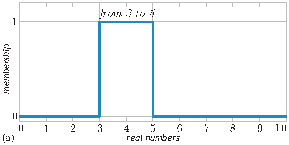
\includegraphics{fig_fuzzySet_a}
%		\caption{sub A}\label{labA}
%	\end{subfigure}
%	\hfill
%	\begin{subfigure}[b]{.5\figurewidth-3.5pt}
%		\noindent\hrulefill\par
%		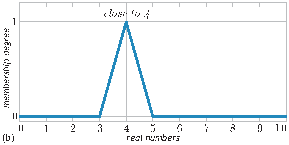
\includegraphics{fig_fuzzySet_b}
%		\caption{sub B}\label{labB}
%	\end{subfigure}
%	\caption{Membership functions of a crisp set of real numbers `from 3 to 5' \subref{labA} and a fuzzy set of real numbers `close to 4' \subref{labB}.}
%	\label{fig:fuzzy:set0}
%\end{figure}

\frontmatter
 	\maketitle
	\makeapprovedby
	\makepreviouspublication
 	% !TeX root = ./thesis.tex










%==============================
\cleardoublepage
\thispagestyle{empty}

\vspace*{55pt}

\begin{centering}

{\textsc{in memoriam}
 \par}

\vspace{.5cm}

{Damjan Oseli
 \par}

{1975--2004
 \par}

\end{centering}

\vfill






%==============================
\cleardoublepage
\thispagestyle{empty}

\vspace*{55pt}

\begin{centering}

{\setbox0=\hbox{\emph{``Things never turn out the way you think they will.''}}
 \begin{minipage}{\wd0}
 \emph{``Things never turn out the way you think they will.''}\\
 \null \hfill  --- Michael Crichton, \emph{Prey}, 2002.
 \end{minipage}
 \par}

\vspace{.5cm}

{\setbox0=\hbox{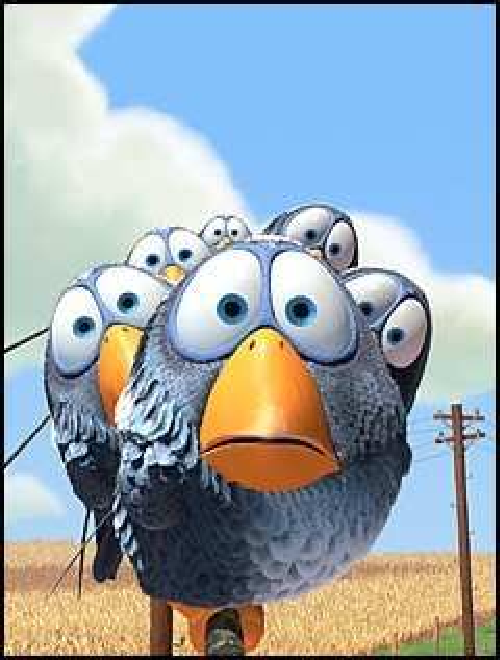
\includegraphics{pixar_forTheBirds}}
 \begin{minipage}{\wd0}
 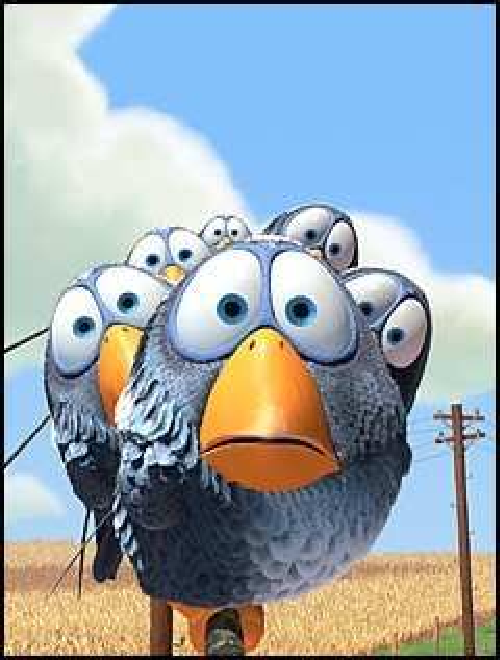
\includegraphics{pixar_forTheBirds}\\
 \null \hfill  --- Pixar, \emph{For the Birds}, 2000.
 \end{minipage}
 \par}

\end{centering}

\vfill
\cleardoublepage

 	% !TeX root = ./thesis.tex

% write thesis abstracts
% use \begin{abstract}\end{abstract} for abstract in english
% use \begin{povzetek}\end{povzetek} for abstract in slovene
% note
% with english as primary language the order is povzetek, abstract
% with slovene as primary language the order is abstract, povzetek


%==============================
\begin{povzetek}

%-----
\lipsum[2-4]

\end{povzetek}


%==============================
\begin{abstract}

%-----
\lipsum[2-4]

\end{abstract}

 	% !TeX root = ./thesis.tex

% Do thank those that have helped you








%==============================
\begin{acknowledgements}

Along my epic journey as a PhD student I was lucky enough to have met and shared parts of this pilgrimage with a number of interesting characters. Not to leave anyone out or have the acknowledgements take the major part of this book, I will, from now on, write as if we all contributed to this work (in fact we did, one way or another).

\end{acknowledgements}

\vfill

\begin{center}
	\textsc{This thesis was partially funded by the European Social Fund.}
	
	\vspace{.2cm}
	
	\textsc{Credits for the stuning photo on the cover go to Ed Ralph.}
\end{center}
 	\tableofcontents 

\mainmatter
 	% !TeX root = ./thesis.tex










%==============================
\chapter{Introduction}
\label{ch:introduction}


%-----
\section{Motivation}
With the increase of the processing and presentational capabilities of personal computers, the field of computer modelling and simulation has been gaining research interest even in the areas that a decade ago did not believe that modelling and simulation were suitable for them. One such area is the modelling of the dynamics of organized groups of moving animals. Some of the typical examples of such groups are pedestrians \cite{brogan:1998,helbing:1995}, bird flocks and fish schools \cite{aoki:1982,heppner:1990,lebar_bajec:2002,lebar_bajec:2003a,lebar_bajec:2003b,lebar_bajec:2005a,okubo:1986,reynolds:1987,terzopoulos:1994,tu:1994,tu:1999,zaera:1996}, ant colonies \cite{bonabeau:1999,resnick:1997}, \etc\ For the majority of these groups their dynamics is not based on a centralized source of decision processing, but on a distributed one. Each individual member of the group thus processes its own decision, depending on the perceived state of the universe and the tendencies that originate from the drives guiding it.

If I focus on bird flocks: the first and most influential models were developed by Reynolds \cite{reynolds:1987} and Heppner and Grenander \cite{heppner:1990}. In both cases the drives are implemented through mathematical equations (geometrical calculations, differential equations, \etc), which the authors obtained by means of trial-and-error experimentation. According to Reynolds \cite{reynolds:1987,reynolds:1999}, these drives are:

\begin{itemize}
  \item \emph{separation}: each member of the flock tries to maintain a certain separation distance from its flockmates (nearby flock members),

  \item \emph{alignment}: each member of the flock tries to match its flight speed and flight direction with that of its flockmates,

  \item \emph{cohesion}: each member of the flock tries to fly toward the centre of its flockmates.
\end{itemize}

According to Heppner and Grenander \cite{heppner:1990}, the drives are:

\begin{itemize}
  \item \emph{homing}: each member of the flock tries to stay in the roosting area,

  \item \emph{velocity regulation}: each member of the flock tries to fly with a certain predefined flight speed---it tries to return to that speed if perturbed,

  \item \emph{interaction}: if two flockmates are too close to one another, they try to move apart; if they are too distant, they do not influence each other; otherwise they try to move closer together.
\end{itemize}

However, in addition to these three drives, Heppner and Grenander modelled also the \emph{random impact}, which was intended to simulate the random distractions that are present in a natural environment (wind gusts, distractions from moving objects on the ground, \etc). They implemented it as a Poisson stochastic process and admitted that without its inclusion they were unable to produce flock-like behaviour.

Upon the analysis of the relevant bibliography it has been determined that the existing models have some weaknesses, which can be briefly summarized as follows:

\begin{itemize}
  \item \emph{syntactical confusion}: most of the authors do not present formal definitions of the models; in the majority of cases the models are only described, which is usually not a good enough basis for an actual implementation; the latter requires a formal specification in the form of an automaton or algorithm;

  \item \emph{lack of evaluation metrics}: regardless of the numerous models, neither an analytical comparison between the obtained results nor their evaluation have been performed; in this sense the models have never been truth-tested;

  \item \emph{usability}: most of the models are based on complex mathematical formalisms (differential equations, random processes, computation of the centre of mass, \etc); in this sense the models are difficult to understand and/or use by the audience they were designed for (biologists, ethologists, behaviourists, etc.).
\end{itemize}

Fuzzy modelling has gained momentum with the increase of processing capabilities. It is based on fuzzy logic, which emerged as an outgrowth of fuzzy set theory. The latter was first introduced in 1965 by Lotfi A. Zadeh \cite{zadeh:1965}. Fuzzy set theory is a generalization of conventional (or crisp) set theory by the introduction of the concept of partial membership. The main difference between the two is thus in the interpretation of membership. In conventional set theory, an object can be either a member of the observed set or not a member of the observed set; in fuzzy set theory, however, it can also be a partial member of the observed set. Therefore if the object's membership to the observed set is computed by means of a membership function, then in the case of a crisp set this function maps to the set $\left\{0,1\right\}$, whereas in the case of a fuzzy set it maps to the entire unit interval $\left[0,1\right]$.

The basics of modelling using uncertain knowledge and preconditions were set by Witold Pedrycz \cite{pedrycz:1993}. In the current literature numerous examples of fuzzy modelling can be found (modelling of fire spread prediction \cite{mraz:1999,vakalis:2004a,vakalis:2004b}, modelling of snow avalanches \cite{barpi:2004}, modelling of the control of kitchen appliances \cite{mraz:2001}, \etc). However, only some of them model massive dynamic processes. Furthermore in the extensive literature I did not find any attempt at fuzzy modelling of bird flocking.


%----
\section{Scientific Contributions}
In the light of the preceding discussion about the existing models' weaknesses, the following scientific contributions are presented in this dissertation:

\begin{itemize}
  \item \emph{design and formal definition of an extended Moore automaton (animat)}:
  with respect to the current syntactical confusion I design and present a formal definition of an extended Moore automaton \cite{kohavi:1978}, which allows a uniform approach to modelling the dynamics of organized groups of moving entities; the ideas behind the above mentioned formal definition correspond with the term animat, which was introduced, without a formal definition, by Wilson \cite{wilson:1985}; in spite of that, in the last decade the term has become the synonym for a class of computer simulated animals or robots;

  \item \emph{design and formal definition of a fuzzy extended Moore automaton (fuzzy animat)}:
  afterwards I upgrade the extended Moore automaton with the introduction of fuzziness \cite{zadeh:1965}; the latter allows the construction and implementation of the automaton by using ambiguous (uncertain, vague, \etc) knowledge and data; one of the main advantages of fuzzy logic is its ability to permit a direct linguistic description (programming) of an arbitrary decision system;

  \item \emph{application of the fuzzy animat to the problem of the simulation of bird flocking}:
  to present its usability I employ the fuzzy animat to model a member of a bird flock; the model is limited to a two-dimensional space without obstacles; these two preconditions originate from comparable models of other authors;

  \item \emph{design and formal definition of a set of metrics used for comparing the simulation results from different computer models of bird flocking}:
  the authors of the related models base the analysis of their simulation results mostly on visual grounds; the approach is subjective and is, as such, useless for an analytical comparison of different models; with this in mind I design and formally define a set of metrics that allow the comparison of the simulation results, and if the required data be available, perhaps also a comparison to the dynamics of a natural flock;

  \item \emph{comparison of the simulation results obtained by using different computer models of bird flocking}:
  I then use the introduced metrics to compare the simulation results obtained by using the newly introduced model with those obtained by using Reynolds's model \cite{reynolds:1987,reynolds:1999}; the latter represents the main reference for the majority of the existing models;

  \item \emph{analysis of simulation results from different computer models of bird flocking}:
  I analyse the differences in the simulation results of the compared models.
\end{itemize}


%----
\section{Methodology}
In the quest to achieve the discussed scientific contributions, the following methodologies have been employed:

\begin{itemize}
\item review and analysis of the bibliography related to modelling massive dynamic processes; in doing so, I have learnt about the most important related models;
\item application of the acquired knowledge to the design of an extended Moore automaton (animat);
\item application of the knowledge about fuzzy logic to the design of a fuzzy extended Moore automaton (fuzzy animat);
\item development of a computer application (simulator) for the simulation of bird flocking;
\item experimental work with the simulator and analysis of the simulation results;
\item comparison of the results obtained with the simulation and those obtained by using the computer models of other authors;
\item monitoring and review of all of the new activities in the related fields and active participation in the form of journal articles and conference contributions.
\end{itemize}


%----
\section{Dissertation Overview}
The main question to be addressed by this dissertation is, ``How to use fuzzy logic for modelling bird flocking?'' I feel that flock-like behaviour could be much more easily described by using simple linguistic descriptions (\eg\ collections of if-then rules) than by using mathematical equations. Indeed, the existing knowledge about the behaviour of flocks is usually available in the form of the observer's linguistic descriptions and explanations of the perceived behaviour.\footnote{``\emph{It seems likely that if a bird, say, to the left and in front of another bird turned suddenly in front of the trailing bird, the trailing bird would have time to react, and turn in the same direction, avoiding collision.}'' From personal correspondence with Frank H. Heppner.} The existing models were thus arrived at by approximating such linguistic descriptions using mathematical equations. Moreover, considerable amounts of advanced mathematical skills were required for this transition. Fuzzy logic \cite{zadeh:1965} is a very popular, successful and widespread approach for modelling processes, for example fire spread prediction \cite{mraz:1999,vakalis:2004a,vakalis:2004b}, which are too complex for classical mathematical methods. I feel that by using it to describe the simulated animal's behaviour the transition from the linguistic description to the actual behaviour could be made much shorter and much more understandable. In this way researchers involved with the study of the dynamics of organized groups of moving animals would gain a tool that enabled them to construct the subjects of their interest---the digital animals---and study their behaviour through simulations.

This dissertation presents the \emph{fuzzy animat construction framework} and through the study case of bird flocking also its usage. In \chaptername~\ref{ch:birdFlocks} the bird flocking literature is reviewed and the two most influential models are presented. \chaptername~\ref{ch:animat} presents a formal definition of an extended Moore automaton that can be used as a uniform approach to modelling the dynamics of organized groups of moving animals. \chaptername~\ref{ch:fuzzyModelling} presents a brief overview of fuzzy logic and fuzzy modelling. In \chaptername~\ref{ch:fuzzyAnimat} fuzzy logic is used to introduce fuzziness into the earlier formalized extended Moore automaton, which is then used to construct a fuzzy digital bird. \chaptername~\ref{ch:analysis} is dedicated to the analysis of the dynamics of organized groups of moving fuzzy digital birds and \chaptername~\ref{ch:conclusion} concludes by reviewing the achieved scientific contributions and presenting the future research directions.

I assume that the reader is familiar with the fundamentals of the theory of conventional (or crisp) sets and conventional (crisp or two-valued) logic. Furthermore, it is assumed that the reader is familiar with Euclidean vector spaces and corresponding vector operations. Throughout the dissertation I use the following notation:

\begin{itemize}
  \item $\N=\left\{1,2,3,\ldots\right\}$ the set of all positive natural numbers,
  \item $\N_n=\left\{1,2,3,\ldots,n\right\}$ the set of all positive natural numbers lower or equal $n$,
  \item $\R$ the set of all real numbers,
  \item $\R^+$ the set of all non-negative real numbers,
  \item $\E$ an Euclidean vector space such as $\R^2$, $\R^3$,
  \item $\set{A},\ldots,\set{Z}$ conventional (or crisp) sets,
  \item $\fset{A},\ldots,\fset{Z}$ fuzzy sets,
  \item $\vect{a},\ldots,\vect{z}$ vectors from vector space $\E$,
  \item $\langle x_1,x_2,\ldots,x_n \rangle$ ordered $n$-tuple of elements $x_1$, $x_2$, \ldots, $x_n$.
\end{itemize}

\noindent In addition
\begin{itemize}
  \item $\mathrm{iff}$ is shorthand expression for ``if and only if'',
  \item $\exists$ is shorthand expression for ``exists'',
  \item $\forall$ is shorthand expression for ``for all'',
  \item $\left|\set{A}\right|$ is shorthand for the size of set $\set{A}$,
  \item $\mu_\set{A}$ is shorthand for the membership function of crisp set $\set{A}$,
  \item $\powset{\set{A}}$ is shorthand for the family of all crisp sets that can be defined on universal set $\set{A}$,
  \item $\mu_\fset{A}$ is shorthand for the membership function of fuzzy set $\fset{A}$,
  \item $\fpowset{\set{A}}$ is shorthand for the family of all fuzzy sets that can be defined on universal set $\set{A}$,
  \item $\left\|\vect{a}\right\|$ is shorthand for the size (norm) of vector $\vect{a}$,
  \item $\vect{a}^0$ is shorthand for the normalized vector $\vect{a}$ (\ie\ a vector in the same direction as $\vect{a}$ but with size $1$),
  \item $\lfloor\vect{a}\rceil^a$ is shorthand for the truncated vector $\vect{a}$ (\ie\ a vector in the same direction as $\vect{a}$ but with size lower or equal $a$).
\end{itemize}

 	% !TeX root = ./thesis.tex










%==============================
\chapter{Bird Flocks}
\label{ch:birdFlocks}


%-----
\section{Flock Formations}
Of all coordinated groups of moving vertebrates, birds are at the same time the easiest to observe and perhaps the most difficult to study \cite{heppner:1997}. This is primarily because most of the animal congregation research is highly dependent on collecting \cite{heppner:1997,jaffe:1997} large sets of four-dimensional data (\ie\ three in space and one in time). In fact, as a contrast to birds, most mammals move in a two-dimensional plane, which simplifies obtaining real-world data, and fish can be brought into a laboratory and enclosed in an aquarium for study. Probably because of the easier and more fruitful tracking of confined objects \cite{heppner:1997,parrish:1997a}, fish schools have been a frequent research theme \cite{aoki:1982,dill:1997,mcfarland:1997,partridge:1982,shaw:1962,terzopoulos:1994,tu:1994,tu:1999,ward:2001,zaera:1996}. 

On the other hand, scientists involved in bird congregations research are challenged by the highly difficult and almost luck-dependent data collection \cite{heppner:1997}. Just the fact that a single bird in an organized flock can move through six degrees of freedom at velocities up to 150 km/h makes collecting real-world data very difficult. Flocks fly in a three-dimensional space that cannot be easily contained and their flight paths cannot be predicted. Even by knowing the locations where there is a reasonable probability of flock appearance one cannot predict its flight path. Furthermore the three-dimensional acquisition and analysis techniques generally demand either fixed camera or detector positions. The free-flying flocks must thus be either induced to fly in the field of the cameras or the cameras must be placed in locations where there is reasonable probability that adventitious flocks will move through their field. The difficulty of data acquisition is evident even from the existing literature \cite{gould:1974,heppner:1997,jaffe:1997,moyle:1998}. According to Heppner \cite{heppner:1997}, this may be one of the reasons why there is a current of imaginative speculation, and lively controversy in literature on bird congregation structure and internal dynamics, but little data. However, regardless of the difficulty of data acquisition, some basic understanding of bird flocks is already available. 

Birds can fly in disorganized groups, such as gulls orbiting over a landfill, or organized groups, such as the vees of waterfowl. To the evolutionist, behaviourist, or ecologist, any group is of interest, but nevertheless organized groups raise most questions. In his pioneering work from 1974 Heppner \cite{heppner:1974a} presented the first definitions of the two groups. 

\begin{definition}
	\label{def:aggregation}
	A disorganized group of birds or \emph{flight aggregation} is a group of flying birds lacking coordination in turning, spacing, velocity, flight direction of individual birds and time of take-off or landing, assembled in a given area.
\end{definition}

\begin{definition}
	\label{def:flock}
	An organized group of birds or \emph{flight flock} is a group of flying birds, coordinated in one or more of the following parameters of flight: turning, spacing, velocity, and flight direction of individual birds, and time of take-off and landing.  
\end{definition}

In this study Heppner also presented a classification of flight flock formations and a discussion of the leading research directions.\footnote{In this dissertation I primarily consider groups of birds in flight and thus will be concerned neither with their take-off nor landing. For reasons of clarity the term flight in flight flock and flight aggregation will therefore be omitted.} According to his study, there are two major classes of flight formations: \emph{line formations} and \emph{cluster formations}. Their characteristics had and still have a substantial influence on the leading research directions. Today \cite{heppner:1997,parrish:1997a}, as it was then \cite{heppner:1974a}, the examination of bird flocks is still led by two primary questions. The first, usually expressed while observing a skein of geese flying overhead, is ``\emph{Why do they fly in such a precise alignment?}'' The second comes to mind when we observe 5000 European Starlings, \emph{Sturnus vulgaris}, turning and wheeling over a roost. We ask ourselves ``\emph{How do they achieve such coordination and polarity?}'' The question `why' is thus usually expressed in reference to relatively large birds, like waterfowl, flying in line formations, whereas the question `how' is in reference to relatively large flocks of small birds, like sandpipers, flying in cluster formations. 

%--
\subsection{Line Formations}
Line formations (\fig~\ref{fig:lineFormations}) are groups of relatively large birds, such as waterfowl and pelicans, flying in a single line, or joined single lines. Typically they are approximately two-dimensional and show a rather high degree of regularity in spacing and alignment. In line formations birds fly in a single line, one behind the other (\emph{column}), one beside the other (\emph{front}) or staggered stepwise from the bird at the head of the formation (\emph{echelon}). In nature left and right echelons can be found and frequently a left echelon becomes a right echelon, and vice versa. However, the transition is not a swing from side to side, but rather a temporary breakup of the formation. In line formations birds also fly in joined single lines; left and right echelons joined at the tip of the formation (\emph{`J'} and \emph{`V'}) or at the tail of the formation (\emph{inverted `J'} and \emph{inverted `V'}). In the `V' and inverted `V' formation the left and right echelon are approximately the same size, whereas in the `J' and inverted `J' formation one is considerably larger.

\begin{figure}
	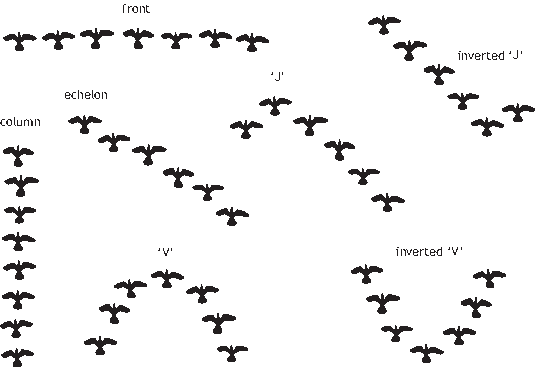
\includegraphics{fig_lineFormations}
	\caption{Line formations: column, front, echelon, `J', `V', inverted `J', and inverted `V' \cite{heppner:1974a}.}
	\label{fig:lineFormations}
\end{figure}

%--
\subsection{Cluster Formations}
Cluster formations (\fig~\ref{fig:clusterFormations}) are relatively large flocks of small birds, like sandpipers, characterized by development in the third dimension, and rapid, apparently synchronous turns. In cluster formations birds are typically distributed over a three-dimensional space of an irregular spheroidal shape that is, when observed perpendicularly to the plane of flight: as wide as it is long (\emph{globular cluster}), wider than it is longer (\emph{front cluster}), or longer than it is wider (\emph{extended cluster}). Birds flying in globular clusters generally fly in apparent close order and can be seen making very rapid turns. Similarly, front clusters tend to have very precise spacing and turning. The front cluster is often seen in pigeons. However, birds flying in extended clusters tend to be rather disorganized, with frequent breakoffs and shifts of position. This formation may simply be a disorganized group of birds that happen to be flying independently toward a common destination (\ie\ an aggregation) \cite{heppner:1974a}.

\begin{figure}
	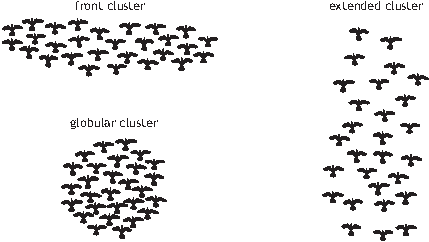
\includegraphics{fig_clusterFormations}
	\caption{Cluster formations: front cluster, globular cluster, and extended cluster \cite{heppner:1974a}.}
	\label{fig:clusterFormations}
\end{figure}


%-----
\section{Simulating Bird Flocks}
While observing line formations, one is impressed by the precision with which relatively small numbers of large birds maintain themselves in accurate spatial alignment and angular orientation with their flockmates. On the other hand, while observing cluster formations, the attention is drawn to the coordination that enables large numbers of small birds, flying in close order, to wheel and turn without suffering mid-air collisions. In the first case the primary interest is the functional significance of formation flight \cite{heppner:1997,speakman:1998}. In the second the attention is given to the synchrony, or apparent synchrony, in the turning movements and the necessity or presence of a leader guiding these manoeuvres.

In the mid 1980s different papers appeared, suggesting that coordination in cluster flocks might be achieved by the application of the mathematics of nonlinear dynamics \cite{okubo:1986} and that flocking might be an emergent property arising from individuals following simple rules of movement \cite{heppner:1987}. At the same time, but working in another field of study, namely computer graphics, Reynolds \cite{reynolds:1987} published a ground-breaking seminal paper that first presented a computer model of bird flocking. His primary objective was a believable animation of a bird flock. In his study a collection of individuals whose behaviour is governed by three simple rules based on geometrical calculations, demonstrates flocking behaviour that is typical for flying birds. Without knowing about Reynolds's work, ornithologist Frank Heppner joined forces with mathematician Ulf Grenander and published the second computer model of bird flocking \cite{heppner:1990}. In their model the flock was a self-organizing collection of individuals, whose behaviour was based on stochastic nonlinear differential equations. Nevertheless, both models base their assumptions on common grounds and model the behaviour of individuals on the, at times contradictory, clues of attraction and repulsion. The mutual coexistence and importance for the congregation's structure of these two clues was already suggested by Okubo \cite{okubo:1980}.

After 1990 papers regarding computer models of bird flocking subsided. The rare exceptions were the studies of the evolution of flocking behaviour \cite{reynolds:1993a,reynolds:1993b,reynolds:1994,spector:2002,spector:2003} and Heppner's unpublished study of flock take-off and landing \cite{heppner:1997}. In the last few years the field has been slowly regaining scientific interest. Recent research, however, builds on the two original models. Tanner, Jadbabaie, and Pappas \cite{tanner:2003a,tanner:2003b} for example concentrate on the stability analysis of an organized flock that is based on Reynolds's model. Couzin \etal\ \cite{couzin:2005}, on the other hand, employ Reynolds's model to examine leadership and decision making in animal groups on the move. Their approach adds a preferred flight direction only to a proportion of the modelled digital birds. Their study reveals that the larger the group the smaller the proportion of informed individuals needed to guide the group, and that only a small proportion is required to achieve great accuracy. A rare example of a different, and also the most recent, approach is that of Wiltschko and Nehmzow \cite{wiltschko:2005}, but its primary concern is not flocking but rather the navigation process employed by pigeons. 

The primary reasons for the loss of research interest may lie hidden in the mathematical nature of these simulations as well as in the amount of work that is required to master the effects that parameter changes have on the displayed behaviour. Even Heppner and Grenander \cite{heppner:1990} admit that the interesting patterns were discovered serendipitously and that considerable trial-and-error experimentation was needed before flock-like behaviour was produced.

In addition, one can hardly imagine that flocking birds flying at speeds up to 150\,km/h \cite{heppner:1997} have the time or the ability to perform sophisticated or time-intensive mathematical calculations. Even Parrish \etal\ \cite{parrish:1997a} state that there must be simple traffic rules for species' engaging in collective movement. To continue, considering our perception of the surrounding environment, it is difficult to imagine that birds are able to perceive precise (\ie\ crisp) information (\eg\ distance). However, all of the existing mathematical models assume such capabilities.

Furthermore, the mathematical nature of the existing models means that a substantial mathematical understanding was required for their construction as is required for their thorough understanding. In my opinion this represents a major drawback for their usability. The mathematical nature, if truth be told, makes the models difficult to understand by the audience they were designed for. The latter is predominantly composed of ethologists, not mathematicians. Even if one makes the models as black-box modules and allows only changing the values of parameters, this would not suffice for truth-testing. Truth-testing any sort of simulation that purports to represent natural behaviour is extremely difficult, and has not often been done, especially in behaviour. Models are usually too crude, or have too many special conditions to be readily tested with real-world data. This is probably why ethologists have difficulties in using the models for testing the existing hypotheses or forming new ones.

%--
\subsection{Computer Model by Craig W. Reynolds}
\label{subsec:birdFlocks:cwr}
Traditionally an animator who wanted to animate a bird flock would carefully set up numerous key frames that defined the motion paths of every single flock member. When animating a line flock, especially if it is a very small one, such an approach is somehow possible. Difficulties arise when large cluster flocks are being animated. In this case animating each and every flock member becomes painstaking and tedious, and is, disregarding the difficulty of corrections, without inter-bird collisions almost impossible to do. 

As already mentioned, Craig W. Reynolds, in his pioneering work from 1987, presented the first computer model of bird flocking \cite{reynolds:1987}. When reflecting on how to animate a bird flock he treated the latter as any group of entities that exhibit the general class of aligned, noncolliding, aggregate motion. This means that with the term flock Reynolds refers also to schools, herds, \etc\ However, when speaking about bird flocks it can be seen that his notion is more strict than definition~\ref{def:flock}. In fact, he assumes an organized flock to be coordinated in all of the flight parameters as well as that there are no collisions. However, the requirements of definition~\ref{def:flock} are met also when coordination is only in some of the parameters of flight and the definition does not make note of the absence of collisions. The latter on one hand seems plausible, however, on the other hand, especially in large cluster flocks, because of their size, the relatively small inter-bird spacing and fast manoeuvres, seems almost impossible.

In the mid 1980s the decentralization ideology \cite{resnick:1997} was becoming ever more influential. This was also the time when the research field of \emph{artificial life} \cite{adami:1998,emmenche:1994,langton:1989} was emerging. Both, together with Reynolds's prior work \cite{reynolds:1978,reynolds:1982}, led him toward the idea that a flock of birds, as perceived by one of its members, is something completely different than as perceived by an outside observer. It is much like the difference between driving in traffic and standing on a roadside watching traffic whiz by. This represented an important step forward. He did not look at the flock as a whole any more or searched for a single rule that describes it---known as \emph{top-down approach}. On the contrary, he imagined what it would be like to be a member of the flock and searched for the rules to follow in order to stay in the flock---known as the \emph{bottom-up approach}. This approach is characteristic for modelling artificial life \cite{adami:1998,emmenche:1994,gardner:1970,langton:1984,langton:1989,rucker:1993,terzopoulos:1994,terzopoulos:1999,tu:1999,ward:2001}. I am talking about modelling by constructing a large number of primary entities, whose local interactions base on simple rules, and observing the emergent global behaviour, behaviour not previously programmed according to specific rules \cite{emmenche:1994}. Later, in computer graphics, Reynolds's approach, when one actually seeks to model the behaviour of an object and not its shape or physical properties,  became known as \emph{behavioural animation} \cite{reynolds:1987}.

Reynolds \cite{reynolds:1987} came to the conclusion that as a member of a flock he would have to successfully coordinate three different drives. He found out that, in order to fly without collisions, he would have to make sure that he was not too close to any of his flockmates. In other words, he would try to maintain a certain separation distance. Furthermore, he would have to try to fly with the same flight speed and in the same flight direction as his flockmates. This also means that it would be highly unlikely that he collided with them in the near future. And finally if he noticed that all of the flockmates were on one of his sides he would wish to drift towards them. Written in the form of simple rules these drives are \cite{reynolds:1987,reynolds:1999,reynolds:2000}:

\begin{itemize}
	\item {\emph{separation}}: avoid collisions with nearby flockmates,
	\item {\emph{alignment}}: attempt to match flight speed and flight direction with nearby flockmates,
	\item {\emph{cohesion}}: attempt to stay close to nearby flockmates.
\end{itemize}

The cohesion and separation drives, when viewed in unison, represent the so-called \emph{attraction-repulsion} scheme \cite{okubo:1980}. The alignment drive, on the other hand, is used to produce \emph{polarization}, which is another important feature of animal groups of uniform density \cite{parrish:1997a}. 

Reynolds translated the three drives to a set of geometrical equations, where he interpreted the expression `nearby flockmates' as the bird's immediate surroundings (see subsection~\ref{subsec:birdFlocks:cwr}). Actually, he found out that a bird does not require full knowledge about the positions, flight speed and flight direction of every bird in the flock, but only a small subset. The expression `nearby flockmates' thus addresses the bird's awareness of another bird and Reynolds based its computation on the distance and direction of the offset vector between them. His digital bird\footnote{Actually Reynolds refers to the digital (simulated) bird-like, ``bird-oid'' objects, generically as \emph{boids} even when they represent other sorts of creatures such as schooling fish \cite{reynolds:1987}.} thus actually has a localized perception of the world with a certain distance and field of view and can be visualized as a perception volume shaped like a sphere with a cone removed from the back. It is important to note that, when the digital birds are in a flock, the individual perception volumes overlap and each individual bird will probably end up in a number of perception volumes.

With a limited perception volume, Reynolds makes a very good point stating that a bird's perception of the world is severely limited by occlusion (\ie\ nearby birds hide those far away), but inside the perception volume he does not take this into account. Furthermore, even though he limits the digital bird's awareness of the world, the perceived information is accurate, meaning that the digital bird has full and precise knowledge about the position, flight speed and flight direction of its flockmates. In my opinion this approach is still defective. It is true that Reynolds does not try to model visual perception but tries to make available approximately the same information that is available to a bird as the end result of perceptual and cognitive processes. However, all of the obtained information is still based on visually perceptible information. A bird's visual perception is not limited only by occlusion, but also by the fact that the ability to sense distance, apart from being affected by the degree of binocular overlap, decreases with distance itself. Moreover, in his latest implementation of the model,\footnote{OpenSteer v0.8, \href{http://opensteer.sourceforge.net/}{http://opensteer.sourceforge.net/}.} Reynolds uses three distinct perception volumes, one per drive. According to my experiments (see \chaptername~\ref{ch:analysis}) this introduces unwanted `unnatural' behaviour.

Furthermore, Reynolds models the cohesion drive as the digital bird's tendency to fly toward the centre of mass of the nearby flockmates. I find this somewhat questionable. The centre of mass is a mathematical construct and it is difficult to believe that a real bird has knowledge of such constructs or uses them to compute its action. It is true that it was Pliny \cite{heppner:1997} who noted that ``it is a peculiarity of the starling kind that they fly in flocks and wheel round in a sort of circular ball, all making towards the centre of the flock''. However, in my opinion, real birds might not have any idea about the centre of the flock and their making towards it might be just an emergent property by itself.

In Reynolds's approach an individual digital bird thus, based on the precise information about the position, flight speed and flight direction of its flockmates, using geometrical equations, computes the three desired changes of flight direction and flight speed, each satisfying one drive. As Reynolds models the digital bird as a point mass (simple) vehicle \cite{reynolds:1987,reynolds:1999}, he represents the desired change in flight direction and flight speed as the physical force that would induce it. The digital bird thus computes the actual change in flight direction and flight speed by computing a weighted sum of the resulting three physical forces (see subsection~\ref{subsec:animat:cwr} for more detail).
 
%--
\subsection{Computer Model by Frank H. Heppner and Ulf Grenander}
\label{subsec:birdFlocks:fhh}
As a contrast to animators who try to produce a flock animation that visually resembles a natural flock in a way that could take in a theatre spectator, flocks interest ornithologists from a completely different point of view. The synchrony, or apparent synchrony, in the turning movements of cluster flocks has drawn much attention from ornithologists. The key research directions were, and still are, guided mostly by the question how flocks coordinate their movement and decide when to wheel or turn. With respect to this in most investigations the leading role was played by the search for evidence that would answer the question of existence or necessity of a flock leader. Indeed, many researchers assumed a leader's existence and presumed it directed the movement of the whole flock \cite{heppner:1990}. This approach was also taken by Heppner and Hafner \cite{heppner:1974b}, but they proceeded to demonstrate the formidable obstacles to visual or acoustic communication between such a putative leader and its followers. Nevertheless, efforts to identify the flock's leader have been so far unsuccessful, even when using methods that permit an analysis of the position of individually identified birds in a free-flying pigeon flock \cite{pomeroy:1992}. In the meantime reports appeared \cite{davis:1980} which suggested that the coordinated turning might be an emergent phenomenon; the result of individual birds `voting' with their bodies on the flight path the flock should take. According to this theory the flock turns in the direction expressed by the initiators only when a `critical mass' is reached. Recently, a similar approach has been used by Couzin \etal\ \cite{couzin:2005} to examine leadership and decision making in animal groups on the move.

Similar to Reynolds, ornithologist Frank H. Heppner started pondering the idea that flocks might be an emergent phenomenon; the result of a group of individuals following simple rules. This idea was, again as in Reynolds's case, initially inspired by artificial life research; by Conway's `Game of Life' \cite{gardner:1970}, to be more precise. Moreover, also by the emerging suggestions that coordination in cluster flocks could be achieved by the application of nonlinear dynamics \cite{okubo:1986}. As ornithologists in most cases are not mathematicians, Heppner joined forces with applied mathematician Ulf Grenander, to translate his ideas into mathematical equations. The result of their work was the second computer model of bird flocking \cite{heppner:1990} given through a stochastic differential driven by a Poisson process. As in Reynolds's case, the model developed by Heppner and Grenander also suggested that birds coordinate through three, but different drives. They assumed that the coordination in flocks emerges because birds try to accomplish the following drives:

\begin{itemize}
	\item \emph{homing}: each member of the flock tries to stay in the roosting area,

	\item \emph{velocity regulation}: each member of the flock tries to fly with a certain predefined flight speed---it tries to return to that speed if perturbed,
	
	\item \emph{interaction}: if two flockmates are too close to one another, they try to move apart; if they are too distant, they do not influence each other; otherwise they try to move closer together. 
\end{itemize}

As already said, Grenander translated these drives into mathematical equations that depended on the current position of the digital bird (homing), its flight speed (velocity regulation) or its distance from other digital birds (interaction). But their digital bird has complete and precise information about the locations of other digital birds. With this Heppner and Grenander make an unrealistic assumption because, as already discussed, real birds have limited and inaccurate perceptive capabilities.

As a contrast to Reynolds, who modelled the principles of attraction and repulsion in the form of two distinct drives, Heppner and Grenander combined them into one drive (interaction). Combined or not, the two drives seem reasonable and `natural', after all, their mutual coexistence and importance for the congregation's structure has already been suggested by Okubo \cite{okubo:1980}. On the other hand, the velocity regulation drive used by Heppner and Grenander seems somewhat strange. They derived this drive from aerodynamic theory; with a given power output and configuration, an aircraft will maintain a constant speed, it will return to that speed if perturbed. A real bird would not have to make a decision about this. In my opinion, this results in a questionable effect. Take, for example, a digital bird that slowed down because it was too close to one of its flockmates. It will speed up. But not because it is trying to catch up with the flock, but because it is returning to the predefined preferred flight speed. In my opinion this behaviour resembles more to an aggregation of birds that happen to be flying together than to a flock of birds that are trying to fly together. Furthermore, it is hard to grasp that a bird has a predefined preferred flight speed. Even if it does, this cannot be constant in time. Even though birds (especially in line flocks) tend to fly in relatively straight lines and at very consistent speeds, they tend to change their flight speed regardless of the speed of the flock, which might, however, be primarily caused by fatigue or other distractions (\eg\ wind gusts). 

Another important feature of flocks is alignment. Heppner and Grenander \cite{heppner:1990} did not model it specifically, but they mention that in certain cases organized flocks maintaining straight direction of flight emerged. This might be caused by the perception model they used. Their digital bird has complete and accurate information about its surroundings, which means it has full and precise knowledge about the locations of all surrounding digital birds that are closer than a predefined distance. However, in their quest for realism, Heppner and Grenander, introduced also a special influence which was intended to simulate the effects of wind gusts and random local disturbances. They modelled it using a Poisson stochastic process and state that it was of crucial importance for achieving flock-like behaviour \cite{heppner:1990}.

 	% !TeX root = ./thesis.tex










%==============================
\chapter{The Animat}
\label{ch:animat}


%-----
\section{The Digital Universe}
The first attempts to model artificial life date all the way back to the 1940s. It was then when John von Neumann, while researching advanced computer structures, based on parallel processing, laid the foundations of a special structure denoted as a \emph{cellular automaton}. Indeed, most of the early artificial life research was based on the cellular automaton, Conway's `Game of Life' \cite{gardner:1970} and Langton's self-reproducing loop \cite{langton:1984} being the most renown examples \cite{adami:1998,emmenche:1994,rucker:1993}.

The cellular automaton is formally defined as a \emph{spatial array} of \emph{cells}, where each cell holds a \emph{digital state number} \cite{rucker:1993}. The cells' states are updated in \emph{parallel} at \emph{discrete time steps}. In addition, it is required that the method of updating is \emph{local} and \emph{homogeneous}. In most cases the cells' next states are computed based on their current state and the state of their immediate neighbourhood (\ie\ the states of the cells that are, with respect to their spatial arrangement, adjacent to the observed cell). But the fixed topology of the cellular automaton makes it difficult to apply to modelling the dynamics of organized groups of moving animals. However, according to Mraz \cite{mraz:2000}, the abstract structure that is the most suitable for modelling a cell in the cellular automaton is the Moore automaton \cite{kohavi:1978}.

\begin{definition}
\label{def:Moore}
  The Moore automaton is defined as a five-tuple $\langle\set{X},\set{Q},\set{Y},\delta,\lambda\rangle$, where $\set{X}$, $\set{Q}$ and $\set{Y}$ are non-empty sets representing the input alphabet, the internal states and the output alphabet respectively; $\delta$ is a mapping called the transition function and $\lambda$ is a mapping called the output function:
  \begin{eqnarray}
    & \delta: \set{X}\times \set{Q}\rightarrow \set{Q}, & \\
    & \lambda: \set{Q}\rightarrow \set{Y}. &
  \end{eqnarray}
  At any discrete time step $t \in \set{T}$, where $\set{T}$ is a non-empty set of discrete time steps, the automaton is in a state $q(t) \in \set{Q}$. The state determines its future input-output behaviour. If an input $x(t) \in \set{X}$ is applied, then, in the next discrete time step $t+1$, the automaton assumes a new state $q(t+1) = \delta(x(t),q(t))$ that depends both on the current state and the input. In addition, the automaton emits the output $\lambda(q(t+1)) \in \set{Y}$, which depends on the new state.
\end{definition}

Let me put aside the cellular automaton structure and concentrate on its cell (\ie\ the Moore automaton). In this chapter the Moore automaton shall be extended so that it can be used to represent an inanimate or animate object. The idea of using Moore automata to represent inanimate or animate objects is not new; after all, every artificial life model constructed by using a cellular automaton makes this notion. However, instead of the fixed topology as required by the cellular automaton, a collection of extended Moore automata is not required to be in a fixed spatial arrangement. In other words this means that it can be used to represent the \emph{digital universe} \cite{bentley:2002}. Furthermore, it also means that the objects constituting the digital universe update their states in parallel at discrete time steps and that the method of updating is local yet not necessarily homogeneous.


%-----
\section{The Digital Animal}
\label{sec:animat}
Regardless of the methods used when modelling a digital animal, the basic characteristics of real animals first need to be abstracted. Most people accept or infer that every animal exists in time and space, and is surrounded by inanimate and animate objects (\ie\ the universe). Most people also presume that animals have senses (\ie\ sight, hearing, smell, \etc) through which they have the ability to \emph{perceive} the current state of the universe. An animal is, through \emph{actions} (\eg\ movement), capable of influencing its internal state and the state of the universe. With respect to its current internal state (\eg\ hunger) only certain data from the universe (\eg\ locations of food sources in the vicinity) is important to the animal and its \emph{drive} is to optimize (\eg\ minimize) the rate of their occurrence. The animal selects \emph{actions} (\eg\ feeding) that satisfy its drives. In view of its current internal state and the most pressing drives the animal performs a sequence of muscular movements that will accomplish a combination of these actions (\emph{action selection}). A model that takes into account the above characteristics is commonly referred to as digital (simulated, artificial) animal or \emph{animat} \cite{cliff:1993,watts:1998,wilson:1985}.

Modelling perception, drives and action selection with a Moore automaton is far from being straightforward. To simplify this, the Moore automaton was extended  \cite{lebar_bajec:2002,lebar_bajec:2003a,lebar_bajec:2003b} and the transition function $\delta$ from definition~\ref{def:Moore} reformulated to a three-stage scheme that is presented in \fig~\ref{fig:animat}. As the ideas behind the extension correspond with Wilson's animat \cite{wilson:1985}, I adopted the name and denoted the extended Moore automaton as an animat.

\begin{figure}
  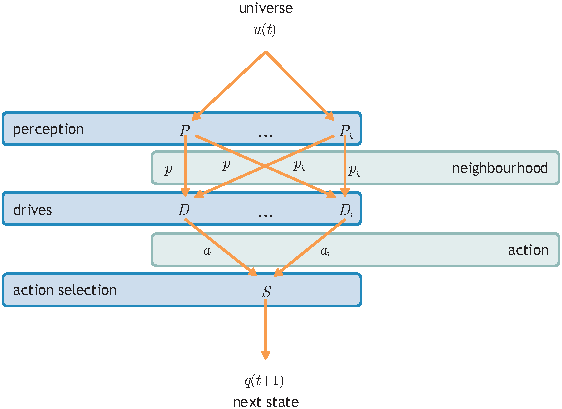
\includegraphics{fig_animat}
  \caption{The animat---the three-stage scheme of the reformulated transition function $\delta$.}
  \label{fig:animat}
\end{figure}

\begin{definition}
  \label{def:animat}
  An animat $\autom{A}=\langle\set{X},\set{Q},\set{Y},\delta,\lambda,P,D,S\rangle$ is an extended Moore automaton, where $P=\langle P_1,\ldots,P_k\rangle$, $D=\langle D_1,\ldots,D_l\rangle$, $S$ are a $k$-tuple of perception functions, an $l$-tuple of drive functions, an action selection function respectively and the transition function $\delta$ is defined as:
  \begin{eqnarray}
    & \delta(x,q) = S(\langle a_1,...,a_l\rangle,q), & \label{eq:animat:delta}\\
    & a_j = D_j(\langle p_1,...,p_k\rangle,q),\ j=1,\ldots,l, & \\
    & p_i = P_i(x,q),\ i=1,\ldots,k. & \label{eq:animat:Pi}
  \end{eqnarray}
\end{definition}

As already said, at the most basic level, the universe is a collection of inanimate and animate objects. I shall assume that it can be represented as a collection of animats (\ie\ extended Moore automata). This means that at a discrete time step $t \in \set{T}$ there are $n(t) \in \N$ animats. Nevertheless, without a loss of generality, it can be assumed that $n(t)=n,\ \forall t \in \set{T}$ and then the animats can be denoted as $\autom{A}_1,\ldots,\autom{A}_n$.

According to the discussion at the beginning of this section, animate and inanimate objects exist in time and space. Let $\E$ be an Euclidean vector space and $\set{S}_i$ represent the set of possible internal states of animal $i$. Then, when modelling organised groups of moving animals, the state of animat $\autom{A}_i$ at a discrete time step $t \in \set{T}$ is typically represented as $q_i(t)=\langle \vect{p}_i(t), \vect{v}_i(t), s_i(t) \rangle$, where $\vect{p}_i(t) \in \E$ denotes the position in space, $\vect{v}_i(t) \in \E$ the velocity and $s_i(t) \in \set{S}_i$ the internal state of the modelled animal.

Let $\set{Y}_i$ denote the output alphabet of animat $\autom{A}_i$ for all $i=1,\ldots,n$. It is a non-empty set representing data about animal $i$ that can be perceived by an outside observer. Therefore $\set{U}=\set{Y}_1 \times \cdots \times \set{Y}_n$ and the perceivable state of the universe at a discrete time step $t \in \set{T}$ is given by the $n$-tuple $u(t)=\langle y_1(t),\ldots,y_n(t)\rangle$, where $y_i(t)=\lambda_i(q_i(t))$ denotes the output of animat $\autom{A}_i$ at time step $t$ for all $i=1,\ldots,n$.

At any discrete time step all animats are applied the same input; the perceivable state of the universe. In other words, at a discrete time step $t \in \set{T}$, the input that is applied to all animats is $x(t)=u(t)$. Subsequently this means that all animats use the input alphabet $\set{X}=\set{U}=\set{Y}_1 \times \cdots \times \set{Y}_n$.

If I summarize: at a discrete time step an animat is applied the current perceivable state of the universe (\ie\ the data about all of the animats that can be perceived by an outside observer). Using the transition function (\ie\ taking into consideration perception, drives and action selection), the animat computes its next discrete time step state and then emits its new output. With this the perceivable state of the universe changes. In the following sections perception, drives and action selection are going to be discussed in more detail.

%--
\subsection{Perception}
As already said, the input of an animat is the current perceivable state of the universe. Let perception be the animal's process of \emph{interpreting} the perceivable data and \emph{selecting} just the relevant information from all of the sensory signals that exist in the universe (\eg\ detect the locations of food sources in the vicinity). From the viewpoint of human perception of the universe, it could be said that there exist multiple perception types (\ie\ sight, hearing, smell, \etc), where each of them selects only the relevant information according to a specific characteristic.

Let the current perceivable state of the universe be the $n$-tuple  $u=\langle y_1,\ldots,y_n\rangle$, where for all $i=1,\ldots,n$ $y_i \in \set{Y}_i$ is data about animat $\autom{A}_i$ that can be perceived by an outside observer. Let $q \in \set{Q}$ be the current state of the observed animat and let its input $x \in \set{X}$ be the current perceivable state of the universe, that is  $x=u=\langle y_1,\ldots,y_n \rangle$.

Let $\N_n$ denote the set of all positive natural numbers lower or equal to $n$ and for all $i=1,\ldots,n$ let the set $\set{I}^\textnormal{c}_i$ represent information about animat $\autom{A}_i$ that can be obtained from $y_i$ with respect to a certain characteristic $\mathrm{c}$.

Let the set $\set{N} \in \powset{\N_n}$ represent the set of indexes of members of $x$; in other words, animats that are according to characteristic $\mathrm{c}$ relevant to the observed animat. The ordered pair $p=\langle\set{N},o\rangle$, where $\set{N} \in \powset{\N_n}$ and $o \in \set{I}^\textnormal{c}_1 \times \cdots \times \set{I}^\textnormal{c}_n$ then represents the information regarding characteristic $\textnormal{c}$ that was obtained from the current perceivable state of the universe and is, with respect to this characteristic, relevant to the observed animat. For reasons of notational simplicity, let the set $\powset{\N_n} \times (\set{I}^\textnormal{c}_1 \times \cdots \times \set{I}^\textnormal{c}_n)$ be denoted simply as $\set{P}^\textnormal{c}$.

\begin{definition}
  \label{def:animat:Pi}
  Let $x \in \set{X}$ be the current perceivable state of the universe and $p \in \set{P}^\textnormal{c}$ be the information regarding characteristic $\mathrm{c}$ that was obtained from $x$ and is, according to this characteristic and the state $q \in \set{Q}$, relevant to the animat. Then a \emph{perception function} for characteristic $\mathrm{c}$ is a mapping $P: \set{X} \times \set{Q} \mapsto \set{P}^\textnormal{c}$.
\end{definition}

For reasons of simplicity I shall address the image of a perception function with the name \emph{neighbourhood}. If I sum up, a neighbourhood obtained by means of a perception function represents only the relevant characterized sensory signals (\eg\ locations of food sources in the vicinity). This means that the perception function allows taking into account that different animals employ different strategies for sampling sensory data \cite{cliff:1993}.

%--
\subsection{Drives}
The animal's drives are in strong correlation of its internal state and the perceived information about the state of the universe. In other words: based on the information obtained from the perceivable state of the universe (\eg\ locations of food sources in the vicinity) and its current internal state (\eg\ hunger) the animal will select actions (\eg\ feeding) that satisfy a specific \emph{drive} (\eg\ minimize hunger).

Let the observed animat have $k \in \N$ perception functions denoted as $P_1,\ldots,P_k$. This means that the set $\set{P}=\set{P}^{\mathrm{c}_1} \times \cdots \times \set{P}^{\mathrm{c}_k}$ represents information obtainable from the perceivable state of the universe. Let me for all $i=1,\ldots,k$ use $p_i \in  \set{P}^{\mathrm{c}_i}$ to denote the neighbourhood that was obtained using perception function $P_i$. Then $\langle p_1,\ldots,p_k\rangle \in \set{P}$ represents the perceived information about the current state of the universe that was, with respect to the current state of the animat, obtained from the current perceivable state of the universe.

\begin{definition}
  \label{def:animat:Dj}
  Let $\set{A}$ denote the set of possible actions of the animat and let $a \in \set{A}$ be the action that, with respect to the perceived information about the current state of the universe $\langle p_1,\ldots,p_k\rangle \in \set{P}$ and the current state of the animat $q \in \set{Q}$, satisfies a specific drive. Then a \emph{drive function} is a mapping $D: \set{P} \times \set{Q} \mapsto \set{A}$.
\end{definition}

%--
\subsection{Action Selection}
With action selection I refer to the animal's neurological process of \emph{selecting} the \emph{sequence of muscular movements} that will accomplish the actions that result from its drives. This process must combine, prioritize, and arbitrate between potentially conflicting actions.

Let the observed animat have $l \in \N$ drive functions denoted as $D_1,\ldots,D_l$. This means that the $l$-tuple $\langle a_1,\ldots,a_l\rangle \in \set{A}^l$ represents the animat's desired actions (\ie\ the actions that would satisfy its drives, each satisfying only one of them).

\begin{definition}
  \label{def:animat:S}
  Let $q' \in \set{Q}$ denote the next state of the animat computed by taking into account the current state of the animat $q \in \set{Q}$ and combining, prioritizing and arbitrating between its desired actions $\langle a_1,\ldots,a_l\rangle \in \set{A}^l$. Then an \emph{action selection function} is a mapping $S: \set{A}^l \times \set{Q} \rightarrow \set{Q}$.
\end{definition}

If I sum up, at any discrete time step the animat's input is the current state of the universe. The three stage scheme of the transition function, given by equations~\eqref{eq:animat:delta}--\eqref{eq:animat:Pi}, tries to imitate the adopted theory about the behaviour of animals (\fig~\ref{fig:animat}). In the first stage the perception functions are used to retrieve, from the current perceivable state of the universe, only the information that is relevant to the observed animat. In the second stage the drive functions use the retrieved information to compute the desired actions (\ie\ those that would satisfy the observed animat's drives). Finally the action selection function combines, prioritizes and arbitrates between the potentially conflicting actions and generates the animat's next discrete time step state.

%-----
\section{Case Study}
In the previous sections a formal definition of the animat was  presented. The animat can be used to model an inanimate or animate object. In this section I shall employ it to reproduce the computer models of bird flocking that were presented by Reynolds \cite{reynolds:1987} and Heppner and Grenander \cite{heppner:1990}. This way I will show the usability of the animat and also present the formalization of the two models.

Reynolds based all of his processing on geometrical calculations, but even though he has published numerous works concerning his model \cite{reynolds:1987,reynolds:1993a,reynolds:1993b,reynolds:1994,reynolds:1999,reynolds:2000}, no formal definitions have ever been given. Fortunately, he has recently made available the OpenSteer library,\footnote{\href{http://opensteer.sourceforge.net}{http://opensteer.sourceforge.net}} which includes an implementation of the model. Therefore all of my studies are based on this implementation, more precisely on OpenSteer v0.8.

Heppner and Grenander, on the other hand, based their processing on stochastic differential equations. In their paper, as a contrast to Reynolds's, they give more information, but which is not sufficiently complete to allow for an immediate easy reimplementation. Furthermore, the model they used is not available on-line. Recently, however, Heppner has given me a printout of the source code of the model through personal correspondence, and thus I have based my studies on the latter.

%--
\subsection{Formalization of Reynolds's Computer Model}
\label{subsec:animat:cwr}
Reynolds in his study \cite{reynolds:1987} modelled the universe as a collection of $n$ digital birds of the same kind and obstacles which represented inanimate objects. He states that the obstacles and the digital birds' attempts to navigate around them increase the apparent complexity of the displayed behaviour. In his paper he also suggests that the complexity of natural flocks might be due largely to the complexity of the natural environment \cite{reynolds:1987}. More recently,\footnote{\href{http://www.red3d.com/cwr/boids/applet/}{http://www.red3d.com/cwr/boids/applet/}} however, he has acknowledged that the lifelike, unpredictable behaviour of the digital birds emerges from the complex adaptive nature of the model. Furthermore, in his latest studies \cite{reynolds:1999,reynolds:2000} he states that flock-like behaviour can be achieved by using only three drives and is independent of obstacles. Thus I decided not to model the obstacles, after all, natural flocks form and exist even in open spaces, where there are no obstacles.

As already said, Reynolds's digital bird moves through the universe with a certain velocity (\ie\ flight direction and flight speed) and at every discrete time step it changes this velocity in order to approximately optimize three drives: \emph{separation}, \emph{alignment}, and \emph{cohesion} (see subsection~\ref{subsec:birdFlocks:cwr}). The decision is based purely on the digital bird's current state and the current perceivable state of the universe. More precisely, the decision is based on the perceived locations and velocities of the nearby flockmates. However, the meaning of the expression `nearby flockmates' is drive dependant. Regardless of the latter, the above led me to believe that Reynolds's digital bird could be represented as an animat \cite{lebar_bajec:2002,lebar_bajec:2003a,lebar_bajec:2003b}.

I shall assume that Reynolds's digital bird can be represented as an animat. As discussed in section~\ref{sec:animat}, the animat's internal state $q \in \set{Q}$ is defined by the triplet $\langle\vect{p},\vect{v},s\rangle$, where $\vect{p} \in \E$ is its position in space, $\vect{v} \in \E$ its velocity and $s \in \set{S}$ is the modelled animal's internal state. I shall therefore begin by defining the latter.

\begin{definition}
  \label{def:animat:s:cwr}
  Let the triplet $r=\langle r_\textnormal{s}, r_\textnormal{a}, r_\textnormal{c}\rangle$ represent the separation, alignment and cohesion perception distances and let the triplet $\fov=\langle\fov_\textnormal{s}, \fov_\textnormal{a}, \fov_\textnormal{c}\rangle$ represent the separation, alignment and cohesion fields of view. Let $m$ represent the digital bird's mass, $v_\textnormal{M}$ its maximal achievable flight speed and $f_\textnormal{M}$ its maximal available force. Then the internal state of the animal modelled by Reynolds's digital bird is
  \begin{equation}
  s=\langle \mathrm{r}, \fov, m, v_\textnormal{M}, f_\textnormal{M} \rangle.
  \end{equation}
\end{definition}

For reasons of simplicity it shall be assumed that only the animat's position $\vect{p}$ and velocity $\vect{v}$ change through time, while the modelled animal's internal state $s$ stays constant. This is also consistent with Reynolds's original definition \cite{reynolds:1987}. The velocity vector $\vect{v}$ gives the animat's relative position changes per coordinate axis in the Cartesian coordinate system and therefore encodes the animat's flight direction $\vect{v}^0$ and flight speed $\left\|\vect{v}\right\|$. The perception distances and fields of view define the animal's perception volume (\fig~\ref{fig:perception:cwr}). The maximal achievable speed represents a simple model of viscous speed damping (\ie\ it will be used to model the inability to exceed a certain speed even if constantly accelerating), while the maximal available force shall be used to take into account the fact that only an animal with a finite amount of energy is being modelled.

\begin{figure}
  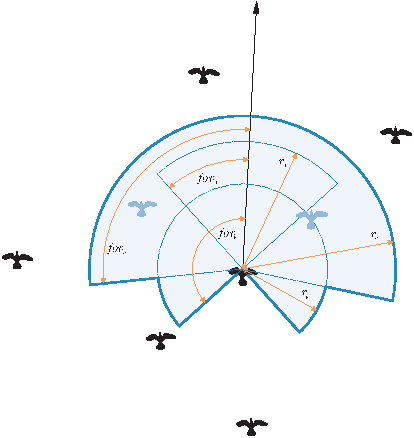
\includegraphics{fig_perception_cwr}
  \caption{The perception model that Reynolds used in the OpenSteer v0.8 implementation of his model \cite{reynolds:1999}. The black arrow represents the digital bird's flight direction. The shaded area represents the combined perception volume defined by the distinct separation ($r_\textnormal{s}$,$\fov_\textnormal{s}$), alignment ($r_\textnormal{a}$,$\fov_\textnormal{a}$) and cohesion ($r_\textnormal{c}$,$\fov_\textnormal{c}$) perception volumes. The perceived flockmates are depicted in a light blue colour.}
  \label{fig:perception:cwr}
\end{figure}

%-
\subsubsection{Modelling Perception}
As discussed before, in Reynolds's case, the universe is homogeneous (\ie\ consists of animats of the same kind). Furthermore, the number of animats is $n \in \N$ and constant through time. This means that the animat's input alphabet is $\set{X}=\set{Y}^n$.

Let $\set{Y}=\E \times \E$ and let the animat's output function $\lambda(q)=\langle\vect{p},\vect{v}\rangle$ return the animat's current position in space and its current velocity. Then at a discrete time step $t \in \set{T}$ the perceivable state of the universe is $u(t)=\langle y_1(t),\ldots,y_n(t)\rangle$, where for all $i=1,\ldots,n$ $y_i(t)=\lambda(q_i(t))$ is the output of animat $i$ (\ie\ its position in space and its velocity) at time step $t$.

As said, a perception function (definition~\ref{def:animat:Pi}) acts like an interpreter of the perceivable state of the universe and a selector of relevant information. Then, regarding the drives employed by Reynolds and the OpenSteer v0.8 source code, three perception functions $P_\textnormal{s}$, $P_\textnormal{a}$ and $P_\textnormal{c}$ must be defined. The separation perception function $P_\textnormal{s}$ returns the locations of the flockmates that must be avoided, the alignment perception function $P_\textnormal{a}$ returns the velocities of flockmates that should be followed and the cohesion perception function $P_\textnormal{c}$ returns the locations of flockmates that should be kept close to.

Let $\autom{B}_i$ and $\autom{B}_j$, where $i,j \in \N_n$, be two animats from Reynolds's digital universe and let $q_j=\langle\vect{p}_j,\vect{v}_j,s_j\rangle$ be the current state of animat $\autom{B}_j$ and $y_i=\lambda(q_i)=\langle \vect{p}_i,\vect{v}_i \rangle$ be the current output of animat $\autom{B}_i$ (\ie\ the perceivable data about it). Let $\autom{B}_j$ denote the observed animat. Then the distance of animat $\autom{B}_i$ is computed as
%
\begin{equation}
  \varepsilon_i=\left\|\vect{p}_i - \vect{p}_j\right\|, \label{eq:animat:cwr:distance}
\end{equation}
%
and the direction of the offset vector between them is computed as
%
\begin{equation}
  \varphi_i=\arccos \left( \frac {\vect{v}_j \cdot (\vect{p}_i - \vect{p}_j)}{\left\| \vect{v}_j \right\| \left\| \vect{p}_i - \vect{p}_j \right\|} \right). \label{eq:animat:cwr:angularOffset}
\end{equation}

\begin{definition}
  \label{def:animat:Ps:cwr}
  Let $x=\langle y_1,\ldots,y_n\rangle$ be the current perceivable state of the universe and $j$ the index of the observed animat. Let $\set{I}^\textnormal{s}=\E$ be the set representing obtainable information about a flockmate's location. Then $\set{P}^\textnormal{s}=\powset{\N_n} \times \E^n$ and equations~\eqref{eq:animat:Ps0:cwr}--\eqref{eq:animat:Ps2:cwr} define the \emph{separation perception function} $P_\textnormal{s}: \set{X} \times \set{Q} \mapsto \set{P}^\textnormal{s}$.
  \begin{eqnarray}
    & P_\textnormal{s}(x,q)=\langle\set{N}_\textnormal{s},o_\textnormal{s}\rangle, & \label{eq:animat:Ps0:cwr} \\
    & \set{N}_\textnormal{s}=\left\{i|\ i \in \N_n,\ i \neq j,\ \varepsilon_i%(q,y_i)
     \leq r_\textnormal{s},\ \varphi_i%(q,y_i)
     < \fov_\textnormal{s} \right\}, & \\
    & o_\textnormal{s}=\langle \vect{p}_1,\ldots,\vect{p}_n\rangle. & \label{eq:animat:Ps2:cwr}
  \end{eqnarray}
\end{definition}

\begin{definition}
  \label{def:animat:Pa:cwr}
  Let $x=\langle y_1,\ldots,y_n \rangle$ be the current perceivable state of the universe and $j$ the index of the observed animat. Let $\set{I}^\textnormal{a}=\E$ be the set representing obtainable information about a flockmate's velocity. Then $\set{P}^\textnormal{a}=\powset{\N_n} \times \E^n$ and equations~\eqref{eq:animat:Pa0:cwr}--\eqref{eq:animat:Pa2:cwr} define the \emph{alignment perception function} $P_\textnormal{a}: \set{X} \times \set{Q} \mapsto \set{P}^\textnormal{a}$.
  \begin{eqnarray}
    & P_\textnormal{a}(x,q)=\langle\set{N}_\textnormal{a},o_\textnormal{a}\rangle, & \label{eq:animat:Pa0:cwr} \\
    & \set{N}_\textnormal{a}=\left\{i|\ i \in \N_n,\ i \neq j,\ \varepsilon_i%(q,y_i)
     \leq r_\textnormal{a},\ \varphi_i%(q,y_i)
     < \fov_\textnormal{a}\right\}, & \\
    & o_\textnormal{a}=\langle \vect{v}_1,\ldots,\vect{v}_n\rangle. & \label{eq:animat:Pa2:cwr}
  \end{eqnarray}
\end{definition}

\begin{definition}
  \label{def:animat:Pc:cwr}
  Let $x=\langle y_1,\ldots,y_n \rangle$ be the current perceivable state of the universe and $j$ the index of the observed animat. Let $\set{I}^\textnormal{c}=\E$ be the set representing obtainable information about a flockmate's location. Then $\set{P}^\textnormal{c}=\powset{\N_n} \times \E^n$ and equations~\eqref{eq:animat:Pc0:cwr}--\eqref{eq:animat:Pc2:cwr} define the \emph{cohesion perception function} $P_\textnormal{c}: \set{X} \times \set{Q} \mapsto \set{P}^\textnormal{c}$.
  \begin{eqnarray}
    & P_\textnormal{c}(x,q)=\langle\set{N}_\textnormal{c},o_\textnormal{c}\rangle, & \label{eq:animat:Pc0:cwr} \\
    & \set{N}_\textnormal{c}=\left\{i|\ i \in \N_n,\ i \neq j,\ \varepsilon_i%(q,y_i)
     \leq r_\textnormal{c},\ \varphi_i%(q,y_i)
     < \fov_\textnormal{c}\right\}, & \\
    & o_\textnormal{c}=\langle \vect{p}_1,\ldots,\vect{p}_n\rangle. & \label{eq:animat:Pc2:cwr}
  \end{eqnarray}
\end{definition}

To sum up, the three perception functions together return only those digital birds that are in the perception volume of the observed digital bird. In other words, each of the three neighbourhoods represents only the flockmates that are treated as `nearby' according to the digital bird's corresponding drive \cite{reynolds:1987} (see subsection~\ref{subsec:birdFlocks:cwr}).

%-
\subsubsection{Modelling Drives}
Recall that a drive function (definition~\ref{def:animat:Dj}), based on the current perceived information about the state of the universe and the current state of the animat, selects the action to satisfy a specific drive. Then, since Reynolds states that flock-like behaviour can be achieved if the digital bird follows three drives, three drive functions $D_\textnormal{s}$, $D_\textnormal{a}$ and $D_\textnormal{c}$ need to be defined. The separation drive function $D_\textnormal{s}$ returns the action that will keep the animat safe from colliding with the flockmates which should be avoided. The alignment drive function $D_\textnormal{a}$ returns the action that will align it with the flockmates which should be followed and the cohesion drive function $D_\textnormal{c}$ returns the action that will direct it towards the centre of the flockmates which should be kept close to. Reynolds models the drives using geometrical equations (detailed descriptions are presented in \cite{reynolds:1999}) and since he models the digital bird as a simple vehicle \cite{reynolds:1987,reynolds:1999}, he represents the desired actions as physical forces which would induce the desired flight direction and/or flight speed change.

Let the animat's $k$-tuple of perception functions be  $P=\langle P_\textnormal{s},P_\textnormal{a},P_\textnormal{c}\rangle$. Then, according to definition~\ref{def:animat:Dj} and definitions~\ref{def:animat:Ps:cwr}--\ref{def:animat:Pc:cwr}, the set representing information obtainable from the perceivable state of the universe is $\set{P}=\set{P}^\textnormal{s} \times \set{P}^\textnormal{a} \times \set{P}^\textnormal{c}$.

According to Reynolds \cite{reynolds:1999}, the separation drive gives the digital bird the ability to maintain a certain separation distance from nearby flockmates. In this case the nearby flockmates are the digital birds that should be avoided (\ie\ computed using the separation perception function). For each flockmate a `repulsive force' is computed by subtracting the current position of the observed animat and the current position of the flockmate. This force is then divided by the square of the flockmate's distance.\footnote{Reynolds admits \cite{reynolds:1999} that the division by the square of the flockmate's distance is just a setting that worked well and not a fundamental value.} The resulting forces are then summed together, and according to \sidenote{OpenSteer v0.8}{!animats v1.0 should first average then normalize---opensteer does so!} also normalized, to produce the desired action (\ie\ the desired change in flight direction and flight speed).

\begin{definition}
  \label{def:animat:Ds:cwr}
  Let the current state of the animat be $q=\langle\vect{p},\vect{v},s\rangle$. Let the information that was, with respect to the current state of the animat $q$, obtained from the current perceivable state of the universe be $\langle p_\textnormal{s},p_\textnormal{a},p_\textnormal{c}\rangle \in \set{P}$ and let $p_\textnormal{s}=\langle\set{N}_\textnormal{s},o_\textnormal{s}\rangle$, where $\set{N}_\textnormal{s} \in \powset{\N_n}$ is a set representing the indexes of animats that should be avoided and $o_\textnormal{s}=\langle\vect{p}_1,\ldots,\vect{p}_n\rangle$ are their current positions in space. Let the set of available actions be $\set{A}=\E$. The \emph{separation drive function} is then the drive function $D_\textnormal{s}: \set{P} \times \set{Q} \mapsto \set{A}$ that is defined as
  \begin{equation}
    D_\textnormal{s}(\langle p_\textnormal{s},p_\textnormal{a},p_\textnormal{c}\rangle, q) = \left[ \sum_{i \in \set{N}_\textnormal{s}} \frac{\vect{p}-\vect{p}_i}{{\left\|\vect{p}_i-\vect{p}\right\|}^2} \right]^0. \label{eq:animat:Ds:cwr}
  \end{equation}
\end{definition}

The alignment drive, on the other hand, gives the digital bird the ability to align itself with (\ie\ fly in the same flight direction and/or with the same speed as) the nearby flockmates. The nearby flockmates in this case are the digital birds that should be followed. The average of the velocities of these flockmates is computed and represents the desired new velocity of the observed digital bird. The velocity difference is computed by subtracting the observed digital bird's velocity from the desired new velocity. Finally the force representing the desired action is then, according to OpenSteer v0.8, computed by normalizing the velocity difference.

\begin{definition}
  \label{def:animat:Da:cwr}
  Let the current state of the animat be $q=\langle\vect{p},\vect{v},s\rangle$. Let the information that was, with respect to the current state of the animat $q$, obtained from the current perceivable state of the universe be $\langle p_\textnormal{s},p_\textnormal{a},p_\textnormal{c}\rangle \in \set{P}$ and let $p_\textnormal{a}=\langle\set{N}_\textnormal{a},o_\textnormal{a}\rangle$, where $\set{N}_\textnormal{a} \in \powset{\N_n}$ is a set representing the indexes of animats that should be followed and $o_\textnormal{a}=\langle\vect{v}_1,\ldots,\vect{v}_n\rangle$ are their current velocities. Let the set of available actions be $\set{A}=\E$. The \emph{alignment drive function} is then the drive function $D_\textnormal{a}: \set{P} \times \set{Q} \mapsto \set{A}$ that is defined as
  \begin{equation}
    D_\textnormal{a}(\langle p_\textnormal{s},p_\textnormal{a},p_\textnormal{c}\rangle, q) = \left[ \Biggl( \frac{1}{\left|\set{N}_\textnormal{a}\right|} \sum_{i \in \set{N}_\textnormal{a}} \vect{v}_i \Biggr) - \vect{v} \right]^0. \label{eq:animat:Da:cwr}
  \end{equation}
\end{definition}

Finally, the cohesion drive gives the digital bird the ability to cohere with (\ie\ approach and form a group with) the nearby flockmates. Here the nearby flockmates are the digital birds that should be kept close to. The centre (\ie\ the \emph{centre of mass} or \emph{average position}) of these flockmates is computed and represents the desired position of the observed digital bird. The `attraction force' is computed by subtracting the observed digital bird's position from the desired position. At last the force representing the desired action is, according to OpenSteer v0.8, computed by normalizing the attraction force.

\begin{definition}
  \label{def:animat:Dc:cwr}
  Let the current state of the animat be $q=\langle\vect{p},\vect{v},s\rangle$. Let the information that was, with respect to the current state of the animat $q$, obtained from the current perceivable state of the universe be $\langle p_\textnormal{s},p_\textnormal{a},p_\textnormal{c}\rangle \in \set{P}$ and let $p_\textnormal{c}=\langle\set{N}_\textnormal{c},o_\textnormal{c}\rangle$, where $\set{N}_\textnormal{c} \in \powset{\N_n}$ is a set representing the indexes of animats that should be kept close to and $o_\textnormal{c}=\langle\vect{p}_1,\ldots,\vect{p}_n\rangle$ are their current positions in space. Let the set of available actions be $\set{A}=\E$. The \emph{cohesion drive function} is then the drive function $D_\textnormal{c}: \set{P} \times \set{Q} \mapsto \set{A}$ that is defined as
  \begin{equation}
    D_\textnormal{c}(\langle p_\textnormal{s},p_\textnormal{a},p_\textnormal{c}\rangle, q) = \left[ \left( \frac{1}{\left|\set{N}_\textnormal{c}\right|} \sum_{i \in \set{N}_\textnormal{c}} \vect{p}_i \right) - \vect{p} \right]^0. \label{eq:animat:Dc:cwr}
  \end{equation}
\end{definition}

%-
\subsubsection{Modelling Action Selection}
Each of the three drive functions returns a physical force that would satisfy the specific drive. Recall that the action selection function (definition~\ref{def:animat:S}), combines, prioritizes and arbitrates between potentially conflicting actions to select the sequence of muscular movements that will eventually accomplish all of the animal's drives. In his original study Reynolds \cite{reynolds:1987} proposes that the physical forces should be combined using a special algorithm named \emph{prioritized acceleration allocation}. But in one of his later studies \cite{reynolds:1999} he also admits that in the course of several reimplementations of the model over the years, a simpler linear combination has proved sufficient. Moreover, in his latest implementation in OpenSteer v0.8 he uses a weighted sum combination.

This means that Reynolds models action selection as a weighted sum of the desired actions (\ie\ weighted sum of the respective physical forces). The resulting force is used to compute the digital bird's new position in space and velocity. This computation is subjected to a set of constraints modelling conservation of momentum, viscous damping and the animal's finite amount of energy. He names the approach \emph{geometrical flight} \cite{reynolds:1987}.

\sidenote{Reynolds does not model the musculoskeletal structure of a bird}{v1.1.20050210 [FHH]: this may be a very unrealistic assumption---birds, like air planes, have stability-producing features that make them tend to go in a straight line unless positively directed otherwise.\\v1.3.20050402 [ILB]: This is taken care of by geometrical flight.}, but models it as a point mass vehicle \cite{reynolds:1987,reynolds:1999}. This means that the animat's physics is based on forward Euler integration. In other words, the combined forces (limited by the animat's maximal available force) are applied to the animat's point mass. This produces an acceleration equal to the combined force divided by the animat's mass. The acceleration is then added to the animat's current velocity and truncated by the maximum achievable speed. Finally the animat's new position in space is computed by adding the new velocity to the animat's current position in space.

Let $\vect{a} \in \E$ be a vector and let $a \in \R^+$ represent the maximal size of $\vect{a}$. Then the truncation of vector $\vect{a}$ to its maximal size $a$ is calculated as
%
\begin{equation}
  \lfloor\vect{a}\rceil^{a} = \min(\left\|\vect{a}\right\|, a) \vect{a}^0. \label{eq:truncation}
\end{equation}

\begin{definition}
  \label{def:animat:Sws:cwr}
  Let the current state of the animat be $q=\langle\vect{p},\vect{v},s\rangle$, where the modelled animal's internal state $s$ is defined by definition~\ref{def:animat:s:cwr}. Let the $l$-tuple of drive functions be $D=\langle D_\textnormal{s}, D_\textnormal{a}, D_\textnormal{c}\rangle$ and let the computed desired actions be $\langle a_\textnormal{s},a_\textnormal{a},a_\textnormal{c}\rangle$. Let $w_\textnormal{s}$, $w_\textnormal{a}$ and $w_\textnormal{c}$ represent the weights of the separation, alignment and cohesion drive respectively and let $dt$ represent the simulation step. Then the \emph{weighted sum action selection function} is the action selection function $S_\textnormal{ws}: \set{A} \times \set{Q} \mapsto \set{Q}$ that is defined as
  \begin{equation}
    S_\textnormal{ws}(\langle a_\textnormal{s},a_\textnormal{a},a_\textnormal{c}\rangle, q) = \langle\vect{p}', \vect{v}', s\rangle, \label{eq:animat:Sws0:cwr}
  \end{equation}
  \vspace{-3mm}
  \begin{equation}
    \vect{v}' = \left\lfloor {\vect{v} + \frac{\left\lfloor w_\textnormal{s}a_\textnormal{s} + w_\textnormal{a}a_\textnormal{a} + w_\textnormal{c}a_\textnormal{c} \right\rceil^{f_\textnormal{M}}}{m}}dt \right\rceil^{v_\textnormal{M}},
  \end{equation}
  \vspace{-3mm}
  \begin{equation}
    \vect{p}' = \vect{p} + \vect{v}'dt. \label{eq:animat:Sws2:cwr}
  \end{equation}
\end{definition}

Therefore Reynolds's digital bird can be defined as a special animat.

\begin{definition}
  \label{def:animat:cwr}
  Reynolds's digital bird is the animat $\autom{B}=\langle\set{X},\set{Q},\set{Y},\delta,\lambda,P,D,S\rangle$. The set representing internal states is $\set{Q}=\E \times \E \times \set{S}$, where $\set{S}$ is defined by definition~\ref{def:animat:s:cwr}. The output alphabet is $\set{Y}=\E \times \E$ and the input alphabet is $\set{X}=\set{Y}^n$. The animat's current internal state $q=\langle\vect{p},\vect{v},s\rangle$ represents the modelled animal's current position in space $\vect{p} \in \E$, velocity $\vect{v} \in \E$ and internal state $s \in \set{S}$. The output function $\lambda: \set{Q} \mapsto \set{Y}$ is $\lambda(q)=\langle\vect{p},\vect{v}\rangle$. The $k$-tuple of perception functions is $P=\langle P_\textnormal{s},P_\textnormal{a},P_\textnormal{c}\rangle$, where $P_\textnormal{s}$, $P_\textnormal{a}$ and $P_\textnormal{c}$ are the separation, alignment and cohesion perception function respectively (definitions~\ref{def:animat:Ps:cwr}--\ref{def:animat:Pa:cwr}). The $l$-tuple of drive functions is $D=\langle D_\textnormal{s},D_\textnormal{a},D_\textnormal{c}\rangle$, where $D_\textnormal{s}$, $D_\textnormal{a}$ and $D_\textnormal{c}$ are the separation, alignment and cohesion drive function respectively (definitions~\ref{def:animat:Ds:cwr}--\ref{def:animat:Dc:cwr}). Finally, the action selection function is the weighted sum action selection function $S=S_\textnormal{ws}$ (definition~\ref{def:animat:Sws:cwr}).
\end{definition}

%--
\subsection{Formalization of Heppner and Grenander's Computer Model}
\label{subsec:animat:fhh}
Heppner and Grenander in their study \cite{heppner:1990} modelled the universe as a collection of $n$ digital birds of the same kind. As a contrast to Reynolds they did not model any obstacles, but added a special influence modelling random distractions. Furthermore, they admit that without this influence they were not able to achieve flock-like behaviour.

Nevertheless, all things considered, they had a similar approach as Reynolds. Their digital bird moves through the universe with a certain velocity and at every discrete time step it changes this velocity in order to satisfy three drives: \emph{homing}, \emph{velocity regulation}, and \emph{interaction} (see subsection~\ref{subsec:birdFlocks:fhh}). The decision is again based purely on the digital bird's current state and the current perceivable state of the universe. More precisely the decision is based on the digital bird's position, velocity and the perceived locations of the nearby flockmates.

Let me define the animat that models Heppner and Grenander's digital bird. As discussed in section~\ref{sec:animat}, the animat's internal state $q \in \set{Q}$ is defined by the triplet $\langle \vect{p}, \vect{v}, s \rangle$, where $\vect{p} \in \E$ is its position in space, $\vect{v} \in \E$ its velocity and $s \in \set{S}$ is the modelled animal's internal state. Let me again first define the latter.

\begin{definition}
  \label{def:animat:s:fhh}
  Let $\vect{r} \in \E$ be the position of the centre of the roosting area of the the modelled bird, $r_\textnormal{o}$ its perception range, $v_\textnormal{p}$ its preferred flight speed and $d_\textnormal{p}$ its preferred distance from flockmates. Then the internal state of the animal modelled by Heppner and Grenander's digital bird is
  \begin{equation}
    s=\langle \vect{r}, r_\textnormal{o}, v_\textnormal{p}, d_\textnormal{p} \rangle.
  \end{equation}
\end{definition}

As in Reynold's case (subsection~\ref{subsec:animat:cwr}) I shall assume that only the animat's position $\vect{p}$ and $\vect{v}$ can change through time, while the 	modelled animal's internal state $s$ stays constant. This is again consistent with Heppner and Grenander's original definition \cite{heppner:1990}. The velocity vector $\vect{v}$ is thus again used to encode the flight direction $\vect{v}^0$ and flight speed $\left\|\vect{v}\right\|$. The perception range defines an omnidirectional perception volume (\fig~\ref{fig:perception:fhh}).

\begin{figure}
  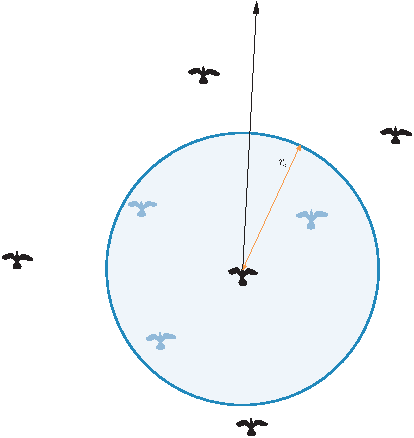
\includegraphics{fig_perception_fhh}
  \caption{The perception model used by Heppner and Grenander \cite{heppner:1990}. The black arrow represents the digital bird's flight direction. The shaded area represents the omnidirectional perception volume defined by the perception range. The perceived flockmates are depicted in a light blue colour.}
  \label{fig:perception:fhh}
\end{figure}

The preferred flight speed is the flight speed to which the bird wishes to return if perturbed and the preferred distance defines the optimal distance from a flockmate (\ie\ the distance at which the bird is neither attracted to nor repulsed from the flockmate).

%-
\subsubsection{Modelling Perception}
As discussed before, in Heppner and Grenander's case the universe again consists of animats of the same kind. Similarly, their number $n \in \N$ is constant through time, which means that the animat's input alphabet is yet again $\set{X}=\set{Y}^n$.

For reasons of consistency let the output alphabet again be $\set{Y}=\E \times \E$ and let the animat's output function $\lambda(q)=\langle\vect{p},\vect{v}\rangle$ return the animat's current position in space and velocity. Even in Heppner and Grenander's case the perceivable state of the universe at a discrete time step $t \in \set{T}$ is $u(t)=\langle y_1(t),\ldots,y_n(t)\rangle$, where for all $i=1,\ldots,n$ $y_i(t)=\lambda(q_i(t))$ is the output of animat $i$ (\ie\ its position in space and its velocity) at time step $t$.

Recall from subsection~\ref{subsec:birdFlocks:fhh} that Heppner and Grenander gave their digital bird full and precise knowledge about the locations of all surrounding digital birds that are closer than a predefined distance. Let $\autom{B}_i$ and $\autom{B}_j$, where $i, j \in \N_n$, be two animats from Heppner and Grenander's digital universe and let the current state of animat $\autom{B}_j$ be $q_j=\langle \vect{p}_j,\vect{v}_j,s_j \rangle$ and the current perceivable data about animat $\autom{B}_i$ be $y_i=\langle \vect{p}_i, \vect{v}_i \rangle$. Let $\autom{B}_j$ denote the observed animat. Then recall from equation~\eqref{eq:animat:cwr:distance} that the distance of animat $\autom{B}_i$ from the observed animat $\autom{B}_j$ is computed as
%
\begin{equation}
  \varepsilon_i=\left\|\vect{p}_i - \vect{p}_j\right\|. \nonumber
\end{equation}

\begin{definition}
  \label{def:animat:Po:fhh}
  Let $x=\langle y_1,\ldots,y_n\rangle$ be the current perceivable state of the universe and $j$ the index of the observed animat. Let $\set{I}^\textnormal{o}=\E$ be the set representing obtainable information about a flockmate's location. Then $\set{P}^\textnormal{o}=\powset{\N_n} \times \E^n$ and equations~\eqref{eq:animat:Po0:fhh}--\eqref{eq:animat:Po2:fhh} define the \emph{omnidirectional perception function} $P_\textnormal{o}: \set{X} \times \set{Q} \mapsto \set{P}^\textnormal{o}$.
  \begin{eqnarray}
    & P_\textnormal{o}(x,q)=\langle\set{N}_\textnormal{o},o_\textnormal{o}\rangle, & \label{eq:animat:Po0:fhh} \\
    & \set{N}_\textnormal{o}=\left\{i|\ i \in \N_n,\ i \neq j,\ \varepsilon_i \leq r_\textnormal{o} \right\}, & \\
    & o_\textnormal{o}=\langle \vect{p}_1,\ldots,\vect{p}_n\rangle. & \label{eq:animat:Po2:fhh}
  \end{eqnarray}
\end{definition}

%-
\subsubsection{Modelling Drives}
Recall from subsection~\ref{subsec:birdFlocks:fhh} that homing expresses the bird's tendency to stay in a roosting area and depends only on the digital bird's current position. Velocity regulation expresses its tendency to fly with a certain flight speed and depends only on the digital bird's current flight speed. Finally interaction expresses the bird's attraction to or repulsion from flockmates and depends only on the perceived locations of the nearby flockmates.

Let the animat employ only the omnidirectional perception function. Then $P=\langle P_\textnormal{o} \rangle$ and, according to definitions~\ref{def:animat:Dj} and \ref{def:animat:Po:fhh}, the set representing information obtainable from the perceivable state of the universe is $\set{P}=\set{P}^\textnormal{o}$.

\begin{definition}
  \label{def:animat:Dh:fhh}
  Let the current state of the animat be $q=\langle\vect{p},\vect{v},s\rangle$, where the modelled animal's internal state is $s=\langle\mathrm{r},r_\textnormal{o},v_\textnormal{p},d_\textnormal{p}\rangle$ as defined by definition~\ref{def:animat:s:fhh}. Let $p_\textnormal{o}$ denote the neighbourhood obtained by using the omnidirectional perception function. Let the set of available actions be $\set{A}=\E$. Let $h_\textnormal{m}$ be the minimum distance for roost attraction and $h_\textnormal{M}$ the distance of maximum roost attraction. The \emph{homing drive function} is then the drive function $D_\textnormal{h}: \set{P} \times \set{Q} \mapsto \set{A}$ that is defined as
  \begin{equation}
    D_\textnormal{h}(p_\textnormal{o}, q) = \left\{
    \begin{array}{ll}
    \vect{0} & \mathrm{iff}\ \left\|\vect{r}-\vect{p}\right\| < h_\textnormal{m} \\
    \frac{c^a \mathrm{e}^{-bc}}{\left(a/b\right)^a \mathrm{e}^{-a}} \left(\vect{r}-\vect{p}\right)^0  & \mathrm{iff}\ \left\|\vect{r}-\vect{p}\right\| \geq h_\textnormal{m}
    \end{array}
    \right., \label{eq:animat:Dr:fhh}
  \end{equation}
  where $a$ and $b$ are parameters for controlling the shape of the attraction function and
  \begin{equation}
    c=\frac{a}{b}\left(\frac{\left\|\vect{r}-\vect{p}\right\|-h_\textnormal{m}}{h_\textnormal{M}}\right).
  \end{equation}
\end{definition}

\begin{definition}
  \label{def:animat:Dv:cwr}
  Let the current state of the animat be $q=\langle\vect{p},\vect{v},s\rangle$, where the modelled animal's internal state is $s=\langle\mathrm{r},r_\textnormal{o},v_\textnormal{p},d_\textnormal{p}\rangle$ as defined by definition~\ref{def:animat:s:fhh}. Let $p_\textnormal{o}$ denote the neighbourhood obtained by using the omnidirectional perception function and let the set of available actions be $\set{A}=\E$. The \emph{velocity regulation drive function} is then the drive function $D_\textnormal{v}: \set{P} \times \set{Q} \mapsto \set{A}$ that is defined as
  \begin{equation}
    D_\textnormal{v}(p_\textnormal{o}, q) = \left(v_\textnormal{p}-\left\|\vect{v}\right\|\right)\vect{v}^0. \label{eq:animat:Dv:fhh}
  \end{equation}
\end{definition}

\begin{definition}
  \label{def:animat:Di:fhh}
  Let the current state of the animat be $q=\langle\vect{p},\vect{v},s\rangle$, where the modelled animal's internal state is $s=\langle\mathrm{r},r_\textnormal{o},v_\textnormal{p},d_\textnormal{p}\rangle$ as defined by definition~\ref{def:animat:s:fhh}. Let the neighbourhood obtained by using the omnidirectional perception function be $p_\textnormal{o}=\langle\set{N}_\textnormal{o},o_\textnormal{o}\rangle$, where $\set{N}_\textnormal{o} \in \powset{\N_n}$ is the set of indexes of relevant animats and $o_\textnormal{o}=\langle\vect{p}_1,\ldots,\vect{p}_n\rangle$ are their locations. Let the set of available actions be $\set{A}=\E$ and let $f_\textnormal{M}$ denote the maximal repulsion force. The \emph{interaction drive function} is then the drive function $D_\textnormal{i}: \set{P} \times \set{Q} \mapsto \set{A}$ that is defined as
  \begin{equation}
    D_\textnormal{i}(p_\textnormal{o}, q) = \sum_{i \in \set{N}_\textnormal{o}} \left[1-\frac{(\left\|\vect{p}_i-\vect{p}\right\|-a)^2}{b}\right] c \left(\vect{p}_i-\vect{p}\right)^0, \label{eq:animat:Di:fhh}
  \end{equation}
  where $a=\frac{d_\textnormal{p}+r_\textnormal{o}}{2}$, $b=\left(\frac{d_\textnormal{p}-r_\textnormal{o}}{2}\right)^2$ and
  \begin{equation}
    c = \left\{
    \begin{array}{ll}
      1 & \mathrm{iff}\ \left\|\vect{p}_i-\vect{p}\right\| \geq d_\textnormal{p} \\
      \left\|\vect{p}_i-\vect{p}\right\|\frac{(b-a^2)-f_\textnormal{M}}{d_\textnormal{p}(b-a^2)}+\frac{f_\textnormal{M}b}{b-a^2} & \mathrm{iff}\ \left\|\vect{p}_i-\vect{p}\right\| < d_\textnormal{p}
    \end{array}
    \right..
  \end{equation}
\end{definition}

%-
\subsubsection{Modelling Action Selection}
Each of the three drive functions returns a vector which may be interpreted as an unconventional (non-Newtonian) \cite{heppner:1990} force that would satisfy the specific drive. Recall that the action selection function (definintion~\ref{def:animat:S}) combines, prioritizes and arbitrates between these potentially conflicting forces. Heppner and Grenander again took a similar approach as Reynolds and modelled action selection as a simple weighted sum. However, apart from the Poisson stochastic process modelling the effects of wind gusts and random local disturbances they did not apply any additional constraints.

\begin{definition*}
  \label{def:animat:Ss:fhh}
  Let the current state of the animat be $q=\langle\vect{p},\vect{v},s\rangle$. Let the $l$-tuple of drive functions be $D=\langle D_\textnormal{h}, D_\textnormal{v}, D_\textnormal{i}\rangle$ (definitions~\ref{def:animat:Dh:fhh}--\ref{def:animat:Di:fhh}) and let the computed desired actions be $\langle a_\textnormal{h},a_\textnormal{v},a_\textnormal{i}\rangle$. Let $w_\textnormal{h}$, $w_\textnormal{v}$ and $w_\textnormal{i}$ represent the weights of the homing, velocity regulation and interaction drive respectively and let $dt$ represent the simulation step. Then the \emph{simple weighted sum action selection function} is the action selection function $S_\textnormal{s}: \set{A} \times \set{Q} \mapsto \set{Q}$ that is defined as
  \begin{eqnarray}
    & S_\textnormal{s}(\langle a_\textnormal{h},a_\textnormal{v},a_\textnormal{i}\rangle, q) = \langle\vect{p}', \vect{v}', s\rangle, & \label{eq:animat:Ss0:fhh} \\
    & \vect{p}' = \vect{p} + \vect{v}dt, & \\
    & \vect{v}' = \vect{v} + \left(w_\textnormal{h}a_\textnormal{h} + w_\textnormal{v}a_\textnormal{v} + w_\textnormal{i}a_\textnormal{i}\right)dt + \vect{d}dt, & \label{eq:animat:Ss2:fhh}
  \end{eqnarray}
  where $\vect{d} \in \E$ is a Poisson controlled vector modelling random distractions.
\end{definition*}

Heppner and Grenander's digital bird \cite{heppner:1990} is therefore a special animat.

\begin{definition}
  \label{def:animat:fhh}
  The animat modelling Heppner and Grenander's digital bird is the animat $\autom{B}=\langle\set{X},\set{Q},\set{Y},\delta,\lambda,P,D,S\rangle$. The set representing internal states is $\set{Q}=\E \times \E \times \set{S}$, where $\set{S}$ is defined by definition~\ref{def:animat:s:fhh}. The output alphabet is $\set{Y}=\E \times \E$ and the input alphabet is $\set{X}=\set{Y}^n$. The animat's current internal state $q=\langle\vect{p},\vect{v},s\rangle$ represents the modelled animal's current position in space $\vect{p} \in \E$, velocity $\vect{v} \in \E$ and internal state $s \in \set{S}$. The output function $\lambda: \set{Q} \mapsto \set{Y}$ is $\lambda(q)=\langle\vect{p},\vect{v}\rangle$. The $k$-tuple of perception functions is $P=\langle P_\textnormal{o}\rangle$, where $P_\textnormal{o}$ is the omnidirectional perception function (definition~\ref{def:animat:Po:fhh}). The $l$-tuple of drive functions is $D=\langle D_\textnormal{h},D_\textnormal{v},D_\textnormal{i}\rangle$, where $D_\textnormal{h}$, $D_\textnormal{v}$ and $D_\textnormal{i}$ are the homing, velocity regulation and interaction drive function respectively (definitions~\ref{def:animat:Dh:fhh}--\ref{def:animat:Di:fhh}). The action selection function is the simple weighted sum action selection function $S=S_\textnormal{s}$ (definition~\ref{def:animat:Ss:fhh}).
\end{definition}

 	% !TeX root = ./thesis.tex










%==============================
\chapter{Fuzzy Modelling}
\label{ch:fuzzyModelling}


%-----
\section{Fuzzy Sets}
\label{sec:fuzzyModelling:fuzzySets}
Fuzzy sets are a natural outgrowth and generalization of conventional (or crisp) sets. Recall that a \emph{crisp set} in a \emph{universe of discourse} (\ie\ a collection of objects that represents allowable values for a variable) can be defined by stating all of its members or by specifying the \emph{precise properties} required for membership. 

Take for example the set of real numbers `from 3 to 5' and denote it as $\set{C}$. In this case the universe of discourse is the set of real numbers $\R$ and $\set{C}$ is a crisp set. It can be described by writing $\set{C}=\{r \in \R| 3 \leq r \leq 5\}$. 

Equivalently, a crisp set can be described by specifying its \emph{membership function} that maps from the universe of discourse to the set $\{0,1\}$. The membership function returns 1 for all objects from the universe of discourse that satisfy the required properties and 0 for those that do not. 

In the case of the crisp set $\set{C}$ the membership function returns 1 for all real numbers that satisfy the property `from 3 to 5' and 0 for all other (\fig~\ref{fig:fuzzy:set}a). If $\mu_\set{C}$ is used to denote the membership function of crisp set $\set{C}$, then $\forall r \in \R$:
%
\begin{equation}
	\mu_\set{C}(r)=\left\{
	 \begin{array}{ll}
	   1, & \mathrm{if\ }3 \leq r \leq 5 \\
	   0, & \mathrm{otherwise}.
	 \end{array}
	\right.
\end{equation}

Fuzzy sets, on the contrary, contain elements that satisfy \emph{imprecisely defined properties} \cite{bezdek:1992}. Zadeh \cite{zadeh:1965} proposed describing them by using a generalized membership function that maps from the universe of discourse to the entire unit interval $[0,1]$. This is the basic idea in fuzzy set theory; the membership function provides the degree to which an object from the universe of discourse satisfies the imprecisely defined properties \cite{bezdek:1992}. It provides the object's \emph{degree of membership}. 

Take for example the `set' of real numbers that are `close to 4'. Because the property `close to 4' is imprecise, the `set' of real numbers that are `close to 4' is a fuzzy set. Let it be denoted by $\fset{F}$. Again the universe of discourse is the set of real numbers $\R$, but the membership function $\mu_\fset{F}$ now provides the degree of membership of a real number in the fuzzy set $\fset{F}$; the nearer the value of $\mu_\fset{F}(r)$ to unity, the higher the degree of membership of $r$ in $\fset{F}$. This means that $\mu_\fset{F}(r)$ provides the measure of the degree of consistency between $r$ and the interpretation of `close to 4'. 

However, since the property `close to 4' is imprecise and its interpretation subjective, there is not a unique membership function for $\fset{F}$. Rather, it is left to the modeller to decide what $\mu_\fset{F}$ should be like. In this particular case, with respect to the property `close to 4', it seems plausible that:

\begin{itemize}
	\item the degree of membership of number $4$ is unity, 
	\item the closer a number is to $4$, the closer its degree of membership is to unity,
	\item numbers equally far left and right of $4$ have equal memberships.
\end{itemize}

\begin{figure*}
	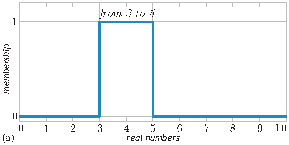
\includegraphics[width=\figurewidth/2-1mm]{fig_fuzzySet_a}\hspace*{2mm}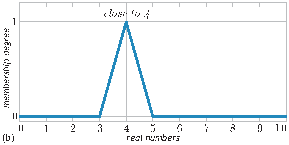
\includegraphics[width=\figurewidth/2-1mm]{fig_fuzzySet_b}
	\caption{Membership functions of a crisp set of real numbers `from 3 to 5' (a) and a fuzzy set of real numbers `close to 4' (b).}
	\label{fig:fuzzy:set}
\end{figure*}

Given these intuitive constraints, a useful representation of the fuzzy set of numbers `close to 4' might be the fuzzy set $\fset{F}$ that is presented in \fig~\ref{fig:fuzzy:set}b and described by the membership function
%
\begin{equation}
\mu_\fset{F}(r)=\max(0,1-|r-4|).
\end{equation} 

Recall that in crisp set theory the family of \emph{all crisp sets} that can be defined in a given universe of discourse $\set{X}$ is called the \emph{power set} of $\set{X}$, and is usually denoted by $\powset{\set{X}}$. Thus, returning to the examples, it can be written that $\set{C} \in \powset{\R}$. 

Similarly, in fuzzy set theory, the family of \emph{all fuzzy sets} that can be defined in a given universe of discourse $\set{X}$ is called the \emph{fuzzy power set} of $\set{X}$, and is usually denoted by $\fpowset{\set{X}}$ \cite{klir:1995}. Therefore, again returning to the examples, it can be written that $\fset{F} \in \fpowset{\R}$.

%--
\subsection{Set Theoretic Operations for Fuzzy Sets}
In order to manipulate fuzzy sets, Zadeh \cite{zadeh:1965} generalized the classical set theoretic operations (\ie\ intersection, union and complement) and introduced \emph{fuzzy intersection}, \emph{fuzzy union}, and \emph{fuzzy complement}. 

\begin{definition}
Let fuzzy sets $\fset{F}_1$ and $\fset{F}_2$, defined on the universe of discourse $\set{X}$, be described by their membership functions $\mu_{\fset{F}_1}$ and $\mu_{\fset{F}_2}$. The fuzzy set theoretic operations are then defined using the following operators:

\begin{itemize}
	\item fuzzy intersection:
	  \begin{itemize}
	    \item \emph{minimum}:  $\mu_{\fset{F}_1 \cap \fset{F}_2}(x)=\min(\mu_{\fset{F}_1}(x),\mu_{\fset{F}_2}(x))$,
	    \item \emph{algebraic product}:  $\mu_{\fset{F}_1 \aprod \fset{F}_2}(x)=\mu_{\fset{F}_1}(x)\cdot\mu_{\fset{F}_2}(x)$,
	  \end{itemize}
	
	\item fuzzy union:
	  \begin{itemize}
	    \item \emph{maximum}:  $\mu_{\fset{F}_1 \cup \fset{F}_2}(x)=\max(\mu_{\fset{F}_1}(x),\mu_{\fset{F}_2}(x))$,
	    \item \emph{algebraic sum}:  $\mu_{\fset{F}_1 \uplus \fset{F}_2}(x)=\mu_{\fset{F}_1}(x)+\mu_{\fset{F}_2}(x)-\mu_{\fset{F}_1}(x)\cdot\mu_{\fset{F}_2}(x)$,
	  \end{itemize}
	
	\item fuzzy complement:  
	  $\mu_{\overline{\fset{F}_1}}(x)=1-\mu_{\fset{F}_1}(x)$.
\end{itemize}
\end{definition}

The minimum fuzzy intersection, maximum fuzzy union and fuzzy complement are also known under the names standard fuzzy intersection, standard fuzzy union and standard fuzzy complement. Later Klir and Yuan \cite{klir:1995} showed that by using a strong axiomatic basis many more operators can be defined. They even gave an axiomatic definition for the complement of a fuzzy set, but in engineering applications most people prefer to use the standard fuzzy complement defined by Zadeh \cite{zadeh:1965}.  


%-----
\section{Fuzzy Logic}
\label{subsec:fuzzyModelling:fuzzyLogic}
The membership function of a crisp set maps real numbers to two values (0 or 1). Hence crisp sets correspond to conventional (crisp or two-valued) logic. Logic works with \emph{statements}. Take for example the statement `\fvar{distance} \kwd{is} \fval{from 3 to 5}'. It can be either \emph{true} or \emph{false}; there is no ambiguity in it. Let $d$ denote the value of \fvar{distance} and $\set{C}$ denote the set of numbers `from 3 to 5'. Then the question of this statement's \emph{truth} becomes a question of membership `is $d$ in $\set{C}$?' and the answer is true if $\mu_\set{C}(d)=1$ and false if $\mu_\set{C}(d)=0$. 

On the other hand, the value of $\mu_\fset{F}(r)$ provides the degree of membership of $r$ in fuzzy set $\fset{F}$. Therefore fuzzy sets correspond to continuously valued logic. Take for example the statement `\fvar{distance} \kwd{is} \fval{close to 4}'. Because `close to 4' is an imprecisely defined property, this statement is not crisp at all; it cannot be told if it is true or false. However, a similar approach as in two-valued logic can be used, the value of \fvar{distance} denoted by $d$, but `close to 4' defined as a fuzzy set $\fset{F}$. Then the question of the statement's truth becomes again a question of membership `is $d$ in $\fset{F}$?' but the value $\mu_\fset{F}(d)$ now answers the statement's \emph{degree of truth}. The answer can be true ($\mu_\fset{F}(d)=1$), false ($\mu_\fset{F}(d)=0$) or anywhere in between ($0<\mu_\fset{F}(d)<1$). 

Furthermore, in fuzzy logic the value of \fvar{distance} can be a fuzzy set too. Let it be denoted as $\fset{D}$. The statement's truth now becomes a question of \emph{similarity} `is $\fset{D}$ similar to $\fset{F}?$' and the answer is given by the highest degree of membership of objects that are common to both fuzzy sets (\ie\ $\sup_r\mu_{\fset{D} \cap \fset{F}}(r)$).

Logic allows joining simple statements to form more complex ones. This is achieved through standard logical operators, namely `\kwd{and}', `\kwd{or}', and `\kwd{not}'. An example of a complex crisp statement is `(\fvar{distance} \kwd{is} \fval{from 3 to 5}) \kwd{and} (\fvar{speed difference} \kwd{is} \fvar{20\,m/s})'. 

Evaluating such statements involves computing the truths of the substatements and applying the logical operators. In two-valued logic the compound statement is true: 

\begin{itemize}
	\item when all of the substatements are true (logical operator `\kwd{and}'), 
	\item when at least one of the substatements is true (logical operator `\kwd{or}'), 
	\item when the substatement is false (logical operator `\kwd{not}').
\end{itemize}

However, in fuzzy logic the constraint of the absolute truth or falsity of a statement is relaxed and this influences the interpretation of logical operators. Nevertheless, as fuzzy logic is a superset of standard two-valued logic, if the degrees of truth are kept at the extremes of 1 (completely true), and 0 (completely false), standard logical operators will hold. The most common interpretation is to use the operators that Zadeh \cite{zadeh:1965} used to define fuzzy intersection (logical operator `\kwd{and}'), fuzzy union (logical operator `\kwd{or}'), and fuzzy complement (logical operator `\kwd{not}'). In other words this means that to resolve the truth of the statement `$\statement{A}$ \kwd{and} $\statement{B}$', where $\statement{A}$ and $\statement{B}$ are statements and $T(\statement{A})$, $T(\statement{B})$ denote their corresponding degrees of truth, the following function is evaluated
%
\begin{itemize}
	\item $T(\statement{A}\ \kwd{and}\ \statement{B})=\min(T(\statement{A}),T(\statement{B}))$ (\ie\ minimum fuzzy intersection),
	\item $T(\statement{A}\ \kwd{and}\ \statement{B})=T(\statement{A}) \cdot T(\statement{B})$ (\ie\ algebraic product fuzzy intersection),
\end{itemize}
%
similarly the degree of truth of `$\statement{A}$ \kwd{or} $\statement{B}$' becomes equivalent 
%
\begin{itemize}
	\item $T(\statement{A}\ \kwd{or}\ \statement{B})=\max(T(\statement{A}),T(\statement{B}))$ (\ie\ maximum fuzzy union),
	\item $T(\statement{A}\ \kwd{or}\ \statement{B})=T(\statement{A}) + T(\statement{B}) - T(\statement{A}) \cdot T(\statement{B})$ (\ie\ algebraic sum fuzzy union),
\end{itemize}
%
and finally, the degree of truth of `\kwd{not} $\statement{A}$' is computed as 
%
\begin{itemize}
	\item $T(\kwd{not}\ \statement{A})=1 - T(\statement{A})$ (\ie\ standard fuzzy complement).
\end{itemize}

Typically most fuzzy logic applications make use of these operators. But any combination of fuzzy union, fuzzy intersection and fuzzy complement operators can be used as far as it is made sure that either DeMorgan's laws are not used or that fuzzy union and fuzzy intersection are dual with respect to the chosen fuzzy complement \cite{klir:1995}. This means that the different operators that are available in fuzzy set theory provide a plethora of richness, but also some (tough) choices have to be made \cite{mendel:2001}. In this dissertation the logical operator `\kwd{and}' is interpreted as product fuzzy intersection, the logical operator `\kwd{or}' as maximum fuzzy union and `\kwd{not}' as the standard fuzzy complement.

%--
\subsection{The if-then Rule}
\label{subsec:fuzzyModelling:ifthen}
Logic makes often use of a special statement known as \emph{if-then} rule, which assumes the form `\kwd{if} $\statement{A}$ \kwd{then} $\statement{C}$', where $\statement{A}$ and $\statement{C}$ are statements. The if-part of the rule (\ie\ statement $\statement{A}$) is called the \emph{antecedent} or premise, while the then-part (\ie\ statement $\statement{C}$) is called the \emph{consequent} or conclusion. The antecedent can always be written as a set of statements connected with the logical operator `\kwd{and}' \cite{mendel:2001}, which means that the rule can be read as a set of \emph{conditions} that must be met for a certain consequence. However, this also means that antecedents of if-then rules that have the same conclusion can be joined using the logical operator `\kwd{or}' and interpreted as a single if-then rule. 

Interpreting an if-then rule involves evaluating the truth of the antecedent and applying that result to the consequent (known as \emph{implication}). In the case when the antecedent has multiple parts, their degrees of truth are calculated simultaneously and the truth of the antecedent is resolved by applying the logical operators. In two-valued logic the interpretation of the if-then rule is simple. Whenever the premise is true the conclusion is true too. However, if the premise is false nothing can be said about the conclusion. Since in fuzzy logic the truth of the antecedent is a matter of degree, the interpretation of the if-then rule is less restricted. This means that whenever the antecedent is true to some degree, the consequent is also true to that same degree. 

However, because in fuzzy logic the consequent specifies a fuzzy set to be assigned to the output, implication modifies this set to the degree specified by the antecedent. The most common ways to modify the output fuzzy set are chopping it off (\ie\ \emph{minimum fuzzy implication}) or squashing it (\ie\ \emph{product fuzzy implication}). Let $T(\statement{A})$ denote the antecedent's degree of truth and $\fset{F}$ be the output fuzzy set defined on the real numbers domain. Let $\mu_\fset{F}$ denote the membership function of the output fuzzy set and $\mu_{\fset{F}'}$ the membership function of the modified output fuzzy set. Then minimum fuzzy implication is computed as
%
\begin{equation} 
	\mu_{\fset{F}'}(r)=\min(T(\statement{A}),\mu_\fset{F}(r))
\end{equation}
%
and product fuzzy implication as
%
\begin{equation}
	\mu_{\fset{F}'}(r)=T(\statement{A})\cdot\mu_\fset{F}(r).
\end{equation}

\begin{figure}
	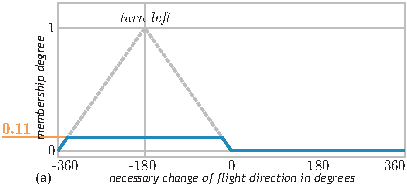
\includegraphics{fig_fuzzyImplication_a}\\
	\vspace*{2mm}
	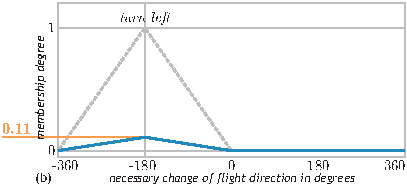
\includegraphics{fig_fuzzyImplication_b}
	\caption{Graphical representation of the minimum (a) and product (b) fuzzy implication. The dashed grey line represents the original output fuzzy set while the blue solid line represents the modified output fuzzy set.}
	\label{fig:implication}
\end{figure}

Take for example the if-then rule whose consequent is `\fvar{direction} \kwd{is} \fvar{turn left}' and let the degree of truth of its antecedent be $T(\statement{A})=0.11$. The minimum fuzzy implication's effect of chopping off the output fuzzy set can be seen in \fig~\ref{fig:implication}a while the squashing effect of the product fuzzy implication can be seen in \fig~\ref{fig:implication}b. 

\subsection{The Fuzzy Rule Base}
\label{subsec:fuzzyModelling:fuzzyRuleBase}
Rarely the output of a decision process can be described by a single if-then rule. On the contrary; in most cases it is described by a collection of if-then rules, which are in fuzzy logic usually called a \emph{fuzzy rule base}. In addition: in fuzzy logic individual rules from a fuzzy rule base can at times be mutually contradictive. 

In two-valued logic with a given input value usually the antecedent of only one rule is true. This means that the output value is at all times unequivocally known. However, as in fuzzy logic the interpretation of if-then rules is less restricted and mutually contradictive rules are allowed, more than one rule's antecedent can be true to some degree. This means that after applying fuzzy logic on a fuzzy rule base, one ends up with a collection of modified output fuzzy sets which represent only candidates for the final output value. 

Most fuzzy logic applications solve this by \emph{combining} the modified output fuzzy sets into a single fuzzy set, which thereon represents the final output value of the fuzzy rule base. In most cases this combination is done by computing the fuzzy union of the modified output fuzzy sets. 

The final output value of the fuzzy rule base is thus represented by the combined fuzzy set. However, as in most cases the fuzzy rule base is used as a control decision process, and the controlled process usually requires crisp control inputs, the fuzzy rule base's output (\ie\ the combined fuzzy set) needs to be converted to a single (crisp) value \cite{klir:1995,mendel:2001}. This conversion is called \emph{defuzzification}. For a given fuzzy set it returns the single (crisp) value which, in some sense, is the best representative of the fuzzy set.

A number of defuzzification methods leading to distinct results were proposed in literature \cite{dubois:1980,klir:1995,mendel:2001,pedrycz:1993,zimmermann:2001}, but the most commonly used, and also the one used in this dissertation, is called the \emph{centroid} method. In this method, which is sometimes called the \emph{centre of gravity} or \emph{centre of area} method, the defuzzified value is defined as the crisp value, for which the area under the graph of the membership function of the combined fuzzy set is divided into two equal subareas (\fig~\ref{fig:cog}). 

Let $\fset{F} \in \fpowset{\R}$ denote the combined fuzzy set obtained by evaluating a fuzzy rule base and let $\mu_\fset{F}$ represent its membership function. Then the centroid defuzzified value is calculated as
\begin{equation}
	\cog\fset{F}=\frac{\int r \mu_\fset{F}(r)\mathrm{d}r}{\int\mu_\fset{F}(r)\mathrm{d}r}.
\end{equation}

\begin{figure}
	\vspace*{5mm}
	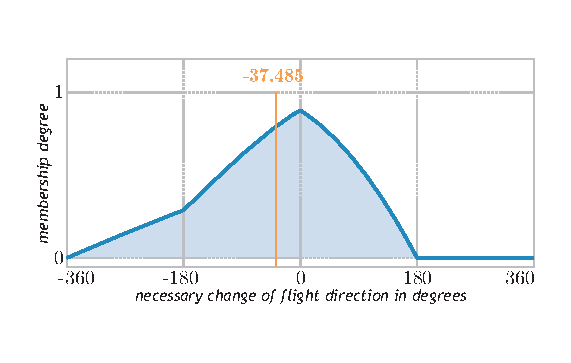
\includegraphics{fig_cog}
	\vspace*{5mm}
	\caption{Graphical representation of the centroid defuzzification. The blue line represents the membership function of the final output value of a fuzzy rule base computed by combining the output fuzzy sets of individual fuzzy rules. The orange line divides the area under the graph of the membership function (shaded area) into two equal subareas and thus represents the single (crisp) value that is, according to the centroid defuzzification method, the best representative of the combined fuzzy set.}
	\label{fig:cog}
\end{figure}

	% !TeX root = ./thesis.tex










%==============================
\chapter{The Fuzzy Animat}
\label{ch:fuzzyAnimat}


%----
\section{The Fuzzy Digital Animal}
\label{sec:fuzzyAnimat}
Modelling organized groups of moving animals is a complex task, requiring thorough knowledge about the behaviour of the modelled animal. However, the behavioural repertoire displayed by animals is typically so large that even ethologists are at times unable to form hypotheses about the actions guiding the displayed behaviour, not to mention the reasons that initiated it. Exact knowledge is thus usually not available, and in cases when knowledge is available, it usually cannot be truth-tested.

Furthermore, the linguistic descriptions and explanations of the perceived behaviour generally bear a fair amount of influence by the observer and are consequently uncertain or ambiguous per se. Knowledge about animal behaviour can as a consequence be best described as uncertain, ambiguous or fuzzy. This is where fuzzy logic, with its ability to model using uncertain knowledge and process uncertain data, shows its potential. In this chapter I shall thus introduce fuzziness into the animat (see \chaptername~\ref{ch:animat}) and with this allow constructing digital animals using uncertain, ambiguous or fuzzy knowledge.

Recall that, at the most basic level, the universe is a collection of inanimate and animate objects. This dissertation assumes that the perceivable state of the universe can be represented as a crisp value. In other words, I assume that data about objects constituting the universe that can be perceived by an outside observer is crisp. This seems reasonable. After all, taking for example a tree in the nearby park; even though its exact size cannot be perceived or described it could be measured, provided there was an infinitely precise measurement aid.

In addition, I also assume that the objects constituting the universe update their states in parallel, at discrete time steps, and that the method of updating is local, however not necessarily homogeneous. Therefore, regardless of the method employed for constructing the digital animals the digital universe can be represented as a collection of animats whether they are fuzzy or not.

Let me concentrate on the introduction of fuzziness into the animat. Recall first that the animat (definition~\ref{def:animat}) is an extended Moore automaton, taking into account a certain set of animal characteristic (\ie\ perception, drives, action selection). Recall also that the digital universe is a collection of $n$ animats. This means that the perceivable state of the universe at a discrete time step $t \in \set{T}$ is given by the $n$-tuple $u(t)=\langle y_1(t),\ldots,y_n(t)\rangle$, where $y_i(t)=\lambda(q_i(t))$ is the output of animat $i$ at time step $t$, for all $i=1,\ldots,n$. In addition, recall that at a discrete time step $t \in \set{T}$ all animats are applied the same input (\ie\ the current perceivable state of the universe). Thus $x(t)=u(t)$ and the input alphabet is $\set{X}=\set{U}=\set{Y}_1 \times \cdots \times \set{Y}_n$. Finally, recall that the state of animat $i$ at a discrete time step $t \in \set{T}$ is, in most cases when modelling organised groups of moving animals, given as $q_i(t)=\langle \vect{p}_i(t), \vect{v}_i(t), s_i(t) \rangle$, where $\vect{p}_i(t) \in \E$ denotes its position in space, $\vect{v}_i(t) \in \E$ its velocity and $s_i(t) \in \set{S}_i$ the internal state of the modelled animal. In other words, the above states that the animats' fuzziness originates from their decision processing (\ie\ perception, drives and action selection).

\begin{definition}
  \label{def:fuzzyAnimat}
  A fuzzy animat $\fautom{A}=\langle\set{X},\set{Q},\set{Y},\delta,\lambda,\ffunc{P},\ffunc{D},\ffunc{S}\rangle$ is an extended Moore automaton, where $\ffunc{P}=\langle\ffunc{P}_1,\ldots,\ffunc{P}_k\rangle$ is a $k$-tuple of fuzzy perception functions, $\ffunc{D}=\langle\ffunc{D}_1,\ldots,\ffunc{D}_l\rangle$ is an $l$-tuple of fuzzy drive functions, $\ffunc{S}$ is a fuzzy action selection function and the transition function $\delta$ is defined as:
  \begin{eqnarray}
    & \delta(x,q) = \ffunc{S}(\langle\fset{A}_1,...,\fset{A}_l\rangle,q), & \label{eq:fuzzyAnimat:delta}\\
    & \fset{A}_j = \ffunc{D}_j(\langle\fset{P}_1,...,\fset{P}_k\rangle,q),\ j=1,\ldots,l, & \\
    & \fset{P}_i = \ffunc{P}_i(x,q),\ i=1,\ldots,k. & \label{eq:fuzzyAnimat:Pi}
  \end{eqnarray}
\end{definition}

If I sum up, at a discrete time step even the fuzzy animat is applied the current perceivable state of the universe (\ie\ the crisp data about all of the animats, fuzzy or not,\footnote{Indeed the universe can be a mixed collection of crisp and fuzzy animats. Due to this the term animat shall be used, throughout the rest of this dissertation, to address both animat versions (\ie\ the fuzzy and crisp).} that can be observed by an outside observer). Using the transition function (\ie\ taking into account fuzzy perception, fuzzy drives and fuzzy action selection) it then computes the next discrete time step state and emits its new output, which as a consequence changes the perceivable state of the universe. The following sections discuss fuzzy perception, fuzzy drives and fuzzy action selection in more detail.

%--
\subsection{Fuzzy Perception}
As discussed before, the input of a fuzzy animat is the current perceivable state of the universe. Recall that the crisp perception function (definition~\ref{def:animat:Pi}) is used to model the animal's process of interpreting the perceivable data and selecting just the relevant information from all of the sensory signals that exist in the universe. However, the crisp perception function allows modelling only accurate perception (\ie\ one that gives the animat exact knowledge about the state of the universe). As we know from our own perception of the world, the latter is `unnatural'. A fuzzy perception function, which allows modelling inaccurate perception as well, should therefore be defined.

Let the current perceivable state of the universe be the $n$-tuple $u=\langle y_1,\ldots,y_n \rangle$, where for all $i=1,\ldots,n$ $y_i$ is data about animat $i$ that can be perceived by an outside observer. Let $q \in \set{Q}$ be the current state of the observed fuzzy animat and let its input $x \in \set{X}$ be the current perceivable state of the universe $x=\langle y_1,\ldots,y_n \rangle$.

Recall that $\N_n$ denotes the set of all positive natural numbers lower or equal to $n$ and for all $i=1,\ldots,n$ $\set{I}^\textnormal{c}_i$ represents information about animat $i$ that can be obtained from $y_i$ with respect to a certain characteristic $\mathrm{c}$.

Let $\fset{N} \in \fpowset{\N_n}$ represent the fuzzy set of indexes of members of $x$ (\ie\ animats) that are according to characteristic $\mathrm{c}$ vaguely relevant to the observed fuzzy animat. As a contrast to the crisp perception function, where an animat can only be relevant or irrelevant, the relevancy is now a matter of degree. The ordered pair $\langle\fset{N},\fset{O}\rangle$, where $\fset{N} \in \fpowset{\N_n}$ and $\fset{O} \in \fpowset{\set{I}^\textnormal{c}_1} \times \cdots \times \fpowset{\set{I}^\textnormal{c}_n}$ represents uncertain information regarding characteristic $\mathrm{c}$ that was obtained from the current perceivable state of the universe and is, with respect to this characteristic, vaguely relevant to the observed fuzzy animat. For reasons of simplicity the same approach as in the crisp perception function will be employed and $\fpowset{\N_n} \times (\fpowset{\set{I}^\textnormal{c}_1} \times \cdots \times \fpowset{\set{I}^\textnormal{c}_n})$ will be denoted simply as $\fpowset{\set{P}^\textnormal{c}}$.\footnote{In fact, in this dissertation, when $\set{X}=\set{X}_1 \times \cdots \times \set{X}_m$, I use $\fpowset{\set{X}}$ to denote $\fpowset{\set{X}_1} \times \cdots \times \fpowset{\set{X}_m}$ and not $\fpowset{\set{X}_1 \times \cdots \times \set{X}_m}$.}

\begin{definition}
  \label{def:fuzzyAnimat:Pi}
  Let $x \in \set{X}$ be the current perceivable state of the universe and $\fset{P} \in \fpowset{\set{P}^\textnormal{c}}$ be the uncertain information regarding characteristic $\mathrm{c}$ that was obtained from $x$ and is, according to this characteristic and the state $q \in \set{Q}$, vaguely relevant to the animat. Then a \emph{fuzzy perception function} for characteristic $\mathrm{c}$ is a mapping $\ffunc{P}: \set{X} \times \set{Q} \mapsto \fpowset{\set{P}^\textnormal{c}}$.
\end{definition}

For reasons of simplicity I shall address the image of a fuzzy perception function with the name \emph{fuzzy neighbourhood}. Relating to the crisp perception function this means that the fuzzy neighbourhood represents only the vaguely relevant and inaccurately characterized sensory signals (\eg\ inaccurate locations of uncertain food sources).

%--
\subsection{Fuzzy Drives}
Recall that the crisp drive function (definition~\ref{def:animat:Dj}) is used to model the process with which, based on the information obtained from the perceivable state of the universe and its current internal state, the animal selects the action that satisfies a certain drive. Since the fuzzy animat perceives the universe inaccurately and knowledge about the animal's drives is usually vague, the drive function should take this into account.

Let the observed fuzzy animat have $k$ fuzzy perception functions. Let them be denoted as $\ffunc{P}_1,\ldots,\ffunc{P}_k$. This means that $\fpowset{\set{P}}=\fpowset{\set{P}^{\mathrm{c}_1}} \times \cdots \times \fpowset{\set{P}^{\mathrm{c}_k}}$ represents uncertain information obtainable from the current perceivable state of the universe. For all $i=1,\ldots,k$ let $\fset{P}_i \in \fpowset{\set{P}^{\mathrm{c}_i}}$ denote the fuzzy neighbourhood that was obtained with perception function $\ffunc{P}_i$. Then $\langle \fset{P}_1,\ldots,\fset{P}_k \rangle \in \fpowset{\set{P}}$ represents the perceived uncertain information about the current state of the universe that was, with respect to the current state of the fuzzy animat, obtained from the current perceivable state of the universe.

\begin{definition}
  \label{def:fuzzyAnimat:Dj}
  Let $\set{A}$ denote the set of all possible actions of the fuzzy animat. Let the uncertain action that, with respect to the perceived uncertain information about the current state of the universe $\langle \fset{P}_1,\ldots,\fset{P}_k \rangle \in \fpowset{\set{P}}$ and the current state of the fuzzy animat $q \in \set{Q}$, satisfies a specific, vaguely known, drive be represented by the fuzzy set $\fset{A} \in \fpowset{\set{A}}$. Then a \emph{fuzzy drive function} is a mapping $\ffunc{D}: \fpowset{\set{P}} \times \set{Q} \mapsto \fpowset{\set{A}}$.
\end{definition}

The studied animal's drives are in the case of the crisp animat  usually implemented through mathematical equations (\eg\ digital birds by Reynolds \cite{reynolds:1987,reynolds:1999}---subsection~\ref{subsec:animat:cwr} and Heppner and Grenander \cite{heppner:1990}---subsection~\ref{subsec:animat:fhh}). In addition, as discussed, exact knowledge about the studied animal's behaviour is rarely available. Indeed, it is usually available only in the form of descriptions of the observed behaviour bearing a fair amount of influence by the observer, and transition from such descriptions to mathematical equations is far from straightforward. The fuzzy drive functions of the fuzzy animat, on the other hand, because of their use of fuzzy logic, allow the studied animal's drives to be implemented using collections of if-then rules. This makes the transition from descriptions to drive functions much simpler and the construction of digital animals much easier. In addition the requirement for exact knowledge is removed.

%--
\subsection{Fuzzy Action Selection}
Bring to mind that the crisp action selection function (definition~\ref{def:animat:S}) is used to model the neurological process of selecting the sequence of muscular movements that will accomplish the actions that result from the animal's drives and combines, prioritizes and arbitrates between potentially conflicting actions. Since in the case of the fuzzy animat the actions are uncertain, the action selection function has to take this into account. This section shall thus define the fuzzy action selection function.

Let the observed fuzzy animat have $l \in \N$ fuzzy drive functions $\ffunc{D}_1,\ldots,\ffunc{D}_l$. Then the $l$-tuple $\langle \fset{A}_1,\ldots,\fset{A}_l \rangle \in \fpowset{\set{A}}^l$ represents the fuzzy animat's desired uncertain actions.

\begin{definition}
  \label{def:fuzzyAnimat:S}
  Let $q' \in \set{Q}$ denote the next state of the fuzzy animat computed by taking into account the current state of the animat $q \in \set{Q}$ and combining, prioritizing and arbitrating between its desired uncertain actions $\langle \fset{A}_1,\ldots,\fset{A}_l \rangle \in \fpowset{\set{A}}^l$. Then a \emph{fuzzy action selection function} is a mapping $\ffunc{S}: \fpowset{\set{A}}^l \times \set{Q} \rightarrow \set{Q}$.
\end{definition}

If I sum up, the three stage scheme of the fuzzy animat's transition function, as in the case of the crisp animat, imitates the adopted theory about animal behaviour (\fig~\ref{fig:animat}). The first stage is used to model the studied animal's perception of the universe, the second stage to model its drives and finally the third stage to model the process of selecting and executing the sequence of muscular movements that will eventually satisfy its drives. However, as a contrast to the crisp animat, the fuzzy animat's fuzzy perception, fuzzy drive and fuzzy action selection functions allow constructing a model of an animal even by using only vague knowledge about its behaviour.


%----
\section{Case Study}
\label{sec:fuzzyAnimat:afd}
The previous section presented a formal definition of the fuzzy animat. The latter can be used to model inanimate or animate objects by using ambiguous knowledge and data. In this section I shall use it to construct a fuzzy model for a computer simulation of bird flocking. More precisely, it will be used to construct a fuzzy digital bird.

Recall that Reynolds \cite{reynolds:1987} (subsection~\ref{subsec:animat:cwr}) modelled the universe as a collection of animats of same kind and obstacles that represented inanimate objects. Similarly, recall that Heppner and Grenander \cite{heppner:1990} (subsection~\ref{subsec:animat:fhh}), on the other hand, modelled the universe as a collection of animats of same kind and excluded inanimate objects, but added a special influence which is intended to simulate the effects of wind gusts and random local disturbances. Furthermore, they state that in their case the latter was of crucial importance for flock-like behaviour \cite{heppner:1990}.

Since I am interested in producing a self-organizing flight flock, I employ the same approach and model the universe as a collection of $n$ fuzzy animats. What is more, at this stage I also omit obstacles. I justify the omission with the fact that natural flocks form and exist also in open spaces, where there are no obstacles. For the time being I also do not simulate the effects of wind gusts and random local disturbances, even though it would be interesting to test the effect of their inclusion, which I plan as part of my future research. In addition I take the same approach as Reynolds \cite{reynolds:1987,reynolds:1999} and Heppner and Grenander \cite{heppner:1990} and assume a constant universe (\ie\ even though the animats' states change through time their number stays constant).

As discussed in section~\ref{sec:fuzzyAnimat}, the fuzzy animat's internal state $q \in \set{Q}$ is defined by the triplet $\langle \vect{p}, \vect{v}, s \rangle$, where $\vect{p} \in \E$ is its position in space, $\vect{v} \in \E$ its velocity and $s \in \set{S}$ is the modelled animal's internal state.

\begin{definition}
  \label{def:fuzzyAnimat:s:afd}
  Let $r_\textnormal{v}$ be the range of the modelled bird's visual perception, $\fov_\textnormal{v}$ its per eye visual field and $b_\textnormal{v}$ the angle of binocular overlap. Let $m$ represent the modelled bird's mass, $v_\textnormal{M}$ its maximal achievable flight speed and $f_\textnormal{M}$ its maximal available force. Then
  \begin{equation}
    s=\langle r_\textnormal{v}, \fov_\textnormal{v}, b_\textnormal{v}, m, v_\textnormal{M}, f_\textnormal{M} \rangle.
  \end{equation}
\end{definition}

As when constructing Reynolds's digital bird (subsection~\ref{subsec:animat:cwr}), I shall assume that only the fuzzy animat's position $\vect{p}$ and velocity $\vect{v}$ change through time, while the modelled animal's internal state $s$ stays constant. The velocity vector $\vect{v}$ again gives the fuzzy animat's relative position changes per coordinate axis in the Cartesian coordinate system and therefore encodes the fuzzy animat's flight direction $\vect{v}^0$ and flight speed $\left\|\vect{v}\right\|$. The visual perception range, per eye visual field and the angle of binocular overlap define the animat's perception volume (\ie\ they will be used to model visual perception). In addition, the maximal achievable speed represents a simple model of viscous speed damping (\ie\ it will be used to model the inability to exceed a certain speed even if constantly accelerating), while the maximal available force will be used to take into account the fact that an animal with a finite amount of energy is being modelled.

\begin{definition}
  \label{def:fuzzyAnimat:afd}
  My fuzzy digital bird is $\fautom{B}=\langle\set{X},\set{Q},\set{Y},\delta,\lambda,\ffunc{P},\ffunc{D},\ffunc{S}\rangle$, a fuzzy animat (definition~\ref{def:fuzzyAnimat}). The set representing its internal states is $\set{Q}=\E \times \E \times \set{S}$, where $\set{S}$ is defined by definition~\ref{def:fuzzyAnimat:s:afd}. The output alphabet is $\set{Y}=\E \times \E$ and the input alphabet is $\set{X}=\set{Y}^n$. The fuzzy animat's current internal state $q=\langle\vect{p},\vect{v},s\rangle$ represents the modelled animal's current position in space $\vect{p} \in \E$, velocity $\vect{v} \in \E$ and internal state $s \in \set{S}$. The output function $\lambda: \set{Q} \mapsto \set{Y}$ is $\lambda(q)=\langle\vect{p},\vect{v}\rangle$. The $k$-tuple of fuzzy perception functions is $\ffunc{P}=\langle\ffunc{P}_\textnormal{v}\rangle$, where $\ffunc{P}_\textnormal{v}$ is the fuzzy visual perception function (definition~\ref{def:fuzzyAnimat:Pv:afd}). The $l$-tuple of fuzzy drive functions $\ffunc{D}=\langle\ffunc{D}_\textnormal{a},\ffunc{D}_\textnormal{r},\ffunc{D}_\textnormal{p}\rangle$, where $\ffunc{D}_\textnormal{a}$, $\ffunc{D}_\textnormal{r}$ and $\ffunc{D}_\textnormal{p}$ are the fuzzy attraction, fuzzy repulsion and fuzzy alignment drives respectively  (definitions~\ref{def:fuzzyAnimat:Da:afd}--\ref{def:fuzzyAnimat:Dp:afd}). The fuzzy action selection function is the fuzzy weighted sum action selection function $\ffunc{S}=\ffunc{S}_\textnormal{ws}$ (definition~\ref{def:fuzzyAnimat:Sws:afd}).
\end{definition}

In the following sections I shall discuss the fuzzy visual perception function, the fuzzy attraction, fuzzy repulsion, and fuzzy alignment drives, as well as the fuzzy weighted sum action selection, in more detail.

%--
\subsection{Modelling Visual Perception}
As discussed in subsections~\ref{subsec:birdFlocks:fhh} and \ref{subsec:animat:fhh} Heppner and Grenander \cite{heppner:1990} give each animat complete and precise information about the universe. In doing so they make an unrealistic assumption because real birds have limited and inaccurate perceptive capabilities (\eg\ nearby flockmates hide those far away, thus the bird cannot visually perceive them). Reynolds \cite{reynolds:1987}, on the other hand, as discussed in subsections~\ref{subsec:birdFlocks:cwr} and \ref{subsec:animat:cwr}, admitting that a bird's perception of the world is severely limited by occlusion, models perception as a volume within which the animat has the ability to sense flockmates. But in his case the sensed information is precise---giving the animat precise information about the state of its flockmates (\ie\ their exact distance, position, flight speed and flight direction). Even though Reynolds \cite{reynolds:1987} states that his perception model tries to make available approximately the same information that is available to a bird as the end result of perceptual and cognitive processes, his approach, although better, is still unrealistic. A bird's visual perception is not limited only by occlusion, but also by the fact that the ability to sense distance, apart from being \sidenote{affected by the degree of binocular overlap,}{v1.3.20050407 [FHH]: Binocular vision may not be as important as you suggest for depth perception. Cover one eye, and try to pick up a pencil off a desk. You will probably very good at it. Simply shifting the head slightly will give a different view, which gives you the depth.} decreases with distance itself.

Even though it is likely that aerodynamic perception is as important in birds as hydrodynamic perception is important in fish \cite{ward:2001}, I currently model only visual perception. Although it is still an unrealistic model, I adopt a slightly modified Reynolds's \cite{reynolds:1999} approach of localized visual perception. The main difference between the two is in the returned information.

In fact, I model visual perception as a visual volume defined by the visual range $r_\textnormal{v}$, per eye visual field $\fov_\textnormal{v}$ and the angle of binocular overlap $b_\textnormal{v}$ of the fuzzy animat (see \fig~\ref{fig:perception:afd}).
%
\begin{figure}
  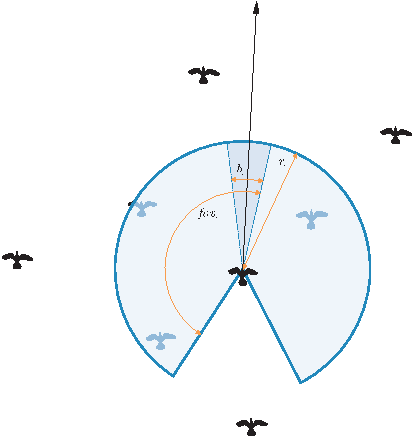
\includegraphics{fig_perception_afd}
  \caption{The perception model used in my fuzzy animat. The black arrow represents the fuzzy digital bird's flight direction. The shaded area represents the visual volume defined by the visual range $r_\textnormal{v}$, per eye visual field $\fov_\textnormal{v}$ and the angle of binocular overlap $b_\textnormal{v}$. The perceived flockmates are depicted in a light blue colour.}
  \label{fig:perception:afd}
\end{figure}
%
At the time being I am using the visual range of seven body lengths and the per eye visual field of \ang{150} with no binocular overlap so that the fuzzy animat has a blind area of \ang{60} behind it, which corresponds closely to the values reported by Heppner \etal\ \cite{heppner:1985}. However, instead of giving full information about the perceived flockmates I give only their \emph{distance}, \emph{angular offset}, relative \emph{difference in flight speed} and relative \emph{difference in flight direction}. I justify this by the fact that using visual perception, a bird can sense only the distance and angular offset of a flockmate, but through cognitive processes and tracking it can judge the relative difference in flight speed (\ie\ if the flockmate is moving faster, slower or with the same speed) and their relative difference in flight direction (\ie\ if the flockmate is flying more to the left, more to the right or in the same direction). Nevertheless in my current implementation the sensed information is still precise (\ie\ exact distance, angular offset, \etc).\footnote{It could be argued that by using this information one can calculate the same precise information as in Reynolds's \cite{reynolds:1999} case, but I strongly object to any mentioning that a bird has precise or full information about its global position in space, absolute flight speed or absolute flight direction.} I reserve the modelling of the binocular overlap and inaccurate visual perception for future work.

Recall that, as in Reynolds's case, in my case the digital universe is homogeneous. Indeed it consists of $n$ fuzzy animats of same kind denoted as $\fautom{B}_1,\ldots,\fautom{B}_n$. Recall that my fuzzy animat's output function is also $\lambda(q)=\langle \vect{p}, \vect{v} \rangle$, where $\vect{p} \in \E$ is the animat's current position in space and $\vect{v} \in \E$ its velocity. This means that at a discrete time step $t \in \set{T}$ the perceivable state of the universe is $u(t)=\langle y_1(t),\ldots,y_n(t) \rangle$, where for all $i=1,\ldots,n$ $y_i=\lambda(q_i(t))$ is the output of fuzzy animat $\fautom{B}_i$ at time step $t$.

As a crisp perception function a fuzzy perception function acts like an interpreter of the perceivable state of the universe and selector of relevant information. But as a contrast to the crisp version it allows modelling inaccurate perception. However, as already said, in the current implementation I model visual perception as accurate.

Let $\fautom{B}_i$ and $\fautom{B}_j$, where $i, j \in \N_n$, be two fuzzy animats from the digital universe and let $q_j=\langle \vect{p}_j, \vect{v}_j, s_j \rangle$ be the current state of fuzzy animat $\fautom{B}_j$ and $y_i=\lambda(q_i)=\langle \vect{p}_i, \vect{v}_i \rangle$ the current output of fuzzy animat $\fautom{B}_i$. Let $\fautom{B}_j$ denote the observed animat. Recall from equation~\eqref{eq:animat:cwr:distance} that the crisp distance of fuzzy animat $\fautom{B}_i$ can be computed as
%
\begin{equation}
  \varepsilon_i=\left\|\vect{p}_i - \vect{p}_j\right\|,
\end{equation}
%
and from equation~\eqref{eq:animat:cwr:angularOffset} that the direction of the offset vector between them (\ie\ their crisp angular offset) can be computed as
%
\begin{equation}
  \varphi_i=\arccos \left( \frac {\vect{v}_j \cdot (\vect{p}_i - \vect{p}_j)}{\left\| \vect{v}_j \right\| \left\| \vect{p}_i - \vect{p}_j \right\|} \right).
\end{equation}

The crisp difference in flight speed between the observed fuzzy animat $\fautom{B}_j$ and fuzzy animat $\fautom{B}_i$ is on the other hand computed as
%
\begin{equation}
  \varsigma_i=\left\|\vect{v}_i\right\| - \left\|\vect{v}_j\right\|.
\end{equation}

As already said, the velocity vector $\vect{v}$ gives the relative position changes per coordinate axis in the Cartesian coordinate system. Let $\vect{a}_\textnormal{x}$, $\vect{a}_\textnormal{y}$ and $\vect{a}_\textnormal{z}$ denote the $\mathrm{x}$, $\mathrm{y}$ and $\mathrm{z}$ axis components of vector $\vect{a}$. Then since I am using a two-dimensional Euclidean space $\E=\R^2$, where $\vect{a} \times \vect{b} = \vect{a}_\textnormal{x}\vect{b}_\textnormal{y} - \vect{a}_\textnormal{y}\vect{b}_\textnormal{x}$, the crisp difference in flight direction between the observed fuzzy animat $\fautom{B}_j$ and fuzzy animat $\fautom{B}_i$ is computed as
%
\begin{equation}
  \vartheta_i=\sgn\left(\vect{v}_i \times \vect{v}_j\right)\arccos \left( \frac {\vect{v}_i \cdot \vect{v}_j}{\left\| \vect{v}_i \right\| \left\| \vect{v}_j \right\|} \right),
\end{equation}
%
where $\sgn: \R \mapsto \R$ is the \emph{signum function} defined as
\begin{equation}
  \sgn x=\left\{
  \begin{array}{rl}
  -1 & \mathrm{iff}\ x < 0\\
  0 & \mathrm{iff}\ x = 0\\
  1 & \mathrm{iff}\ x > 0
  \end{array}
  \right..
\end{equation}

In my model of visual perception the observed animat perceives only the distance, angular offset, difference in flight speed and difference in flight direction of the fuzzy animats that are in its visual volume. This means that the set of visually obtainable information about a fuzzy animat is $\set{I}^\textnormal{v}=\R^4$ and the fuzzy neighbourhood is $\langle\fset{N},\fset{O}\rangle$, where $\fset{N} \in \fpowset{\N_n}$ and $\fset{O} \in \fpowset{\set{I}^\textnormal{v}}^n$. However, since in the current implementation the perception is accurate, the fuzzy set $\fset{N}$ is in fact a crisp set $\set{N} \in \N_n$ and $\fset{O}$ is a crisp value $o \in {(\set{I}^\textnormal{v})}^n$.\footnote{Indeed this can safely be done because fuzzy sets are a generalization of crisp sets and a crisp set $\set{A}$ defined on the universe of discourse $\set{X}$ can always be represented as the fuzzy set $\fset{A}$ whose membership function $\mu_\fset{A}(x)=1\ \mathrm{iff}\ x \in \set{A}$ and $\mu_\fset{A}(x)=0\ \mathrm{iff}\ x \notin \set{A}$, for all $x \in \set{X}$.}

\begin{definition}
  \label{def:fuzzyAnimat:Pv:afd}
  Let $x=\langle y_1,\ldots,y_n\rangle$ be the current perceivable state of the universe, $j$ denote the index of the observed fuzzy animat and let $\set{I}^\textnormal{v}=\R^4$ be the set representing visually obtainable information about a flockmate's distance, angular offset, difference in flight speed and difference in flight direction. Then $\fpowset{\set{P}^\textnormal{v}}=\fpowset{\N_n} \times \fpowset{\set{I}^\textnormal{v}}^n$ and equations~\eqref{eq:fuzzyAnimat:Pv0:afd}--\eqref{eq:fuzzyAnimat:Pv2:afd} define the \emph{fuzzy visual perception function} $\ffunc{P}_\textnormal{v}: \set{X} \times \set{Q} \mapsto \fpowset{\set{P}^\textnormal{v}}$.
  \begin{eqnarray}
    & \ffunc{P}_\textnormal{v}(x,q)=\langle\fset{N},\fset{O}\rangle, & \label{eq:fuzzyAnimat:Pv0:afd} \\
    & \fset{N}=\left\{i|\ i \in \N_n,\ i \neq j,\ \varepsilon_i%(q,y_i)
     \leq r_\textnormal{v},\ \varphi_i%(q,y_i)
     < \fov_\textnormal{v} \right\}, & \\
    & \fset{O}=\langle \langle \varepsilon_1, \varphi_1, \varsigma_1, \vartheta_1 \rangle, \ldots,
    \langle \varepsilon_n, \varphi_n, \varsigma_n, \vartheta_n \rangle \rangle. & \label{eq:fuzzyAnimat:Pv2:afd}
  \end{eqnarray}
\end{definition}

%--
\subsection{Modelling Drives}
Even though, as discussed in subsections~\ref{subsec:birdFlocks:cwr} and \ref{subsec:animat:cwr}, Reynolds in his latest studies \cite{reynolds:1999,reynolds:2000} presented drives\footnote{In his papers he uses the name steering behaviours, but for reasons of consistency and clarity the term drives is used throughout this dissertation.} through the combination of which one can achieve complex behaviours, he states that flocking behaviour can be achieved using only three drives, namely \emph{separation}, \emph{alignment} and \emph{cohesion}. Cohesion simulates attraction toward flockmates and is modelled as the animat's tendency to fly towards the centre of mass of the perceived flockmates. Separation simulates repulsion away from flockmates and is modelled as the animat's tendency to fly away from the perceived flockmates. These two drives (cohesion and separation) represent the attraction-repulsion scheme. Alignment, on the other hand, tries to produce polarization and is modelled as the animat's tendency to change its flight direction and flight speed, so that it corresponds to the average flight direction and flight speed of its perceived flockmates.

Heppner and Grenander \cite{heppner:1990} (subsections~\ref{subsec:birdFlocks:fhh} and \ref{subsec:animat:fhh}) also modelled three, but different, drives, namely \emph{homing}, \emph{velocity regulation} and \emph{interaction}. Homing simulates the attraction of the roosting point and is modelled as the animat's tendency to fly toward the roosting point. This tendency drops to zero if the animat is close enough (\ie\ a predefined distance) or too far away (\ie\ a predefined distance) from the roosting point. Velocity regulation is modelled as the animat's tendency to fly at a certain predefined preferred speed. Interaction, on the other hand, combines the attraction-repulsion scheme in one single drive and simulates the actual interaction between animats. If two animats are too close (\ie\ a predefined distance) they are repelled, if they are too far (\ie\ a predefined distance) they do not influence each other and if they are anywhere in between, they are attracted.

Attraction towards and repulsion from the flockmates feel natural. After all, their mutual coexistence and importance for the congregation's structure has already been suggested by Okubo \cite{okubo:1980}. Another important feature of groups of uniform density is polarization \cite{parrish:1997a}. Heppner and Grenander \cite{heppner:1990} did not model it specifically, but they mention that in certain cases organized flocks maintaining straight direction of flight emerged. This might be caused by the perception model they used (\ie\ all animats have complete and accurate information about the universe) in conjunction with the velocity regulation drive. Reynolds \cite{reynolds:1987}, however, tries to model polarization through the drive of alignment.

According to the above discussion I model these three primary drives, the \emph{attraction to flockmates} (fuzzy attraction drive), the \emph{repulsion from flockmates} (fuzzy repulsion drive) and \emph{polarization with flockmates} (fuzzy alignment drive). In the following subsections I will discuss them in greater detail. Note that when modelling attraction to flockmates I do not use a predefined preferred position like the centre of mass \cite{reynolds:1987} and similarly, when modelling polarization with flockmates I do not use a predefined preferred flight speed \cite{heppner:1990}. Instead I let these properties emerge on their own.

As said before, my fuzzy animat perceives the current state of the universe through visual perception only. At any point in time the fuzzy animat perceives only information about a localized subset of the universe. Since I model the universe as a collection of fuzzy animats, the fuzzy animat thus perceives information about its nearby flockmates. The perceived information includes only distance, angular offset, relative difference in flight direction and relative difference in flight speed of the nearby flockmates. At the time being the perceived information is precise and I reserve modelling inaccurate perception for future work. In addition, I shall suppose that the fuzzy animat can act only by changing its flight speed and/or flight direction.

%-
\subsubsection{The Fuzzy Attraction Drive}
The primary motive of the attraction drive is to stay close to nearby neighbours. Now, imagine a bird that perceives only one neighbour. How would you, in the simplest way possible, describe the action that will keep it close to the perceived neighbour? Assuming that the bird can act only by changing its flight speed and/or flight direction and using common sense most of us would probably state the following:
\begin{enumerate}
  \item in general do not change flight speed or flight direction; \label{dscr:attraction}
  \item when the perceived neighbour is `close enough', change neither flight speed nor flight direction;
  \item when the perceived neighbour is `too far' and `in front', speed up;
  \item when the perceived neighbour is `too far' and anywhere to the `left or behind', turn toward it and slow down;
  \item when the perceived neighbour is `too far' and anywhere to the `right or behind', turn toward it and slow down.
\end{enumerate}

Looking carefully at this description, it can be noticed that the resulting action depends only on the perceived neighbour's distance (\ie\ `close enough', `too far') and position (\ie\ `in front', `left or behind', `right or behind'). But what do `close enough', `too far', `in front', \etc\ mean? Does `in front' perhaps address the precise moment when the perceived neighbour is positioned at an angular offset of \ang{0}? What about \ang{5}, is the perceived neighbour then not `in front'? As it can be seen, `in front' is an imprecise property and constructing a mathematical model from a description that builds on such imprecise properties is a challenging task, which usually requires advanced mathematical skills. Then again, because `close enough', `too far', `in front', \etc\ are imprecise properties and do not represent \emph{crisp values} like \ang{0} or \ang{5}, they can be labelled as vague or \emph{fuzzy values}. Thanks to Zadeh \cite{zadeh:1965}, who introduced \emph{fuzzy sets} (see section~\ref{sec:fuzzyModelling:fuzzySets}), such values can be formally defined.\footnote{In fact, according to the latest fuzzy sets related literature \cite{lee:2004} a fuzzy value is a fuzzy set defined in the real number domain.} Constructing the attraction drive now becomes simple. All that needs to be done is to rewrite the description as a collection of easily understandable \emph{if-then rules} (subsection~\ref{subsec:fuzzyModelling:ifthen}) and the necessary action can be afterwards computed by applying \emph{fuzzy logic} (subsection~\ref{subsec:fuzzyModelling:fuzzyLogic}).

Consider, for example, the fuzzy value `close enough'. As already said, it can be represented with a fuzzy set. In other words, this means that a fuzzy value is uniquely defined by its membership function. In this case, the latter provides the degree to which a real number satisfies the property `close enough' (\ie\ its degree of membership). But because the interpretation of `close enough' is subjective, there is no unique membership function; it is left to the modeller to decide what it should be like. Thus the question is: what did we have in mind with `close enough'? I shall assume that the perceived neighbour is considered as `close enough' if its distance is 40\% of the visual range or less. As the distance increases, the perceived neighbour is considered less and less `close enough' and eventually, when it gets out of the visual range, it is not considered as `close enough' at all. \sidenote{This translates in the membership function that is presented on \fig~\ref{fig:fuzzyAnimat:Da:afd}a.}{v1.1.20050210 [FHH]: these could be explained in more detail for biologists.}
%
\begin{figure}
  \null\vspace*{2mm}\par
  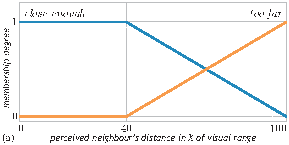
\includegraphics{fig_attraction_a}\hspace*{2mm}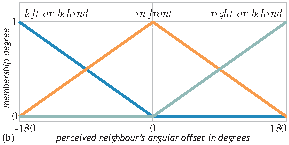
\includegraphics{fig_attraction_b}
  \par\vspace*{2mm}
  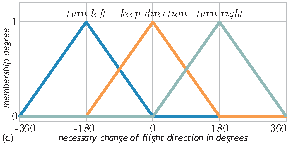
\includegraphics{fig_attraction_c}\hspace*{2mm}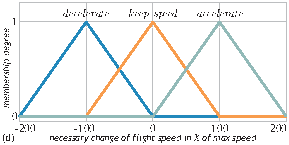
\includegraphics{fig_attraction_d}
  \par\vspace*{2mm}
  \caption{Membership functions of the fuzzy values `close enough', `too far' (a), `in front', `left or behind', `right or behind' (b), `turn left', `keep direction', `turn right' (c), `decelerate', `keep speed', `accelerate' (d) for the case of the attraction drive.}
  \label{fig:fuzzyAnimat:Da:afd}
\end{figure}
%
However, this is only one of the many possible interpretations of `close enough' and an interesting question is: when does a bird consider its neighbour to be `close enough'? Here comes into play the expertise of field ornithologists, who could use a tool such as this to translate their observational knowledge into simulation models.

In a similar fashion the fuzzy values `too far', `in front', `left or behind' and `right or behind' can be defined (\figs~\ref{fig:fuzzyAnimat:Da:afd}a and b). Furthermore, by introducing the fuzzy values `keep direction', `turn left', `turn right', `keep speed', `accelerate' and `decelerate' (\figs~\ref{fig:fuzzyAnimat:Da:afd}c and d) to represent the actions of keeping the same flight direction, performing a left turn and performing a right turn, keeping the same flight speed, accelerating and decelerating, the initial description can be rewritten in the form of a set of if-then rules denoted as the \emph{attraction fuzzy rule base}.

{\footnotesize
\begin{tabbing}
  \quad \= \frule{a1}: \quad \= \kwd{if} \=(\fvar{distance} \kwd{is} \fval{close enough}) \kwd{then} (\fvar{flight direction} \kwd{is} \fval{keep direction}), \\
  \> \frule{a2}: \> \kwd{if} (\fvar{distance} \kwd{is} \fval{too far}) \kwd{then} (\fvar{flight direction} \kwd{is} \fval{keep direction}), \\
  \> \frule{a3}: \> \kwd{if} (\fvar{distance} \kwd{is} \fval{close enough}) \kwd{then} (\fvar{flight speed} \kwd{is} \fval{keep speed}), \\
  \> \frule{a4}: \> \kwd{if} (\fvar{distance} \kwd{is} \fval{too far}) \kwd{then} (\fvar{flight speed} \kwd{is} \fval{keep speed}), \\
  \> \frule{a5}: \> \kwd{if} (\fvar{distance} \kwd{is} \fval{too far}) \kwd{and} (\fvar{position} \kwd{is} \fval{in front}) \kwd{then} (\fvar{flight speed} \kwd{is} \fval{accelerate}), \\
  \> \frule{a6}: \> \kwd{if} (\fvar{distance} \kwd{is} \fval{too far}) \kwd{and} (\fvar{position} \kwd{is} \fval{left or behind}) \kwd{then} (\fvar{flight direction} \kwd{is} \fval{turn left}), \\
  \> \frule{a7}: \> \kwd{if} (\fvar{distance} \kwd{is} \fval{too far}) \kwd{and} (\fvar{position} \kwd{is} \fvar{left or behind}) \kwd{then} (\fvar{flight speed} \kwd{is} \fval{decelerate}), \\
  \> \frule{a8}: \> \kwd{if} (\fvar{distance} \kwd{is} \fval{too far}) \kwd{and} (\fvar{position} \kwd{is} \fvar{right or behind}) \kwd{then} (\fvar{flight direction} \kwd{is} \fval{turn right}), \\
  \> \frule{a9}: \> \kwd{if} (\fvar{distance} \kwd{is} \fval{too far}) \kwd{and} (\fvar{position} \kwd{is} \fvar{right or behind}) \kwd{then} (\fvar{flight speed} \kwd{is} \fval{decelerate}).
\end{tabbing}
}

The first four rules from the attraction fuzzy rule base (\ie\ rules \frule{a1}--\frule{a4}) model the assumption that a bird in general tends not to change its flight direction or flight speed; item (1) in the description on page~\pageref{dscr:attraction}. Rules \frule{a2} and \frule{a4} model the assumption that a bird, in order to keep close to a neighbour that is already close enough, does not need to do anything; item (2). Rule \frule{a5} models the assumption that a bird, in order to catch up with a neighbour that is in front of it but too far, needs only to speed up; item (3). Finally, the last four rules (\frule{a6}--\frule{a9}) model the assumption that a bird, in order to get close to a neighbour that is too far but positioned sideways or behind, needs to turn toward it and slow down; items (4) and (5).

The attraction fuzzy rule base can be used to model the fuzzy animat's attraction drive. When the fuzzy animat perceives only one neighbour, its uncertain action (\ie\ the changes in flight direction and/or flight speed as fuzzy sets) is computed by applying fuzzy logic on each of the rules and combining the rule outputs. The resulting action will keep the animat close to the perceived neighbour. When the fuzzy animat perceives more than one neighbour the rules are evaluated for each neighbour independently (\ie\ as if the animat perceived only that neighbour) and all outputs are combined (see section~\ref{sec:fuzzyAnimat:decision}). The resulting action is a combination that will satisfy the fuzzy animat's drive to keep close to all of the perceived neighbours. In any case the resulting uncertain action is given through the fuzzy set representing the required uncertain change in flight direction and the fuzzy set representing the required uncertain change in flight speed.

Recall that my fuzzy animat uses only one fuzzy perception function (\ie\ the fuzzy visual perception function---definition~\ref{def:fuzzyAnimat:Pv:afd}). This means that the set representing uncertain information that can be obtained from the current perceivable state of the universe is $\fpowset{\set{P}}=\fpowset{\set{P}^\textnormal{v}}=\fpowset{\N_n} \times \fpowset{\set{I}^\textnormal{v}}^n$ and that $\set{I}^\textnormal{v}=\R^4$. Furthermore, recall that the perception is accurate, which means that the fuzzy neighbourhood $\langle \fset{N}, \fset{O} \rangle \in \fpowset{\set{P}}$ is crisp (\ie\ the fuzzy sets $\fset{N} \in \fpowset{\N_n}$ and $\fset{O} \in \fpowset{\set{I}^\textnormal{v}}^n$ represent crisp sets). This means that the uncertain information about fuzzy animat $\fautom{B}_i$ is actually represented by the quadruple $\langle \varepsilon_i, \varphi_i, \varsigma_i, \vartheta_i \rangle \in \fpowset{\set{I}^\textnormal{v}}$ (\ie\ the crisp distance, crisp angular offset, crisp difference in flight speed and crisp difference in flight direction between the observed fuzzy animat and fuzzy animat $\fautom{B}_i$). In addition it also means that the fuzzy set of indexes of the relevant fuzzy animats is a crisp set (\ie\ $\mu_\fset{N}(i) \in \left\{0,1\right\}$ for all $i \in \N_n$).

As discussed earlier, my fuzzy animat can act only by changing its flight direction and/or flight speed. In other words: the set representing all possible actions is $\set{A}=\R^2$. The uncertain action (\ie\ the required uncertain flight direction change given as the fuzzy set $\fset{D} \in \fpowset{\R}$ and the required uncertain flight speed change given as the fuzzy set $\fset{S} \in \fpowset{\R}$) that with respect to the perceived uncertain information about the state of the universe $\langle \fset{N}, \fset{O} \rangle \in \fpowset{\set{P}}$ and the current state of the fuzzy animat $q$ satisfy the attraction drive is therefore given as $\fset{A}_\textnormal{a}=\langle \fset{D}_\textnormal{a}, \fset{S}_\textnormal{a} \rangle \in \fpowset{\set{A}}$.

\begin{definition}
  \label{def:fuzzyAnimat:Da:afd}
  Let the fuzzy neighbourhood returned by the visual perception function be $\fset{P}_\textnormal{v}=\langle \fset{N}, \fset{O} \rangle \in \fpowset{\set{P}}$, where $\fset{N}$ is the fuzzy set of indexes of the relevant fuzzy animats and $\fset{O} \in \fpowset{\set{I}^\textnormal{v}}^n$ represents uncertain information about the existing fuzzy animats. The \emph{fuzzy attraction drive function} $\ffunc{D}_\textnormal{a}: \fpowset{\set{P}} \times \set{Q} \mapsto \fpowset{\set{A}}$ can therefore be written as
  \begin{equation}
    \ffunc{D}_\textnormal{a}(\fset{P}_\textnormal{v},q)=%\langle \fset{D}_\textnormal{a}, \fset{S}_\textnormal{a} \rangle =
     \biguplus_{\forall i(\mu_\fset{N}(i)=1)} \mathcal{L}_\texttt{a}(\langle \varepsilon_i, \varphi_i, \varsigma_i, \vartheta_i \rangle),
  \end{equation}
  where $\mathcal{L}_\texttt{a}: \fpowset{\set{I}^\textnormal{v}} \mapsto \fpowset{\set{A}}$ denotes the application of fuzzy logic on the attraction fuzzy rule base with $\fvar{distance}=\varepsilon_i$ and $\fvar{position}=\varphi_i$.
\end{definition}

%-
\subsubsection{The Fuzzy Repulsion Drive}
The primary motive of the repulsion drive is to stay away from collisions. I shall again assume that the hypothetical bird perceives only one neighbour, except that this time I am interested in the action that will keep it away from colliding with that neighbour. Using common sense, most of us would describe the bird's behaviour in the following way:
\begin{enumerate}
  \item in general do not change flight speed or flight direction;
  \item when the perceived neighbour is `far enough', change neither flight speed nor flight direction;
  \item when the perceived neighbour is `too close' and anywhere `behind', speed up;
  \item when the perceived neighbour is `too close' and `in front or right', turn away from it and slow down;
  \item when the perceived neighbour is `too close' and `in front or left', turn away from it and slow down.
\end{enumerate}

Once more it can be noticed that in the description the resulting action depends only on the perceived neighbour's distance and position. Therefore, as in the case of the attraction drive, I shall first define the fuzzy values `far enough', `too close', `behind', `in front or right' and `in front or left' (\figs~\ref{fig:fuzzyAnimat:Dr:afd}a and b).
%
\begin{figure}
  \null\vspace*{2mm}\par
  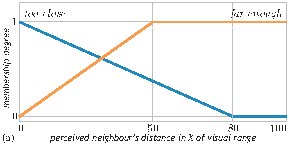
\includegraphics{fig_repulsion_a}\hspace*{2mm}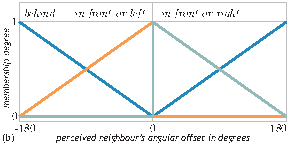
\includegraphics{fig_repulsion_b}
  \par\vspace*{2mm}
  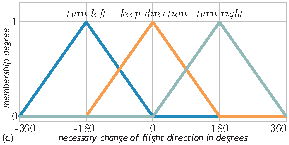
\includegraphics{fig_repulsion_c}\hspace*{2mm}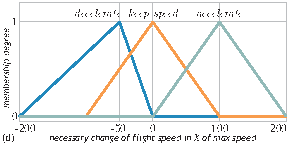
\includegraphics{fig_repulsion_d}
  \par\vspace*{2mm}
  \caption{Membership functions of the fuzzy values `too close', `far enough' (a), `behind', `in front or left', `in front or right' (b), `turn left', `keep direction', `turn right' (c), `decelerate', `keep speed', `accelerate' (d) for the case of the repulsion drive.}
  \label{fig:fuzzyAnimat:Dr:afd}
\end{figure}
%
Then, assuming that the bird can act only by changing its flight direction and/or flight speed, I shall introduce the fuzzy values that represent the actions of keeping the same flight direction, performing a left turn, \etc\ (\figs~\ref{fig:fuzzyAnimat:Dr:afd}c and d). After completing these two steps the initial description can be rewritten in the form of a set of if-then rules that I shall denote as the \emph{repulsion fuzzy rule base}.

{\footnotesize
\begin{tabbing}
  \quad \= \frule{r1}: \quad \= \kwd{if} \=(\fvar{distance} \kwd{is} \fval{far enough}) \kwd{then} (\fvar{flight direction} \kwd{is} \fval{keep direction}), \\
  \> \frule{r2}: \> \kwd{if} (\fvar{distance} \kwd{is} \fval{too close}) \kwd{then} (\fvar{flight direction} \kwd{is} \fval{keep direction}), \\
  \> \frule{r3}: \> \kwd{if} (\fvar{distance} \kwd{is} \fval{far enough}) \kwd{then} (\fvar{flight speed} \kwd{is} \fval{keep speed}), \\
  \> \frule{r4}: \> \kwd{if} (\fvar{distance} \kwd{is} \fval{too close}) \kwd{then} (\fvar{flight speed} \kwd{is} \fval{keep speed}), \\
  \> \frule{r5}: \> \kwd{if} (\fvar{distance} \kwd{is} \fval{too close}) \kwd{and} (\fvar{position} \kwd{is} \fval{behind}) \kwd{then} (\fvar{flight speed} \kwd{is} \fval{accelerate}), \\
  \> \frule{r6}: \> \kwd{if} (\fvar{distance} \kwd{is} \fval{too close}) \kwd{and} (\fvar{position} \kwd{is} \fval{in front or left}) \kwd{then} (\fvar{flight direction} \kwd{is} \fval{turn right}), \\
  \> \frule{r7}: \> \kwd{if} (\fvar{distance} \kwd{is} \fval{too close}) \kwd{and} (\fvar{position} \kwd{is} \fvar{in front or left}) \kwd{then} (\fvar{flight speed} \kwd{is} \fval{decelerate}), \\
  \> \frule{r8}: \> \kwd{if} (\fvar{distance} \kwd{is} \fval{too close}) \kwd{and} (\fvar{position} \kwd{is} \fvar{in front or right}) \kwd{then} (\fvar{flight direction} \kwd{is} \fval{turn left}), \\
  \> \frule{r9}: \> \kwd{if} (\fvar{distance} \kwd{is} \fval{too close}) \kwd{and} (\fvar{position} \kwd{is} \fvar{in front or right}) \kwd{then} (\fvar{flight speed} \kwd{is} \fval{decelerate}).
\end{tabbing}
}

As in the case of the attraction drive, the repulsion fuzzy rule base can be used to model the fuzzy animat's repulsion drive. In other words, for each of the perceived neighbours the fuzzy animat applies fuzzy logic on each of the rules from the repulsion fuzzy rule base and works out the uncertain action that should be taken to keep away from colliding with any of the perceived neighbours (see section~\ref{sec:fuzzyAnimat:decision}).

\begin{definition}
  \label{def:fuzzyAnimat:Dr:afd}
  Let the fuzzy neighbourhood returned by the visual perception function be $\fset{P}_\textnormal{v}=\langle \fset{N}, \fset{O} \rangle \in \fpowset{\set{P}}$, where $\fset{N}$ is the fuzzy set of indexes of the relevant fuzzy animats and $\fset{O} \in \fpowset{\set{I}^\textnormal{v}}^n$ represents uncertain information about the existing fuzzy animats. The \emph{fuzzy repulsion drive function} $\ffunc{D}_\textnormal{r}:\fpowset{\set{P}} \times \set{Q} \mapsto \fpowset{\set{A}}$ can therefore be written as
  \begin{equation}
  \ffunc{D}_\textnormal{r}(\fset{P}_\textnormal{v},q)=%\langle \fset{D}_\textnormal{r}, \fset{S}_\textnormal{r} \rangle =
   \biguplus_{\forall i(\mu_\fset{N}(i)=1)} \mathcal{L}_\texttt{r}(\langle \varepsilon_i, \varphi_i, \varsigma_i, \vartheta_i \rangle),
  \end{equation}
  where $\mathcal{L}_\texttt{r}: \fpowset{\set{I}^\textnormal{v}} \mapsto \fpowset{\set{A}}$ denotes the application of fuzzy logic on the repulsion fuzzy rule base with $\fvar{distance}=\varepsilon_i$ and $\fvar{position}=\varphi_i$.
\end{definition}

%-
\subsubsection{The Fuzzy Alignment Drive}
The alignment drive's motive is to achieve polarization with flockmates (\ie\ to keep approximately the same flight speed and flight direction as the perceived flockmates). If it is yet again assumed that the hypothetical bird perceives only one neighbour then the necessary actions can be described as follows:

\begin{enumerate}
  \item in general do not change flight speed or flight direction;
  \item when the perceived neighbour is `too far' or `too close', change neither flight speed nor flight direction;
  \item when the perceived neighbour is at a `good' distance and flying in the `same direction', keep flight direction;
  \item when the perceived neighbour is at a `good' distance but flying more to the `left', turn left;
  \item when the perceived neighbour is at a `good' distance but flying more to the `right', turn right;
  \item when the perceived neighbour is at a `good' distance and flying with the `same speed', keep flight speed;
  \item when the perceived neighbour is at a `good' distance but flying `slower', slow down;
  \item when the perceived neighbour is at a `good' distance but flying `faster', speed up.
\end{enumerate}

\begin{figure}
  \null\vspace*{2mm}\par
  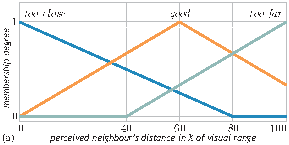
\includegraphics{fig_alignment_a}\hspace*{2mm}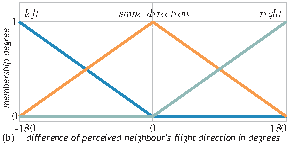
\includegraphics{fig_alignment_b}
  \par\vspace*{2mm}
  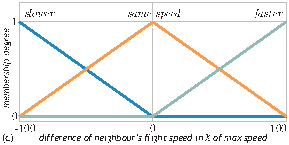
\includegraphics{fig_alignment_c}
  \par\vspace*{2mm}
  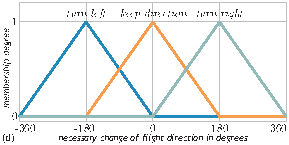
\includegraphics{fig_alignment_d}\hspace*{2mm}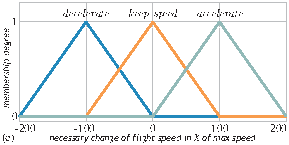
\includegraphics{fig_alignment_e}
  \par\vspace*{2mm}
  \caption{Membership functions of the fuzzy values `too close', `good', `too far' (a), `left', `same direction', `right' (b), `slower', `same speed', `faster' (c), `turn left', `keep direction', `turn right' (d), `decelerate', `keep speed', `accelerate' (e) for the case of the alignment drive.}
  \label{fig:fuzzyAnimat:Dp:afd}
\end{figure}

As a contrast to the attraction and repulsion drives it can be noticed that in this case the action depends on the perceived neighbour's distance, difference in flight direction and difference in flight speed. After the definition and introduction of the required fuzzy values (\fig~\ref{fig:fuzzyAnimat:Dp:afd}) the initial description can be rewritten in the form of the \emph{alignment fuzzy rule base}.

{\footnotesize
\begin{tabbing}
  \quad \= \frule{p1}: \quad \= \kwd{if} \=(\fvar{distance} \kwd{is} \fval{too far}) \kwd{then} (\fvar{flight direction} \kwd{is} \fval{keep direction}), \\
  \> \frule{p2}: \> \kwd{if} (\fvar{distance} \kwd{is} \fval{too close}) \kwd{then} (\fvar{flight direction} \kwd{is} \fval{keep direction}), \\
  \> \frule{p3}: \> \kwd{if} (\fvar{distance} \kwd{is} \fval{too far}) \kwd{then} (\fvar{flight speed} \kwd{is} \fval{keep speed}), \\
  \> \frule{p4}: \> \kwd{if} (\fvar{distance} \kwd{is} \fval{too close}) \kwd{then} (\fvar{flight speed} \kwd{is} \fval{keep speed}), \\
  \> \frule{p5}: \> \kwd{if} (\fvar{distance} \kwd{is} \fval{good}) \kwd{and} (\fvar{direction} \kwd{is} \fval{same direction}) \kwd{then} (\fvar{flight direction} \kwd{is} \fval{keep direction}), \\
  \> \frule{p6}: \> \kwd{if} (\fvar{distance} \kwd{is} \fval{good}) \kwd{and} (\fvar{direction} \kwd{is} \fval{left}) \kwd{then} (\fvar{flight direction} \kwd{is} \fval{turn left}), \\
  \> \frule{p7}: \> \kwd{if} (\fvar{distance} \kwd{is} \fval{good}) \kwd{and} (\fvar{direction} \kwd{is} \fval{right}) \kwd{then} (\fvar{flight direction} \kwd{is} \fval{turn right}), \\
  \> \frule{p8}: \> \kwd{if} (\fvar{distance} \kwd{is} \fval{good}) \kwd{and} (\fvar{speed} \kwd{is} \fval{same speed}) \kwd{then} (\fvar{flight speed} \kwd{is} \fval{keep speed}), \\
  \> \frule{p9}: \> \kwd{if} (\fvar{distance} \kwd{is} \fval{good}) \kwd{and} (\fvar{speed} \kwd{is} \fvar{slower}) \kwd{then} (\fvar{flight speed} \kwd{is} \fval{decelerate}), \\
  \> \frule{p10}: \> \kwd{if} (\fvar{distance} \kwd{is} \fval{good}) \kwd{and} (\fvar{speed} \kwd{is} \fvar{faster}) \kwd{then} (\fvar{flight speed} \kwd{is} \fval{accelerate}).
\end{tabbing}
}

Yet again the alignment fuzzy rule base can be used to model the fuzzy animat's alignment drive. That is, by applying fuzzy logic on it, the fuzzy animat can work out the uncertain action that should be taken in order to keep approximately the same flight speed and flight direction as the perceived neighbours (see section~\ref{sec:fuzzyAnimat:decision}).

\begin{definition}
  \label{def:fuzzyAnimat:Dp:afd}
  Let the fuzzy neighbourhood returned by the visual perception function be $\fset{P}_\textnormal{v}=\langle \fset{N}, \fset{O} \rangle \in \fpowset{\set{P}}$, where $\fset{N}$ is the fuzzy set of indexes of the relevant fuzzy animats and $\fset{O} \in \fpowset{\set{I}^\textnormal{v}}^n$ represents uncertain information about the existing fuzzy animats. The \emph{fuzzy alignment drive function} $\ffunc{D}_\textnormal{p}: \fpowset{\set{P}} \times \fset{Q} \mapsto \fpowset{\set{A}}$ can therefore be written as
  \begin{equation}
    \ffunc{D}_\textnormal{p}(\fset{P}_\textnormal{v},q)=%\langle \fset{D}_\textnormal{p}, \fset{S}_\textnormal{p} \rangle =
     \biguplus_{\forall i(\mu_\fset{N}(i)=1)} \mathcal{L}_\texttt{p}(\langle \varepsilon_i, \varphi_i, \varsigma_i, \vartheta_i \rangle),
  \end{equation}
  where $\mathcal{L}_\texttt{p}: \fpowset{\set{I}^\textnormal{v}} \mapsto \fpowset{\set{A}}$ denotes the application of fuzzy logic on the alignment fuzzy rule base, where $\fvar{distance}=\varepsilon_i$, $\fvar{speed}=\varsigma_i$ and $\fvar{direction}=\vartheta_i$.
\end{definition}

%--
\subsection{Modelling Action Selection}
As already discussed, the action selection process simulates the animal's neurological process of selecting the sequence of muscular movements that will accomplish the actions that result from its drives. This process combines, prioritizes, and arbitrates between potentially conflicting actions. Similar to Reynolds \cite{reynolds:1987,reynolds:1999} (subsection~\ref{subsec:animat:cwr}) and Heppner and Grenander \cite{heppner:1990} (subsection~\ref{subsec:animat:fhh}), in my study I do not model the musculoskeletal structure of a real bird and model the action selection mechanism as a simple combination of the actions that result from the animat's drives. In other words, for each of the animat's drives a vector is calculated that represents the force needed to accomplish the required action. These forces are then combined by using a weighted sum and the resulting vector used to calculate the animat's new flight speed and flight direction. This calculation is subjected to a set of constraints modelling conservation of momentum, viscous damping and the animal's finite amount of available energy. The same approach named geometrical flight was already used by Reynolds \cite{reynolds:1987,reynolds:1999} (see subsection~\ref{subsec:animat:cwr}). Heppner and Grenander \cite{heppner:1990}, who represented actions as vectors (see subsection~\ref{subsec:animat:fhh}), used a similar approach and modelled action selection as a simple weighted sum. However, apart from the Poisson stochastic process modelling the effects of wind gusts and random local disturbances, they did not apply any additional constraints.

To sum up, my fuzzy animat is based on a point mass approximation. The same approach, named a point mass vehicle model, was used by Reynolds \cite{reynolds:1987,reynolds:1999} (see subsection~\ref{subsec:animat:cwr}). This means that my fuzzy animat's physics is also based on forward Euler integration \cite{parent:2002,reynolds:1999}. As said, for each of the fuzzy animat's three fuzzy drives (\ie\ the fuzzy attraction, fuzzy repulsion and fuzzy alignment drive) a vector is calculated that represents the force needed to accomplish the required action. However, in my case, the uncertain action resulting from a fuzzy drive gives the required uncertain change in flight direction and the required uncertain change in flight speed as fuzzy sets. This means that each of the two fuzzy sets needs first to be converted into a single (crisp) value which, in some sense, is the best representative of the fuzzy set. This is achieved through defuzzification (see subsection~\ref{subsec:fuzzyModelling:fuzzyRuleBase}). The defuzzified values are then used to compute the forces required to initiate the desired changes and these are afterwards combined by using a weighted sum. \sidenote{The weights have been chosen so as to give the highest priority to the fuzzy repulsion drive, followed by the fuzzy alignment drive, and the lowest priority to the fuzzy attraction drive.}{v1.0.20050124 [MM]: provide an explanation why so.\\v1.3.20050407 [BZ]: Why? Any analysis on what would changes cause?\\v1.4.20050412 [ILB]: This was based both on the weights employed by Reynolds and on the analysis of the importance of the separation, alignment and cohesion drive used in his model \cite{lebar_bajec:2002,lebar_bajec:2003a}.} The resulting vector is used to calculate the fuzzy animat's new flight speed and flight direction. In other words, the resulting force (limited by the fuzzy animat's available force) is applied to the fuzzy animat's point mass. This produces an acceleration equal to the force divided by the fuzzy animat's mass. The acceleration is then added to the fuzzy animat's current velocity vector and truncated by the maximum achievable speed. Finally the fuzzy animat's new position is computed by adding the new velocity vector to the fuzzy animat's current position.

Let $\vect{a} \in \E$ be a vector. Then since I am using the two-dimensional Euclidean vector space $\E=\R^2$ the rotation of vector $\vect{a}$ for the angle $\alpha$ is defined as
%
\begin{equation}
  R(\vect{a}, \alpha) = \left(\vect{a}_\textnormal{x}\cos\alpha + \vect{a}_\textnormal{y}\sin\alpha\right)\vect{e}_\textnormal{i} + \left(-\vect{a}_\textnormal{x}\sin\alpha + \vect{a}_\textnormal{y}\cos\alpha\right)\vect{e}_\textnormal{j},
\end{equation}
%
where $\vect{e}_\textnormal{i}$, $\vect{e}_\textnormal{j}$ are the $\mathrm{x}$ and $\mathrm{y}$ axis unit vectors of the Cartesian coordinate system.

Furthermore, if $a \in \R^+$ is used to represent the maximal size of vector $\vect{a}$, equation~\eqref{eq:truncation} still holds, and truncation of vector $\vect{a}$ so that its size is lower or equal $a$ is computed as
%
\begin{equation}
  \lfloor\vect{a}\rceil^{a} = \min(\left\|\vect{a}\right\|, a) \vect{a}^0. \nonumber
\end{equation}

Let $\fset{A}=\langle \fset{D}, \fset{S} \rangle \in \fpowset{\set{A}}$ represent the desired uncertain action returned by one of the fuzzy drive functions from definitions~\ref{def:fuzzyAnimat:Da:afd}--\ref{def:fuzzyAnimat:Dp:afd}. Let the fuzzy set $\fset{D}$ represent the desired uncertain flight direction change and let the fuzzy set $\fset{S}$ the desired uncertain flight speed change. Let the current state of the observed fuzzy animat be $q=\langle \vect{p}, \vect{v}, s \rangle$, where $\vect{p}$ is the fuzzy animat's current position in space, $\vect{v}$ its velocity and $s$ the modelled animal's internal state defined by definition~\ref{def:fuzzyAnimat:s:afd}. Then the mapping $F: \fpowset{\set{A}} \times \set{Q} \mapsto \E$ given by equation~\eqref{eq:fuzzyAnimat:Sws:force:afd} computes the force required to initiate the desired change in flight speed and/or flight direction.
\begin{equation}
  F(\fset{A},q)=\left\lfloor\max(\left\|\vect{v}\right\|+\cog\fset{S},0)R(\vect{v}^0,\cog\fset{D})\right\rceil^{v_\textnormal{M}}-\vect{v}. \label{eq:fuzzyAnimat:Sws:force:afd}
\end{equation}

\begin{definition}
  \label{def:fuzzyAnimat:Sws:afd}
  Let the current state of the fuzzy animat be $q=\langle\vect{p},\vect{v},s\rangle$, where the modelled animal's internal state $s$ is defined by definition~\ref{def:fuzzyAnimat:s:afd}. Let the computed desired uncertain actions be $\langle \fset{A}_\textnormal{a},\fset{A}_\textnormal{r},\fset{A}_\textnormal{p}\rangle$. Let $w_\textnormal{a}$, $w_\textnormal{r}$ and $w_\textnormal{p}$ represent the weight of the fuzzy attraction, fuzzy repulsion and fuzzy alignment drive respectively and let $dt$ represent the simulation step. Then the \emph{fuzzy weighted sum action selection function} $\ffunc{S}_\textnormal{ws}: \fpowset{\set{A}} \times \set{Q} \mapsto \set{Q}$ is defined as
  \begin{equation}
    S_\textnormal{ws}(\langle \fset{A}_\textnormal{a},\fset{A}_\textnormal{r},\fset{A}_\textnormal{p}\rangle, q) = \langle\vect{p}', \vect{v}', s\rangle, \label{eq:fuzzyAnimat:Sws0:afd}
  \end{equation}
  \begin{equation}
    \vect{v}' = \left\lfloor {\vect{v} + \frac{\left\lfloor w_\textnormal{a}F(\fset{A}_\textnormal{a},q) + w_\textnormal{r}F(\fset{A}_\textnormal{r},q) + w_\textnormal{p}F(\fset{A}_\textnormal{p},q) \right\rceil^{f_\textnormal{M}}}{m}}dt \right\rceil^{v_\textnormal{M}},
  \end{equation}
  \begin{equation}
    \vect{p}' = \vect{p} + \vect{v}'dt. \label{eq:fuzzyAnimat:Sws2:afd}
  \end{equation}
\end{definition}

%--
\subsection{A Wingbeat of the Fuzzy Digital Bird}
\label{sec:fuzzyAnimat:decision}
In the previous sections a formal definition of a fuzzy digital bird was presented. With a collection of the latter, a fuzzy model for a computer simulation of bird flocking can be constructed. This section provides an example of the steps taken in processing a single decision. The main emphasis is given to the computation of the fuzzy drives.

Let the current state of the digital universe be such that the observed fuzzy animat perceives only two neighbours. Let neighbour $\fautom{B}_1$ be 80\% of the observed fuzzy animat's visual range away with an angular offset of \ang{-30} and neighbour $\fautom{B}_2$ 60\% of the visual range away with an angular offset of \ang{-110} (\fig~\ref{fig:attraction:FLS:ini}). For reasons of simplicity I shall assume that they are all flying in the same direction and with the same flight speed.

\begin{figure}
  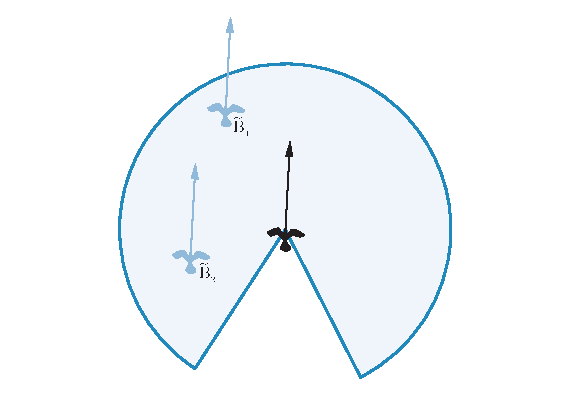
\includegraphics{fig_attractionFLSini}
  \caption{The observed fuzzy animat perceives two neighbours, one of which is 80\% of the visual range away with an angular offset of \ang{-30} ($\fautom{B}_1$), and the other is 60\% of the visual range away with an angular offset of \ang{-110} ($\fautom{B}_2$). All fuzzy animats have the same flight direction and flight speed (black and blue arrows).}
  \label{fig:attraction:FLS:ini}
\end{figure}

By computing the fuzzy attraction, fuzzy repulsion and fuzzy alignment drive (\ie\ applying fuzzy logic on the attraction, repulsion and alignment fuzzy rule bases) the observed fuzzy animat computes three independent actions (\ie\ uncertain flight direction and/or flight speed changes). These actions together will satisfy its drives to stay close to the perceived neighbours, keep away from colliding with them and fly in approximately the same direction and flight speed. With the fuzzy weighted sum action selection function the fuzzy animat then combines, prioritizes and arbitrates these actions and computes the flight direction and/or flight speed change to be taken in the following time step.

Even though all fuzzy drives can be computed simultaneously, let me start with the fuzzy attraction drive. For each of the perceived neighbours the fuzzy rule base is evaluated independently (\ie\ as if the fuzzy animat perceived only one neighbour) and all outputs are later combined. Now, recall that the action that satisfies the fuzzy attraction drive depends only on the perceived neighbour's distance and position. Because all of the perceived information is precise, for neighbour $\fautom{B}_1$, \fvar{distance} is the crisp value 80\% of the visual range and \fvar{position} is the crisp value \ang{-30}.

First let me compute the necessary change in flight direction (\ie\ evaluate rules \frule{a1}, \frule{a2}, \frule{a6} and \frule{a8} from the attraction fuzzy rule base). It is easy to notice that rules \frule{a1} and \frule{a2} have the same consequent (\ie\ `\fvar{distance} \kwd{is} \fval{keep direction}'). Because of this their antecedents can be joined, using the logical operator `\kwd{or}', and interpreted as a single rule. To assess the degree of truth of the compound antecedent the degrees of truth of the individual antecedents must first be computed and then the fuzzy logic operator `\kwd{or}' must be applied.

Let $\statement{A}_1$ denote the antecedent of rule \frule{a1} (\ie\ `\fvar{distance} \kwd{is} \fval{close enough}') and $\statement{A}_2$ the antecedent of rule \frule{a2} (\ie\ `\fvar{distance} \kwd{is} \fval{too far}'). Recall that as distance is a crisp value, the degrees of truth of $\statement{A}_1$ and $\statement{A}_2$ are given by the degree of membership of distance in the corresponding fuzzy sets (see subsection~\ref{subsec:fuzzyModelling:fuzzyLogic}). Therefore, if $d$ is used to denote the value of distance, $\fset{C}$ to denote the fuzzy set `close enough' and $\fset{F}$ the fuzzy set `too far', then
%
\begin{equation}
  \begin{array}{ll}
  T(\statement{A}_1)=\mu_\fset{C}(d)=\mu_\fset{C}(80)=0.33, \\
  T(\statement{A}_2)=\mu_\fset{F}(d)=\mu_\fset{F}(80)=0.67.
  \end{array}
\end{equation}
%
Since in this dissertation the logical operator `\kwd{or}' is interpreted as maximum fuzzy union, the degree of truth of the compound antecedent is
%
\begin{equation}
  T(\statement{A}_1\ \kwd{or}\ \statement{A}_2)=\max(T(\statement{A}_1),T(\statement{A}_2))=\max(0.33,0.67)=0.67.
\end{equation}
%
Recall that the degree of truth of the antecedent implies the degree of truth of the conclusion, and that fuzzy implication modifies the output fuzzy set (see subsection~\ref{subsec:fuzzyModelling:ifthen}). Let $\mu_\fset{K}$ denote the fuzzy set `keep direction'. Then, as this dissertation makes use of product fuzzy implication, which modifies the output fuzzy set by squashing it, the membership function of the modified output fuzzy set that results from rules \frule{a1} and \frule{a2} is given by
%
\begin{equation}
  \mu_{\fset{K}'}(r)=T(\statement{A}_1\ \kwd{or}\ \statement{A}_2) \cdot \mu_\fset{K}(r)=0.67 \cdot \mu_\fset{K}(r).
\end{equation}

\begin{figure}
  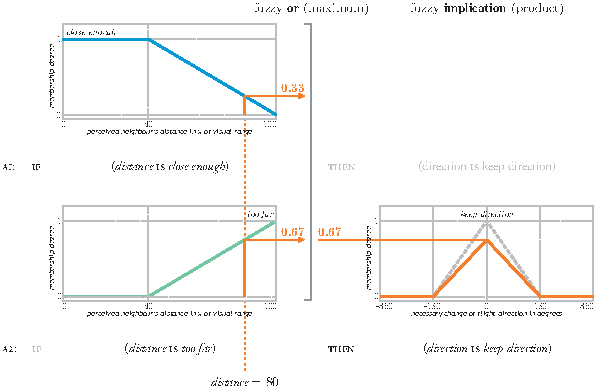
\includegraphics{fig_attractionFLSa1+a2}
  \caption{Graphical representation of the evaluation of rules \frule{a1} and \frule{a2} for the case when the perceived neighbour is 80\% of the visual range away with an angular offset of \ang{-30}. The left half shows the evaluation of the degrees of truth of the antecedents and the right part the modification of the output fuzzy set.}
  \label{fig:attraction:FLS:a1+a2}
\end{figure}

A graphical representation of the above described evaluation process is presented in figure~\ref{fig:attraction:FLS:a1+a2}. The left half shows the evaluation of the antecedents' degrees of truth, while the right shows the modification of the output fuzzy set.

Rules \frule{a6} and \frule{a8} have different consequents, which means that they, even though they can be evaluated simultaneously, cannot be treated as a single rule. It can be noticed, however, that their antecedents have multiple parts. In both cases the antecedent is composed of two conditions joined by the logical operator `\kwd{and}'. This means that to evaluate the degree of truth of the antecedent the degrees of truth of the individual conditions must first be computed and then the fuzzy logic operator `\kwd{and}' must be applied. A graphical representation of the evaluation process is presented in figure~\ref{fig:attraction:FLS:a6+a8}.

\begin{figure}
  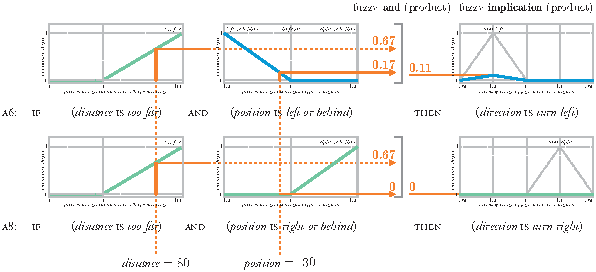
\includegraphics{fig_attractionFLSa6+a8}
  \caption{Graphical representation of the evaluation of rules \frule{a6} and \frule{a8} for the case when the perceived neighbour is 80\% of the visual range away with an angular offset of \ang{-30}. The left half shows the evaluation of the degrees of truth of the antecedents and the right part the modification of the output fuzzy sets.}
  \label{fig:attraction:FLS:a6+a8}
\end{figure}

For rule \frule{a6} let $\statement{A}_{61}$ denote condition `\fvar{distance} \kwd{is} \fval{too far}' and $\statement{A}_{62}$ condition `\fvar{position} \kwd{is} \fval{left or behind}'. Then, if $d$ is used to denote the value of distance, $p$ to denote the value of position, $\fset{F}$ the fuzzy set `too far' and $\fset{L}$ the fuzzy set `left or behind'
%
\begin{equation}
  \begin{array}{ll}
  T(\statement{A}_{61})=\mu_\fset{F}(d)=\mu_\fset{F}(80)=0.67, \\
  T(\statement{A}_{62})=\mu_\fset{L}(p)=\mu_\fset{L}(-30)=0.17,
  \end{array}
\end{equation}
%
and, because this dissertation uses product fuzzy intersection to interpret the logical operator `\kwd{and}', the degree of truth of the antecedent of rule \frule{a6} is
%
\begin{equation}
  T(\statement{A}_{61}\ \kwd{and}\ \statement{A}_{62})=T(\statement{A}_{61}) \cdot T(\statement{A}_{62})=0.67 \cdot 0.17 = 0.11.
\end{equation}
%
This means that, if $\fset{T}_\textnormal{L}$ is used to denote the fuzzy set `turn left', the membership function of the modified output fuzzy set that results from rule \frule{a6} is
%
\begin{equation}
  \mu_{{\fset{T}_\textnormal{L}}'}(r)=T(\statement{A}_{61}\ \kwd{and}\ \statement{A}_{62}) \cdot \mu_{\fset{T}_\textnormal{L}}(r)=0.11 \cdot \mu_{\fset{T}_\textnormal{L}}(r).
\end{equation}

Similarly for rule \frule{a8} condition `\fvar{distance} \kwd{is} \fval{too far}' is denoted as $\statement{A}_{81}$ and condition `\fvar{position} \kwd{is} \fval{right or behind}' as $\statement{A}_{82}$. Then, if the fuzzy set `right or behind' is denoted as $\fset{R}$, it can be written that
%
\begin{equation}
  \begin{array}{ll}
  T(\statement{A}_{81})=\mu_\fset{F}(d)=\mu_\fset{F}(80)=0.67, \\
  T(\statement{A}_{82})=\mu_\fset{R}(p)=\mu_\fset{R}(-30)=0,
  \end{array}
\end{equation}
%
and the degree of truth of the antecedent of rule \frule{a8} is
%
\begin{equation}
  T(\statement{A}_{81}\ \kwd{and}\ \statement{A}_{82})=T(\statement{A}_{81}) \cdot T(\statement{A}_{82})=0.67 \cdot 0 = 0,
\end{equation}
%
which means that the antecedent is false.

For neighbour $\fautom{B}_2$ the membership function of the modified output fuzzy set that results from rules \frule{a1} and \frule{a2} is given by
%
\begin{equation}
  \begin{array}{rl}
  \mu_{\fset{K}'}(r)&=T(\statement{A}_1\ \kwd{or}\ \statement{A}_2) \cdot \mu_\fset{K}(r)=\max(\mu_\fset{C}(60),\mu_\fset{F}(60)) \cdot \mu_\fset{K}(r)= \\
                    &=\max(0.67,0.33) \cdot \mu_\fset{K}(r)=0.67 \cdot \mu_\fset{K}(r),
  \end{array}
\end{equation}
%
the modified output fuzzy set that results from rule \frule{a6} by
%
\begin{equation}
  \begin{array}{rl}
  \mu_{{\fset{T}_\textnormal{L}}'}(r)&=T(\statement{A}_{61}\ \kwd{and}\ \statement{A}_{62}) \cdot \mu_{\fset{T}_\textnormal{L}}(r)=\\
                                 &=\left(\mu_\fset{F}(60) \cdot \mu_\fset{L}(-110)\right) \cdot \mu_{\fset{T}_\textnormal{L}}(r)=\\
                                 &=\left(0.33 \cdot 0.61\right) \cdot \mu_{\fset{T}_\textnormal{L}}(r)=0.2 \cdot \mu_{\fset{T}_\textnormal{L}}(r),
  \end{array}
\end{equation}
%
whereas the antecedent of rule \frule{a8} is again false.

Rules whose antecedents are true to a non-zero degree are usually denoted as \emph{active} rules. In my case the modified output fuzzy set that results from the consequent of an active rule represents the uncertain flight direction change according to that rule, expressed in the form of a fuzzy set. But because in fuzzy logic more than one rule can be active at a time and because the rules are evaluated for each perceived neighbour individually, all of the modified output fuzzy sets have to be combined into a single fuzzy set (see subsection~\ref{subsec:fuzzyModelling:fuzzyRuleBase}). This is done by computing the fuzzy union of the modified output fuzzy sets. This dissertation makes use of the algebraic sum fuzzy union (see \chaptername~\ref{ch:fuzzyModelling}). The combined fuzzy set that was obtained by evaluating the fuzzy rule base for the two perceived neighbours is presented in figure~\ref{fig:attraction:FLS:combined}.

\begin{figure}
  \null\vspace*{2mm}
  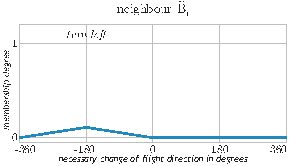
\includegraphics{fig_attractionFLScombined_a}\hspace*{2mm}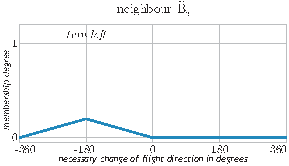
\includegraphics{fig_attractionFLScombined_b}
  \par\vspace*{2mm}
  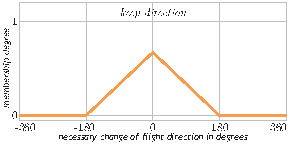
\includegraphics{fig_attractionFLScombined_c}\hspace*{2mm}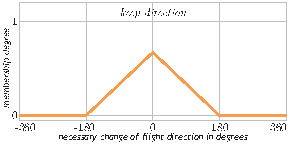
\includegraphics{fig_attractionFLScombined_d}
  \par\vspace*{2mm}
  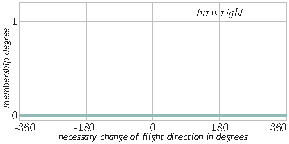
\includegraphics{fig_attractionFLScombined_e}\hspace*{2mm}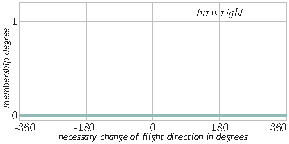
\includegraphics{fig_attractionFLScombined_f}
  \par\vspace*{2mm}
  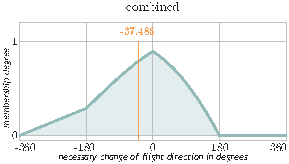
\includegraphics{fig_attractionFLScombined_g}
  \par\vspace*{2mm}
  \caption{The modified output fuzzy sets that result from active rules and represent the flight direction change candidates. They were obtained by evaluating the attraction drive fuzzy rule base for the case when the only two perceived neighbours are 80\% of the visual range away with an angular offset of \ang{-30} ($\fautom{B}_1$), and 60\% of the visual range away with an angular offset of \ang{-110} ($\fautom{B}_2$). The combined fuzzy set is the algebraic sum fuzzy union of the modified output fuzzy sets. The defuzzified value, obtained by using the centroid method, equals \ang{-37.485}.}
  \label{fig:attraction:FLS:combined}
\end{figure}

Even though the combined fuzzy set represents the flight direction change that will help satisfy the attraction drive it is still a fuzzy set. Therefore, in the final step, it has to be converted into a single (crisp) value that is, in some sense, the best representative of the fuzzy set. This is achieved through defuzzification. In this dissertation the centroid defuzzification method is used, which  returns the single (crisp) value, for which the area under the graph of the membership function of the combined fuzzy set is divided into two equal subareas (see subsection~\ref{subsec:fuzzyModelling:fuzzyRuleBase}).

If I return to the example: the defuzzified value resulting from the combined fuzzy set presented in figure~\ref{fig:attraction:FLS:combined} is \ang{-37.485}. This means that in order to satisfy the fuzzy attraction drive, the fuzzy animat should turn to the left by \ang{37.485}. By computing the necessary change in flight speed it can be found out that the fuzzy animat, in order to satisfy the fuzzy attraction drive, should also increase its flight speed by 17.3489\% of its maximal achievable flight speed.\footnote{It is important to note that if the fuzzy animat is already flying at its maximal achievable flight speed, it will keep on flying at this speed and the desired increase will remain unaccomplished. This will happen due to the truncation of the flight speed in the fuzzy weighted sum action selection function.} The fuzzy repulsion drive would be satisfied with a turn to the right by \ang{11.078} and a speed increase of 4.3825\% of its maximal achievable flight speed. Since the fuzzy animat and the perceived neighbours have the same flight direction and flight speed, the fuzzy alignment drive does not require any changes (\fig~\ref{fig:attraction:FLS:output}).

\begin{figure}
  \null\vspace*{.5\gridH}
  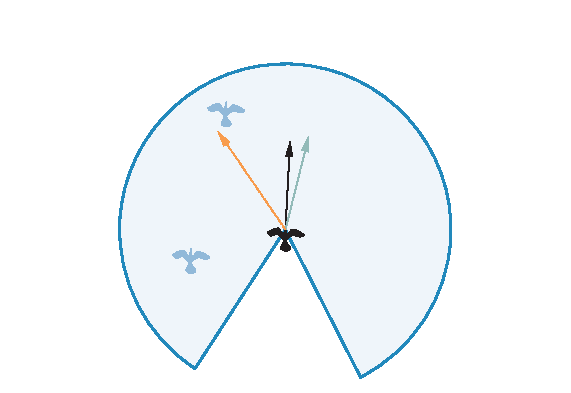
\includegraphics{fig_attractionFLSout}
  \vspace*{.5\gridH}
  \caption{The defuzzified desired flight direction and flight speed changes in the case when the observed fuzzy animat perceives only two neighbours. One neighbour is 80\% of the visual range away with an angular offset of \ang{-30}, and the other 60\% of the visual range away with an angular offset of \ang{-110}. All have the same flight direction and flight speed. The orange arrow represents the flight direction and flight speed change that would satisfy the fuzzy attraction drive, while the green arrow represents the flight direction and speed change that would satisfy the fuzzy repulsion drive.}
  \label{fig:attraction:FLS:output}
\end{figure}

 	% !TeX root = ./thesis.tex










%==============================
\chapter{Behaviour Analysis}
\label{ch:analysis}


%----
\section{Metrics}
\label{sec:analysis:metrics}
In \chaptername~\ref{ch:animat} the formal definition of the animat was presented. Its potential as a construction framework for modelling the dynamics of organized groups of moving animals was shown, by using it to reproduce Reynold's \cite{reynolds:1987,reynolds:1999} and Heppner and Grenander's \cite{heppner:1990} computer model of bird flocking. By introducing fuzziness into the animat in \chaptername~\ref{ch:fuzzyAnimat} the construction of a simulated animal was made possible even when only ambiguous knowledge is available. The fuzzy animat was then used to construct a fuzzy model for the computer simulation of bird flocking. In this chapter attention is given to the quality of the simulated flocking behaviour. First I shall present a set of metrics with which the flocking behaviour of a group of animats can be objectively measured and judged, and then I shall use it to compare and analyse my and Reynolds's model. 

As said, the primary objective of all of the presented models is to simulate the characteristic behaviour of birds, namely flocking (see \chaptername~\ref{ch:introduction}). Thus the first question that arises when analysing the displayed behaviour is, ``\emph{What is a flock}?''. As discussed in subsection~\ref{subsec:birdFlocks:cwr}, with the term flock, Reynolds refers to a group of entities that exhibit a general class of aligned, noncolliding, aggregate motion \cite{reynolds:1987}. On the other hand, according to Heppner (definition~\ref{def:flock}), a flock is a group of flying birds coordinated in one or more of the following parameters of flight: turning, spacing, velocity, flight direction of individual birds, and time of takeoff and landing \cite{heppner:1974a}. Since Heppner is an ornithologist, his definition is meaningful and accurate from an ornithologist's point of view. Regardless to that, both definitions, Heppner's and Reynolds's, give too little information from an algorithmic point of view. Thus an algorithmically viable interpretation is needed.

For reasons of computational simplicity and the assumptions used when constructing the models, I decided to define a flock in terms of animat to animat proximity. \sidenote{I stated simply that two animats that are close enough to potentially influence each other (\ie\ in perceptive range) are members of the same flock (see \fig~\ref{fig:flock}).}{v1.3.20050407 [FHH]: According to this definition, an uncoordinated aggregation whose members were able to avoid collisions would qualify as a ``flock'' -- which is at variance with the definition I originated, and you have used in the dissertation. ``Coordination'' seems to have been adopted as a defining characteristic of a ``flock''. Clarify this.\\v1.4.20050612 [ILB]: ``Coordination'' is the primary purpose of the drives; since whenever a bird is in perception range the drives are be employed flocking depends only on distance. In addition the temporal dependency of the flight direction and flight speed standard deviations was observed.} 

\begin{figure}
	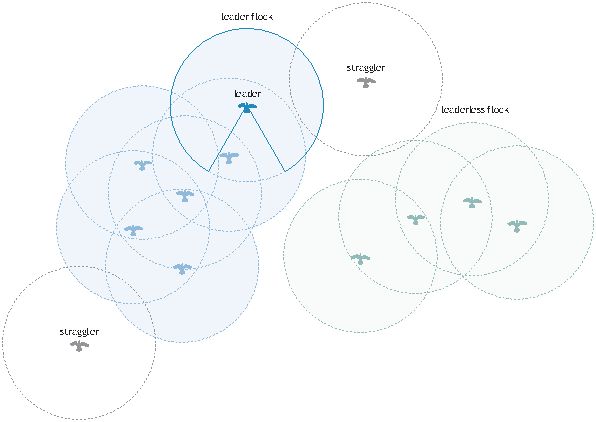
\includegraphics{fig_flock}
	\caption{A leader flock, a leaderless flock and two stragglers. Dashed lines represent the range of potential influence. The shaded areas thus encompass the animats that potentially influence each other and therefore represent the flocks' extents. The solid line in the leader flock represents the visual volume of the leader and shows that even though it potentially influences other members of the flock it is not influenced by any of them.}
	\label{fig:flock}
\end{figure}

With such an interpretation one can distinguish between \emph{flocks} and \emph{stragglers}, where the latter are animats that are not members of any flock. Moreover, by taking into account the perception model used, one can distinguish also between \emph{leader flocks} and \emph{leaderless flocks}. I interpret a leader flock as a flock with at least one \emph{leader} (\ie\ animat that is \sidenote{not}{v1.1.20050210 [FHH]: how about a democratic flock?} influenced by any of its flockmates, but influences at least one), whereas a leaderless flock is a flock with no leader (\ie\ each animat is influenced by at least one of its flockmates). 

It should be noted that these definitions represent merely a first-order approximation, but even though they might not be accurate enough from an ornithologist's point of view, they are sufficiently accurate from an algorithmic point of view. It should also be noticed that they in no way suggest or assume the existence of a single and absolute leader, in the sense of a military marching formation. Indeed, as Pomeroy and Heppner \cite{pomeroy:1992} reported, when pigeons make a turn, the birds change position so that a bird at the head of a flock will be in the rear of the flock if the flock turns \ang{180}. Therefore the hypothetical absolute leader would be at the side or rear of the flock after a turn, which means that such a model may not be appropriate at all. 

The distinction between leader flocks and leaderless flocks was introduced only to help algorithmic evaluation of the simulated behaviour. Because most real birds have a very good vision to the rear, with the exception of a blind spot directly to the rear, it is very likely that a bird at the head end of a flock will be influenced by trailers. It is thus sound to assume that in nature mostly leaderless flocks exist and if the animats are to display natural looking behaviour, there should be mostly leaderless flocks.

Let the digital universe consist of $n$ animats. Recall from sections~\ref{sec:animat}, \ref{subsec:animat:cwr}, \ref{subsec:animat:fhh}, and \ref{sec:fuzzyAnimat:afd} that in all of the study cases $q_i=\langle \vect{p}_i, \vect{v}_i, s \rangle$ denotes the current state of animat $i$, where $\vect{p}_i \in \E$ and $\vect{v}_i \in \E$ denote the animat's current position in space and velocity, for all $i=1,\ldots,n$. In addition, recall that the current perceivable state of the universe is given as $u=\langle y_1,\ldots,y_n\rangle$ and that the current perceivable data about animat $i$ is $y_i=\lambda(q_i)=\langle\vect{p}_i,\vect{v}_i\rangle$, for all $i=1,\ldots,n$. 

Let $\xi_j$ denote the maximal distance between the observed animat and another animat that still allows a `potential direct influence' between them (\ie\ the maximal distance of animat $i$ such that it might still be perceived as relevant by at least one of the perception functions of the observed animat $j$). Then, based on the current perceivable state of the universe $u$, the set $\set{M} \subseteq \set{Y}^n \times \set{Y}^n$, which represents the relation of \emph{potential direct influence} between animats, can be computed
%
\begin{equation}
	\set{M}=\left\{ (j,i)|\ j, i \in \N_n,\ \left\|\vect{p}_i-\vect{p}_j\right\| \leq \xi_j \right\}. \label{eq:metric:M}
\end{equation}

Recall that $r_\textnormal{s}$, $r_\textnormal{a}$ and $r_\textnormal{c}$ denote the separation, alignment and cohesion perception distances of Reynolds's digital bird (definition~\ref{def:animat:s:cwr}). Then, since in Reynolds's case all digital birds are created equal, $\xi_j=\max(r_\textnormal{s},r_\textnormal{a},r_\textnormal{c})$, for all $j \in \N_n$. Similarly, recall that $r_\textnormal{v}$ denotes the visual range of the fuzzy digital bird (definition~\ref{def:fuzzyAnimat:s:afd}) and since in my case all digital birds are also created equal $\xi_j=r_\textnormal{v}$, for all $j \in \N_n$. Therefore the relation of potential direct influence is in fact a set of ordered index pairs $(j,i)$, where animat $i$ is close enough to be treated as relevant by at least one of the perception functions of animat $j$. 

Let $g=g_0\ldots g_m$, where $g_i \in \N_n (i=1,\ldots,m)$, denote a series of indexes. The set representing the relation of \emph{potential direct or indirect influence} between animats is then defined as
%
\begin{equation}
	\set{M}^\star= \left\{ (j,k)|\ j, k \in \N_n,\ \exists g \right(g_0=j, g_m=k,\ (g_{i-1}, g_i) \in \set{M}, \forall i \in \N_m\left) \right\}. \label{eq:metric:M*}
\end{equation}

For all $j=1,\ldots,n$ let $\set{G}_j$ denote the set of indexes of animats that potentially directly or indirectly influence animat $j$ or are potentially directly or indirectly influenced by it. Then $\set{G}_j$ is defined as
%
\begin{equation}
	\set{G}_j=\left\{k|\ k \in \N_n,\ \left((j,k) \in \set{M}^\star\ \mathrm{or}\ (k,j) \in \set{M}^\star\right) \right\}. \label{eq:metric:Gi}
\end{equation}

Let a straggler be an animat that is neither potentially directly or indirectly influenced by any other animat nor does it potentially directly or indirectly influence any of them, and let a flock be a set of animats that potentially directly or indirectly influence one or another. Then the set of stragglers is defined as 
%
\begin{equation}
	\set{S}=\left\{ \set{G}_j|\ \left|\set{G}_j\right|=1 \right\}, \label{eq:stragglers}
\end{equation}
%
and the set of flocks as
%
\begin{equation}
	\set{F}=\left\{ \set{G}_j|\ \left|\set{G}_j\right|>1 \right\}. \label{eq:metric:flocks}
\end{equation}

As discussed in subsection~\ref{subsec:birdFlocks:fhh}, one of the key questions when studying bird flocks is the existence or necessity of a leader \cite{heppner:1997}. \sidenote{Let a leader be an animat that is a member of a flock but is not directly affected by any of the flock's members.}{v1.1.20050210 [FHH]: biologically not very likely.} In other words, a leader is an animat that is a member of a flock but all of its perception functions find all members of the flock irrelevant. However, since it is a member of the flock, the animat has a potential direct or indirect influence on at least one another member of the flock. 

Let $j$ be the index of the observed animat and let the perceived state of the universe be $u$. Then the input of animat $j$ is $x=u$.
As the fuzzy animat is a generalization of the crisp animat (see \chaptername~\ref{ch:fuzzyAnimat}), a crisp perception function (definition~\ref{def:animat:Pi}) can be represented as a fuzzy perception function (definition~\ref{def:fuzzyAnimat:Pi}) and it is safe to assume that the animat's $k$ perception functions return $k$ fuzzy neighbourhoods denoted $\fset{P}_1,\ldots,\fset{P}_k$. Recall that $\fset{P}_i=\langle\fset{N}_i,\fset{O}_i\rangle \in \fpowset{\set{P}^{\mathrm{c}_i}}$, for all $i=1,\ldots,k$. In addition recall that $\fset{N}_i \in \fpowset{\N_n}$ denotes the fuzzy set of indexes of animats that are according to characteristic $\mathrm{c}_i$ relevant to the observed animat. Let $\fset{N}_j$ denote the set $\fset{N}_1 \cup \cdots \cup \fset{N}_k$, then animat $j$ is a leader if and only if $\mu_{\fset{N}_j}(i)=0\ \forall i \in \N_n, i \neq j$ and the set of leader flocks is defined as 
%
\begin{equation}
	\set{F}_\textnormal{L}=\left\{ \set{G}|\ \set{G} \in \set{F},\ \exists j \in \set{G}\left(\mu_{\fset{N}_j}(i)=0\ \forall i \in \N_n, i \neq j\right) \right\}. \label{eq:metric:FL}
\end{equation}

\begin{definition}
	\label{def:metrics}
	Let $\set{S}(t)$, $\set{F}(t)$ and $\set{F}_\textnormal{L}(t)$ denote the sets of stragglers, flocks and leader flocks computed from the perceivable state of the universe at the discrete time step $t \in \set{T}$. Then equations~\eqref{eq:metrics0}--\eqref{eq:metrics2} are metrics of the \emph{number of stragglers}, the \emph{number of flocks} and the \emph{proportion of leaderless flocks} at the discrete time step $t \in \set{T}$.
	%
	\begin{equation}
		s(t)=\left|\set{S}(t)\right|, \label{eq:metrics0}
	\end{equation}
	\vspace*{-6mm}
	\begin{equation}
		f(t)=\left|\set{F}(t)\right|,
	\end{equation}
	\vspace*{-2mm}
	\begin{equation}
		f_\ell(t)=1-\frac{\left|\set{F}_\textnormal{L}(t)\right|}{f(t)}. \label{eq:metrics2}
	\end{equation}
\end{definition}

When measuring and judging the flocking behaviour of a group of animats one should first estimate their flocking ability and then the resemblance of their behaviour to that seen in natural flocks. The best choice to estimate the flocking ability is to turn to counting the cumulative number of collisions between animats and to observe the temporal dependency of the number of stragglers and the number of flocks. \sidenote{Since collisions in nature occur rarely, the metrics of cumulative collisions is fairly important and the lower it is, the better the flocking ability.}{v1.1.20050210 [FHH]: but you could have a group -- a swarm -- in which collisions were low, but there would be no coordination -- hence not a flock.} On the other hand, when observing the temporal dependency of the number of flocks the temporal dependency of the proportion of leaderless flocks should always be monitored as well.

A common anomaly when simulating natural phenomena is the lack of similarity to the real thing. For this reason the resemblance of the behaviour of a group of animats should always be compared to that seen in natural flocks. A classical work on the behaviour of flocks and flock formations in general is that of \sidenote{Heppner \cite{heppner:1974a}}{v1.1.20050210 [FHH]: mygoodness! a classical work! I'm flattered.} and thus when estimating the resemblance of the simulated behaviour to that seen in nature, it seems safe to turn to visual inspection of the emerged flocks and their comparison to those presented in Heppner's work (see \chaptername~\ref{ch:birdFlocks}). In addition to that it seems the best option to turn also to observing the temporal dependency of the average nearest neighbour distance and the flight direction and flight speed standard deviations in flocks. Indeed these metrics are the ones that are the most commonly employed by ornithologists \cite{gould:1974,heppner:1985,pomeroy:1992}.

%----
\section{Experiments}
\label{sec:analysis:comparison}
I compared my fuzzy model with Reynolds's through \sidenote{three sets of experiments.}{v1.0.20050124 [MM]: list experiments.} I wanted to estimate the flocking ability of the simulated birds and the resemblance of the displayed behaviour to that seen in natural flocks. 

When estimating the flocking ability I turned to counting the number of animat to animat collisions, the dynamics of the number of stragglers, the dynamics of the number of flocks, and the dynamics of the proportion of leaderless flocks. 

On the other hand, when estimating the resemblance of the simulated flocks to natural flocks I turned to visual inspection of the emerged flight formations (see \figs~\ref{fig:lineFormations} and \ref{fig:clusterFormations}) as well as the presence of the somewhat erratic, unsystematic behaviour seen in natural flocks \cite{heppner:1990}. \sidenote{I also estimated the level of alignment in flocks by measuring the flight speed and flight direction standard deviations.}{v1.1.20050210 [FHH]: probably a good start.} Furthermore I also observed the degree of uniform distribution by measuring the nearest neighbour distances. 

%--
\subsection{Flocking Ability}
In the first set, which consisted of eight experiments, 100 animats were initially placed at random locations having random flight directions and flight speeds.\footnote{Animated versions of the experiments are available in MPEG-4 format on the appended DVD-ROM.} In this set of experiments I was primarily interested if the animats are able to self-organize in flocks. To help self-organization (\ie\ allow animats to eventually meet other animats) I confined the animats using an invisible boundary (see green circle in \fig~\ref{fig:exp:01:01}). Whenever an animat passed this boundary it was forced to turn and eventually return into the confinement without changing its flight speed. In a way this resembles modelling the roosting area used by Heppner  \cite{heppner:1990} (see subsections~\ref{subsec:birdFlocks:fhh} and \ref{subsec:animat:fhh}). 

\begin{table*}[!t]
	\footnotesize\renewcommand{\arraystretch}{1}
	\setlength{\tabcolsep}{0pt} % force 0pt intracolumn separation
	\newlength{\halfw}\setlength{\halfw}{.5\linewidth-3.5pt}
	\begin{minipage}[t]{\halfw}
		\begin{tabular}{>{\centering}b{.08\halfw}>{\centering}b{.23\halfw}>{\centering}b{.23\halfw}>{\centering}b{.23\halfw}>{\centering}b{.23\halfw}}
			\toprule
			\multicolumn{5}{c}{Reynold's model} \tabularnewline
			& collisions & stragglers & flocks & proportion of leaderless flocks (avg) \tabularnewline
			\midrule
			01 & 17 & 2 & 2 & 29\pm19 \tabularnewline
			02 & 25 & 2 & 5 & 30\pm17 \tabularnewline
			03 & 14 & 2 & 5 & 29\pm18 \tabularnewline
			04 & 14 & 2 & 5 & 27\pm18 \tabularnewline
			05 & 13 & 0 & 5 & 23\pm19 \tabularnewline
			06 & 10 & 1 & 4 & 31\pm18 \tabularnewline
			07 & 14 & 4 & 6 & 23\pm16 \tabularnewline
			08 & 18 & 7 & 5 & 26\pm16 \tabularnewline
			\midrule
			avg & 15.63\pm4.5 & 2.5\pm2.14 & 4.63\pm1.19 & 26.89\pm17.49 \tabularnewline
			\bottomrule
		\end{tabular}
	\end{minipage}
	\hfill
	\begin{minipage}[t]{\halfw}
		\begin{tabular}{>{\centering}b{.08\halfw}>{\centering}b{.23\halfw}>{\centering}b{.23\halfw}>{\centering}b{.23\halfw}>{\centering}b{.23\halfw}}
			\toprule
			\multicolumn{5}{c}{fuzzy model} \tabularnewline
			& collisions & stragglers & flocks & proportion of leaderless flocks (avg) \tabularnewline
			\midrule
			01 & 0 & 1 & 6 & 83\pm14 \tabularnewline
			02 & 1 & 0 & 3 & 77\pm14 \tabularnewline
			03 & 14 & 0 & 3 & 90\pm12 \tabularnewline
			04 & 0 & 0 & 3 & 80\pm14 \tabularnewline
			05 & 0 & 1 & 5 & 82\pm17 \tabularnewline
			06 & 8 & 0 & 2 & 83\pm17 \tabularnewline
			07 & 0 & 0 & 3 & 77\pm15 \tabularnewline
			08 & 0 & 0 & 6 & 84\pm22 \tabularnewline
			\midrule
			avg & 2.88\pm5.28 & 0.25\pm0.46 & 3.88\pm1.55 & 82.26\pm16.4 \tabularnewline
			\bottomrule
		\end{tabular}
	\end{minipage}
	\caption{A comparison of the number of collisions, number of stragglers and number of flocks after 3000 simulation steps and the overall average proportion of leaderless flocks in the eight experiments used for the estimation of flocking ability for Reynolds's \cite{reynolds:1999} model and my fuzzy model. Note that because in Reynolds's case the area of potential influence is larger, the number of flocks is lower to begin with, so the values cannot be directly compared.}
	\label{tab:exp:01}
\end{table*}

\begin{figure}[p]
	\null\vspace*{1mm}
	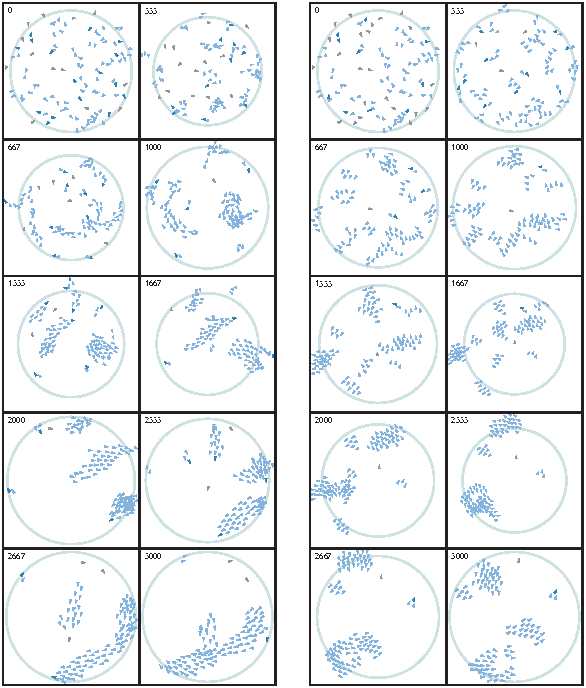
\includegraphics{fig_exp0101}
	\par\vspace*{1mm}
	\caption{A comparison of a series of time-equidistant frames from one of the eight experiments for the estimation of flocking ability for Reynolds's model \cite{reynolds:1999} (left) and my fuzzy model (right). The triangles represent animats, with the apex indicating the flight direction, and the green circle surrounding the animats represents the roosting boundary. Whenever an animat crosses this boundary it is forced to turn and eventually return into the roosting area. For reasons of print clarity the animats' images have been enlarged, which means that their apparent overlapping does not necessarily imply a collision. Furthermore, grey triangles depict stragglers, blue triangles flocking animats and dark blue triangles flock leaders. Orange triangles represent colliding animats.}
	\label{fig:exp:01:01}
\end{figure}
\afterpage{\clearpage}

My animats were strikingly good at avoiding collisions and self-organizing in flocks. While in my case in most cases no collisions occurred, Reynolds's model, summed over the whole population of 100 animats, averaged 15.63\pm4.5 collisions in 3000 simulation steps (see \tab~\ref{tab:exp:01}). In my case I also noticed that, when collisions did occur, they occurred in short periods of time (\eg\ 10 collisions in 200 simulation steps in experiment 03) and were caused by extreme proximity of animats and could be interpreted as side bumping. In Reynolds's case, however, collisions occurred randomly throughout the simulation and were mostly head-on collisions, caused by the merging of flocks. 

\begin{figure*}[!t]
	\null\vspace*{2mm}
	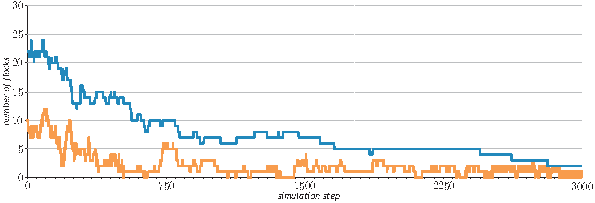
\includegraphics[width=\figurewidth]{chart_exp0101flocks_cwr}
	\par\vspace*{2mm}
	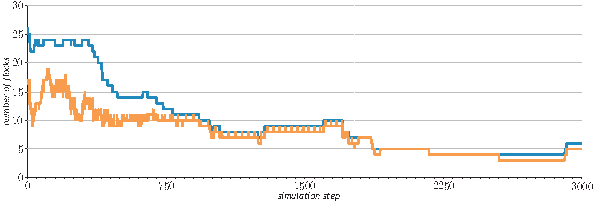
\includegraphics[width=\figurewidth]{chart_exp0101flocks_afd}
	\par\vspace*{2mm}
	%\infigurecaption{Note that because in Reynolds's case the area of potential influence is larger, the number of flocks is lower to begin with, so the values cannot be directly compared. However, since the number of flocks in both cases decreases through time it can be concluded that the two models present flocking ability. Beside this, it can also be noticed that the fuzzy model produces mostly leaderless flocks whereas Reynolds's model mostly leader flocks.}
	\caption{Plot of the number of flocks (blue line) and the contribution of leaderless flocks (orange line) for one of the eight experiments used to estimate the flocking ability of Reynolds's model \cite{reynolds:1999} (top chart) and my fuzzy model (bottom chart). Note that because in Reynolds's case the area of potential influence is larger, the number of flocks is lower to begin with, so the values cannot be directly compared. However, since the number of flocks in both cases decreases through time it can be concluded that the two models present flocking ability. Beside this, it can also be noticed that the fuzzy model produces mostly leaderless flocks whereas Reynolds's model mostly leader flocks.}
	\label{chart:exp:01:01:flocks}
\end{figure*}

Looking at the simulations in real-time I noticed that in my case both classes of flock formations (\ie\ line and cluster formations) emerged, but mostly front cluster ones. Line formations in this set of experiments did not persist for long periods of time. On the other hand, in Reynolds's case the majority of the emerged flocks was of the extended cluster formation whereas line formations did not emerge at all. 

Figure~\ref{chart:exp:01:01:flocks} presents a plot of the number of flocks in experiment 01 for my and Reynolds's model. By comparing the proportion of leaderless flocks it can be noticed that in my case mostly leaderless flocks exist, whereas in Reynolds's case mostly leader flocks exist. This tendency was also noticed in the rest of the experiments (see \tab~\ref{tab:exp:01}). 

The fact that in Reynolds's model mostly leader flocks emerge is, in my opinion, primarily caused by the perception model used in OpenSteer v0.8 (\ie\ three distinct visual volumes -- one per drive; see subsection~\ref{subsec:animat:cwr}). Not only that the combined perception volume (\figs~\ref{fig:perception:cwr}, \ref{fig:perception:afd} and \ref{fig:perception}) gives the animat a two times larger blind area than my model, it also gives the animat a much larger blind area than the values reported by Heppner \etal\ \cite{heppner:1985}. 
%
\begin{figure}
	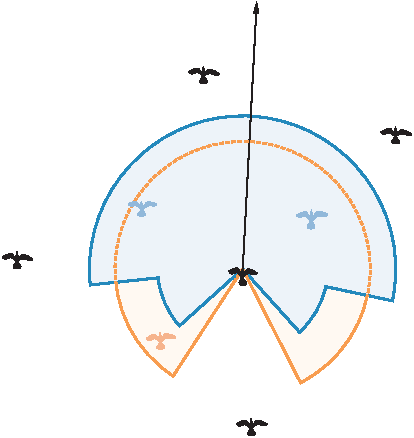
\includegraphics{fig_perception}
	\caption{Comparison of the combined perception volume that Reynolds used in the OpenSteer v0.8 implementation of his model \cite{reynolds:1999} (blue line) and the visual perception volume used in my model (orange line).}
	\label{fig:perception}
\end{figure}
%
As a result it is relatively common that a trailing animat enters the followed animat's blind area and consequently does not influence it any more. The followed animat thus becomes the trailer's leader. Since it is not influenced by any of the flockmates, the leading animat, because no random local disturbances are modelled, keeps its flight speed and flight direction while all of the flockmates only regulate their flight directions and flight speeds to follow it. Therefore, if not confined, the group will eventually form a regularly distributed and stable extended cluster formation (see frames 556--1000 in \fig~\ref{fig:exp:02:14} and 1333--2000 in \fig~\ref{fig:exp:03:01}). According to Heppner \cite{heppner:1974a}, the extended cluster formations in nature may simply be bird aggregations in which birds are flying independently toward a common destination. One might be tempted to conclude that this is precisely what is being experienced here. However, as Heppner states \cite{heppner:1974a}, extended clusters tend to be rather disorganized, with frequent breakoffs and shifts of position, but these features are not to be seen in the leader flocks that emerge from Reynolds's model. This is why I find Reynolds's use of three distinct visual volumes questionable.

%--
\subsection{Cluster Flocks}
In the second set of experiments I was interested if from an initial globular cluster formation, where all animats have the same flight speed and flight direction, natural looking flocks emerge. In this set of experiments no roosting area was modelled. However, I used three initial distribution patterns (see \fig~\ref{fig:exp:02:ini}), for which I changed the nearest neighbour distance (approximately two, four and six body lengths) and initial flight speed (10\%, 50\% and 90\% of maximum flight speed). In other words, there were 27 initial states in all.\footnote{Animated versions of the experiments are available in MPEG-4 format on the appended DVD-ROM.}

\begin{figure}
	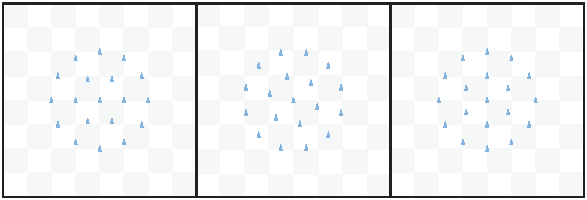
\includegraphics{fig_exp02ini}
	\caption{Initial globular cluster distribution patterns used in the second set of experiments.}
	\label{fig:exp:02:ini}
\end{figure}

Figure~\ref{fig:exp:02:14} presents a comparison of a series of time-equidistant frames from one of the experiments. 
%
\begin{figure}[!ht]
	\null\vspace*{1mm}
	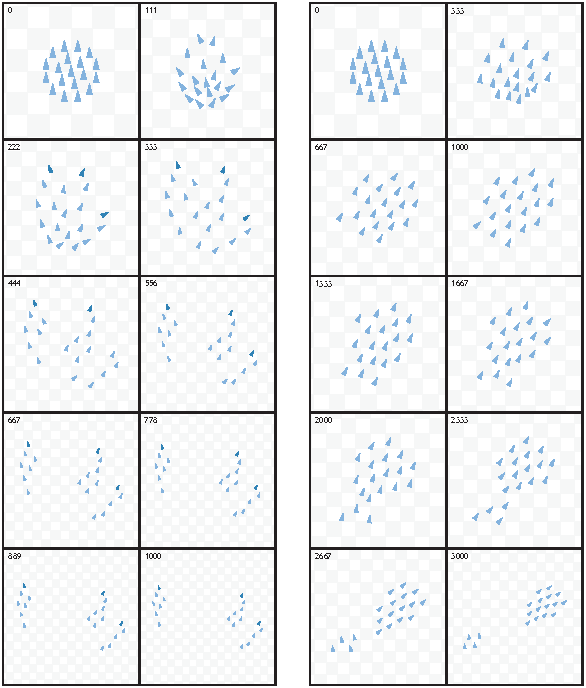
\includegraphics{fig_exp0214}
	\par\vspace*{1mm}
	\caption{A comparison of a series of time-equidistant frames from one of the 27 experiments with a globular cluster initial formation for Reynolds's model \cite{reynolds:1999} (left) and my fuzzy model (right). The triangles represent animats, with the apex indicating the flight direction. The light grey checker board represents a measurement aid with a tile being five body lengths in size. The animats' images have been enlarged for reasons of print clarity and their overlapping does not necessarily represent a collision. Furthermore, blue triangles depict flocking animats and dark blue triangles flock leaders.}
	\label{fig:exp:02:14}
\end{figure}
%
In Reynolds's case in most of the experiments one stable leader flock of the extended cluster formation emerged, which, in the 10000 simulation steps, stabilized flying at exactly maximum speed with the nearest neighbour distance matching the visual range used for the separation drive. The emerged flocks were regularly distributed and highly stable with no position shifting, which is, as already mentioned, the opposite of what can be seen in nature. In the rare cases when position shifting occurred, it originated from the centre of the flock, subsided fast, and the flock stabilized immediately afterwards. The initial flock on average broke off to 1.3\pm0.61 flocks and 0.44\pm1.09 stragglers, with the first breakoff occurring at simulation step 500\pm395.85. 

In my case the initial flock on average broke off to 2.33\pm0.83 flocks and no stragglers, with the first breakoff occurring in simulation step 3838.96\pm1680.98. In all cases the animats from the initial flock formation started shifting positions and changing flock formation. The emerged front cluster formations were stable, but when animats, due to position shifting and somewhat erratic and unsystematic behaviour, reorganized into an extended cluster formation, they usually became disorganized and eventually broke off. With breakoffs flock formations from both major classes emerged. The resulting stable cluster flocks were of the front, globular and in few cases even extended cluster formation. The extended cluster formations were disorganized with frequent shifts of position. On the other hand, the resulting stable line flocks were of the `V', echelon and inverted `V' formation. In all cases these flocks were small, consisting of only two or three members and, with the only exception of the inverted `V' formation, they were all leader flocks. The above described behaviour is strikingly similar to natural flocks. If this bears up in future work it will make a very important point. In fact, all previous hypotheses about `V' formation flight assume a functional advantage: aerodynamics \cite{badgerow:1981,badgerow:1988,hainsworth:1987,hainsworth:1989,lissaman:1970}, visibility \cite{heppner:1974a,heppner:1985}, communication \cite{gould:1974,heppner:1974b}, and kinship structure \cite{andersson:2004} (for a review, see \cite{heppner:1997,speakman:1998}). \sidenote{The behaviour present in my experiments seems to suggest instead that even the `V' formation might be an emergent property.}{v1.1.20050210 [FHH]: wow! who would have thought it.}

%--
\subsection{Line Flocks}
In the third set of experiments I was interested if from a front line formation, where all animats have the same flight speed and flight direction, line formation flocks emerge. In this set of experiments no roosting area was modelled. However, I used three initial distributions in which the animats were evenly spaced (approximately two, four and six body lengths) and I changed the initial flight speed (10\%, 50\% and 90\% of maximum flight speed). In other words, there were nine initial states in all.\footnote{Animated versions of the experiments are available in MPEG-4 format on the appended DVD-ROM.}

Figure~\ref{fig:exp:03:01} presents a comparison of a series of time-equidistant frames from one of the experiments. 
%
\begin{figure}[!ht]
	\null\vspace*{1mm}
	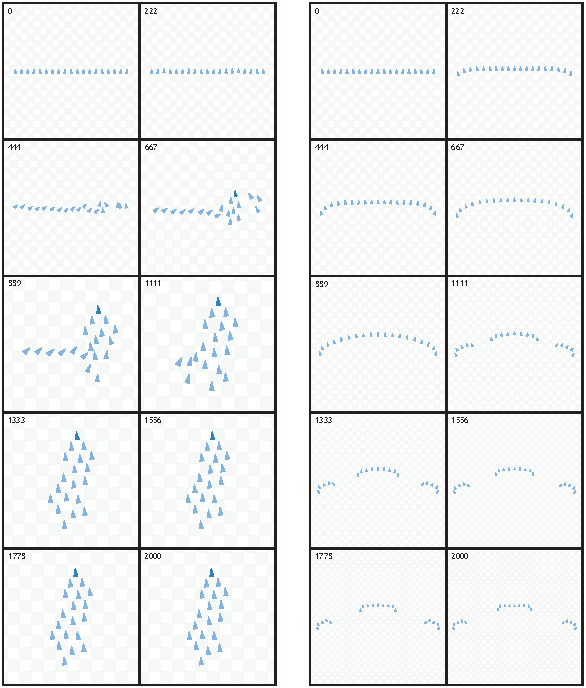
\includegraphics{fig_exp0301}
	\par\vspace*{1mm}
	\caption{A comparison of a series of time-equidistant frames from one of the nine experiments with an initial line formation for Reynolds's model \cite{reynolds:1999} (left) and my fuzzy model (right). The triangles represent animats, with the apex indicating the flight direction. The light grey checker board represents a measurement aid with a tile being five body lengths in size. For reasons of print clarity the animats' images have been enlarged, which means that their apparent overlapping does not necessarily imply a collision. Furthermore, blue triangles depict flocking animats and dark blue triangles flock leaders. Notice that in the fuzzy model the ends of the flock trail away in a curve, which is a very natural behaviour.}
	\label{fig:exp:03:01}
\end{figure}
%
In Reynolds's case the initial flock broke off on average to 1.78\pm1.3 flocks and 1\pm1.8 stragglers and there were 0.33\pm0.5 collisions. Most of the emerged flocks were of the extended cluster formation, regularly distributed and highly stable with no position shifting, but in some rare cases stable, regularly distributed column line formations emerged too. All of the emerged flocks were flying at maximum speed. In my case, on the other hand, the initial flock broke off on average to 3.22\pm0.83 flocks and 1.11\pm1.17 stragglers with no collisions. \sidenote{All of the emerged flocks were of a formation that is similar to the `V' and front line formation -- a \emph{`U'} line formation -- flying at approximately 71\% of maximum speed.}{v1.1.20050210 [FHH]: this is remarkable -- there are aerodynamic reasons for predicting something like this, but this is amazing -- anyway to play with this and get a `V' rather than a `U'?} This behaviour is very surprising. As already stated, all previous hypotheses assume a functional advantege of `V' formation flight (for a review, see \cite{heppner:1997,speakman:1998}), with the most pronounced one being energy saving due to aerodynamic reasons. However, even though the latter is supported both theoretically and empirically \cite{badgerow:1981,badgerow:1988,hainsworth:1987,hainsworth:1989,lissaman:1970,speakman:1998}, it still cannot be supported undisputedly. Mostly because not all large long-distance migrants use formation flight and furthermore because some birds often use acute `V' formations, where the trailing birds, in contrast with the bird at the head of the formation, may make substantial energy savings, while others use more obtuse or bow formations, in which the bird at the head is only a little ahead of its neighbours, and energy savings are probably more equable \cite{andersson:2004}. It is thus impressive that in my experiments, where no aerodynamical aspects as well as no kinship relations \cite{andersson:2004} are taken into account, `U' formations emerge. If by any chance in future work, after the inclusion of a proportion of informed individuals \cite{couzin:2005}, `V' formation flocks will emerge this will represent a remarkable discovery.


 	% !TeX root = ./thesis.tex










%==============================
\chapter{Conclusion}
\label{chap:conclusion}

%-----
\EBlettrine{The} phenomenon known as collective animal behaviour is one of the most beautiful spectacles one can observe in nature. Although researched and analysed by scientists from many disciplines and perspectives it is still puzzling in many ways. Examples of such puzzling questions are why did collective behaviour (especially highly organized forms) evolve and why do we see so much variation in behaviour even in closely related species. Through the construction of a genetic fuzzy system capable of evolving various forms of collective behaviour this study represents an attempt in shedding additional light on potential reasons why highly organized collective behaviour evolved.

We started the study by expanding on a known fuzzy model \cite{lebarbajec2005fuzzy,lebarbajec2005simulating} for the purpose of studying predator-prey dynamics in hand-crafted models. Prey animats in this model \cite{demsar2014simulated} could exhibit two types of behaviour -- a social one where they actively strived for grouping (via cohesion and alignment drives) and an individualistic one where they did not. We focused on vision as the principal means of perception, took into account occlusion \cite{kunz2012simulations} and working memory limitations \cite{ballerini2008interaction,engle1999individual,sherry1989hippocampus}, and considered three target selection (predation) tactics. With the first tactic predators attacked the nearest out of visible prey individuals, with the second the most visually isolated prey individual out of the visible ones, and with the third the centre of the visible group (visible prey individuals). To achieve biological relevance we tuned the parameters based on realistic data about birds (starlings, \emph{Sturnus vulgaris}, for prey, and peregrine falcon, \emph{Falco peregrinus}, for the predator). The study suggests that the most successful predator is the one that attacks the most visually isolated individual, while the least successful predator is the one that attacks the centre of the visible group, a result similar to those reported by field observations \cite{zoratto2010aerial}. As a plus, results obtained by our study suggest that, from a prey individual's perspective, social behaviour is more advantageous than individualistic behaviour, which strengthens our belief in the hypothesis that cluster flocking might serve as be a mechanism for protection from predation.

Field observations suggest that predators in nature are able to, at least partially, overcome the defensive benefits of prey grouping by using an assortment of sophisticated hunting strategies \cite{cresswell2011predicting,forsman1998visual,gazda2005division,handegard2012dynamics,hector1986cooperative,kane2014falcons,lopez2006bottlenose,nottestad2002digging,rutz2012predator}. As the parametrization and tuning of such tactics in a hand-crafted model would be a tiresome task we developed an evolutionary model that simulates the evolution of composite target selection tactics \cite{demsar2015simulating}. The most successful predators were those that first dived deep into the centre of the nearby prey group causing chaos and dispersal of the group. Following that they targeted stragglers (individuals that in the process got separated from the rest of the group). The tactic, which we termed as the dispersing tactic, is similar in function to the tactics used by several predators in nature \cite{larsson2012why,pavlov2000patterns}. In our study predators that used the dispersing tactic came out as significantly more successful hunters in a direct competition with predators that used a mixture of simple tactics. Again a result corroborating field observations \cite{pavlov2000patterns}. However, this was true only in the case when our model took into account the possibility of predator confusion. The concept of predator confusion is based on the confusability hypothesis, which suggests that a group of visually similar prey might make it difficult for the predator to select and track its target \cite{nishimura2002predator,zheng2005behavior,kunz2006prey,olson2013predator,olson2016evolution,rutz2012predator}. A different story was the case of the prey's delayed response, a defensive manoeuvre where prey rather then escaping on first sight of the predator, delay their response to a later point in time, and then try to outsmart the predator with rapid movement \cite{partridge1982structure}. The only predators able to, at least to some degree, overcome the defensive benefits of this escape manoeuvre, were again the predators that used the dispersing tactic. Because the dispersing tactic yields higher success to predators we can assume that dispersing the group reduces the group's defensive benefits. This strengthens our belief in the hypothesis that compact groups of prey might function as a defensive mechanism from predation. The absence of an advantage of the dispersing tactic over simple predation tactics when predator confusion is not at play indicates that predator confusion might have played an important role in the evolution of advanced predation tactics, as well. All of these findings were a clear indication of potential interplay between target selection tactics and the evolution of prey group behaviour.

Several studies already pursued the artificial evolution of collective animal behaviour, most by tuning parameters of previously presented non-evolutionary models. Very few succeeded to evolve it from scratch, and even in these cases the evolved behaviour can be termed as ``crude.'' Based on presented material the successful studies portray either clumping \cite{biswas2014causes,hein2015evolution,witkowski2016emergence}, or swarming with collisions \cite{olson2013predator,olson2015exploring,olson2016evolution,witkowski2016emergence}. To study how predation tactics influence the evolution of prey behaviour we designed a novel open-ended, artificial life-like evolutionary model where the drives of individual animats are encoded via linguistic fuzzy rules \cite{demsar2017evolution}. In our genetic fuzzy system prey and predator animats coexist in a shared environment. Based on knowledge about predator target selection tactics gained from our previous research \cite{demsar2014simulated,demsar2015simulating} we designed several types of hand-crafted predators that attack evolving prey. Subsequently, in our model only the survival instincts of prey animats steer the evolution of their behaviour and collective behaviour will emerge only if it will help prey animats survive. We analysed the evolved prey behaviour and showed that based on biologically relevant metrics \cite{couzin2002collective,vicsek2012collective,tunstrom2013collective} our evolutionary model is capable of producing a wide range of behaviours, some qualitatively and visually similar to those reported by experimental studies \cite{tunstrom2013collective}. Since we used a genetic fuzzy system we were able to further analyse the evolved behaviours by studying the fuzzy rule bases that govern the actions of individual animats. Doing so we showed that when clustering the rule bases by the type of evolved behaviour and observing the average proportion of rule antecedents that contain predator related linguistic variables there exists a statistically significant difference between the rule bases. This gives us confidence in advocating that artificial life-like evolutionary modelling based on linguistic fuzzy rule-based systems could be used for answering the illusive biological questions ``why'' collective animal behaviour evolved, and due to their linguistic nature also provide a deeper insight into the ``how.''

To gain further insight into potential ``whys'' we used the newly developed genetic fuzzy system in a controlled experiment where prey evolved while subject to multiple, systematically picked predation tactics simultaneously \cite{demsar2016balanced}. The predation tactics can be split into two groups; those for which the natural defensive response of prey might be grouping and those for which the natural response might be dispersing. We classified the evolved behaviours using quantitative metrics in a similar fashion as previous studies \cite{couzin2002collective,vicsek2012collective,tunstrom2013collective}. When prey evolved while exposed to predators that adopted tactics from only one group the results of evolution corroborated with previous studies \cite{biswas2014causes,olson2013predator,olson2016evolution,wood2007evolving}; prey animats evolved either grouping or dispersing behaviour, with values of metrics characteristic for milling or swarming. When prey animats evolved while exposed to antagonistic pressures that at the same time steered the evolution towards grouping and towards dispersing we detected a significant increase of polarization in motion of prey groups. This suggest that exposure to antagonistic predation pressures might be a necessary requirement for prey individuals to evolve parallel movement. This could indicate that the direction of evolution (grouping or dispersing) is not A versus B, but a labile result -- whether grouping or dispersing evolves depends on a) the nature of the group, and b) the pressures that the group finds itself facing.

\paragraph{Limitations of this study and future work} Throughout our research we devised a number of ideas which could potentially lead to interesting future studies of collective animal behaviour. When it comes to application of evolutionary models for help with providing answers to biological questions the most obvious research advances lie in upgrades towards a higher biological relevance. Evolutionary models are usually simplified due to high computational demands of genetic algorithms and as a result the models are most often restricted to two dimensions, animats in them have unrealistic perception systems, and animats traditionally move with constant speeds, etc. To allow the animats to vary their speed in an evolutionary model we would probably need to implement some kind of fatigue system as well, so that, just like in nature \cite{norin2016measurement,roche2013finding}, animats would not be able to move with their maximum speed indefinitely.

Another possible direction would be the investigation of how heterogeneity influences the evolved behaviour. Some recent studies suggest that in an algorithm mimicking artificial evolution heterogeneous groups might evolve a different behaviour than homogeneous ones \cite{olson2015exploring}. Others suggest that heterogeneous groups might be necessary to achieve a more ``natural'' behaviour \cite{demsar2013family}, and that differences among individuals might be essential for group coordination \cite{marras2012information,marras2013schooling}. In nature heterogeneity (both in behaviour as well as in physiology) is always present, for example birds in a flock often differ in size, gender, age, and some times even species \cite{lebarbajec2009organized,jolles2013heterogeneous}. It is not uncommon that stronger members of the group are positioned at the ``safer'' parts of it \cite{hamilton1971geometry}, which leaves the weaker individuals more exposed to predator attacks. Some predators often intentionally target weak prey individuals \cite{domenici2014howsailfish,marras2015notsofast}, and by using models that consider also physiological heterogeneity one could, apart from studying its influence on prey behaviour, also study how it influences the adaptation of predator target selection tactics.

To our knowledge, in most of the existing models \cite{demsar2014simulated,demsar2015simulating,demsar2016balanced,demsar2017evolution,nishimura2002predator,zheng2005behavior}, the predator animat, once it selects its target, uses classical pursuit \cite{nahin2012chases} to chase its target. In nature some predators use advanced pursuit tactics, for example some species of falcons use the technique of motion camouflage \cite{kane2014falcons}. With this technique they either camouflage themselves against a fixed background object so that the targeted individual observes no relative motion between them and the fixed object, or they approach the targeted individual in a way that, from the targeted individual's point of view the predators always appear to be on the same bearing \cite{justh2006steering}. One possible future study might therefore be a genetic fuzzy system for the evolution of predator pursuit tactics. Or co-evolution of prey behaviour and predator pursuit tactics.

In nature predators often resort to group hunting \cite{creel1995communal,escobedo2014groupsize,fanshawe1993factors,lett2004continuous,muro2011wolfpack,packer1988evolution,scheel1991group}. Occasionally they cooperate (\ie cooperative hunting) to increase the probability of a successful hunting event \cite{creel1995communal,packer1988evolution}. Even though in our current model prey animats are often attacked by several predators at once the predators do not cooperate in any way. Studying the evolution of predator cooperation during hunting events would probably also lead to an interesting study.

Another possible upgrade would be the consideration of short term memory, which comes to play when, for example a predator moves out of view of the targeted individual (out of range or in its blind area). In current models, the targeted individual completely forgets that the predator was attacking it just a moment ago.

An important question is also flight initiation distance. In certain fish species prey as a defence mechanism delay their response \cite{partridge1982structure}. Our research already showed, that a delayed response is quite effective with certain target selection tactics. With an evolutionary model, however, we can study under what conditions (if) such a delayed reaction will emerge. Research in this this direction is already on its way, our current provisional results suggest that the answer might be related to the ratio between predator and prey speed.

The rule base is probably the most important part of a fuzzy animat since it defines the drives of the animat, which have the highest influence on the animat's behaviour. In genetic rule learning the data base of a fuzzy system is static, it does not evolve. As our genetic fuzzy system executes genetic rule learning, fuzzy variables, the linguistic terms, and the interpretation of logic connectives, which are all defined in the data base of a genetic fuzzy systems were hand-crafted. In our research this did not appear to be a limitation as our genetic fuzzy system is capable of evolving many of the forms of collective behaviour that can be commonly observed in nature.

The degree of truth for each fuzzy term is defined by its membership function, these functions come in many shapes (triangular, trapezoidal, singleton, Gaussian, etc.). Even though our algorithm supports many different types of membership functions we developed all models by means of trapezoidal/triangular functions only. These provide the lowest ratio between computational complexity and ease of conceptualization, visualization, and explanation. Again, in the case of our genetic fuzzy system the use of triangular functions did not seem to be a limiting factor as the repertoire of evolved collective behaviours is wider than in previous similar studies \cite{biswas2014causes,hein2015evolution,olson2013predator,olson2015exploring,olson2016evolution,reynolds1993evolved,sayers2009evolved,spector2003emergence,wood2007evolving}. Nevertheless, the evolution of rule bases with more sophisticated types of membership functions and the evolution of the whole fuzzy knowledge base seem like promising research directions for our future work.

To conclude, evolutionary models allowed us to untangle a number of interesting riddles related to collective behaviour already, but judging by the current trends we believe that the best is yet to come.
 	\begin{appendices}
	\end{appendices}

\backmatter
 	% !TeX root = ./thesis.tex

% use bibtex for bibliography








%==============================
\bibliography{jd}

	% !TeX root = ./thesis.tex










%==============================
\begin{razsirjeniPovzetek}

%-----
\EBlettrine{Ali} imajo jate ptic, jate rib, črede kopitarjev, roji mušic, mehiški val, trume ljudi na koncertu, borza in biološke celice kaj skupnega? S tem se ukvarjajo znanstveniki, ki raziskujejo področje skupinskega vedenja. Primere skupinskega vedenja iz narave prikazuje slika~\ref{fig:CB_si}. Skupinsko vedenje je fascinantno področje, ki analizira, kako preproste odločitve posameznikov vplivajo na dinamiko celotne skupine. Aristotel je nekoč izjavil: »Celota je več kot vsota sestavnih delov.« -- trditev, ki zelo lepo opiše bistvo skupinskega vedenja. Rezultati raziskav iz področja skupinskega vedenja so zanimivi za znanstvenike z več različnih področij, od biologije, fizike in medicine do družboslovnih ved in računalništva \cite{deisboeck2009collective,lebarbajec2009organized,nahin2012chases,silverberg2013collective,spector2003emergence,sumpter2006principles,vicsek1995novel,wei2009pursuit,xu2014crowd}.

\begin{figure}[p]
	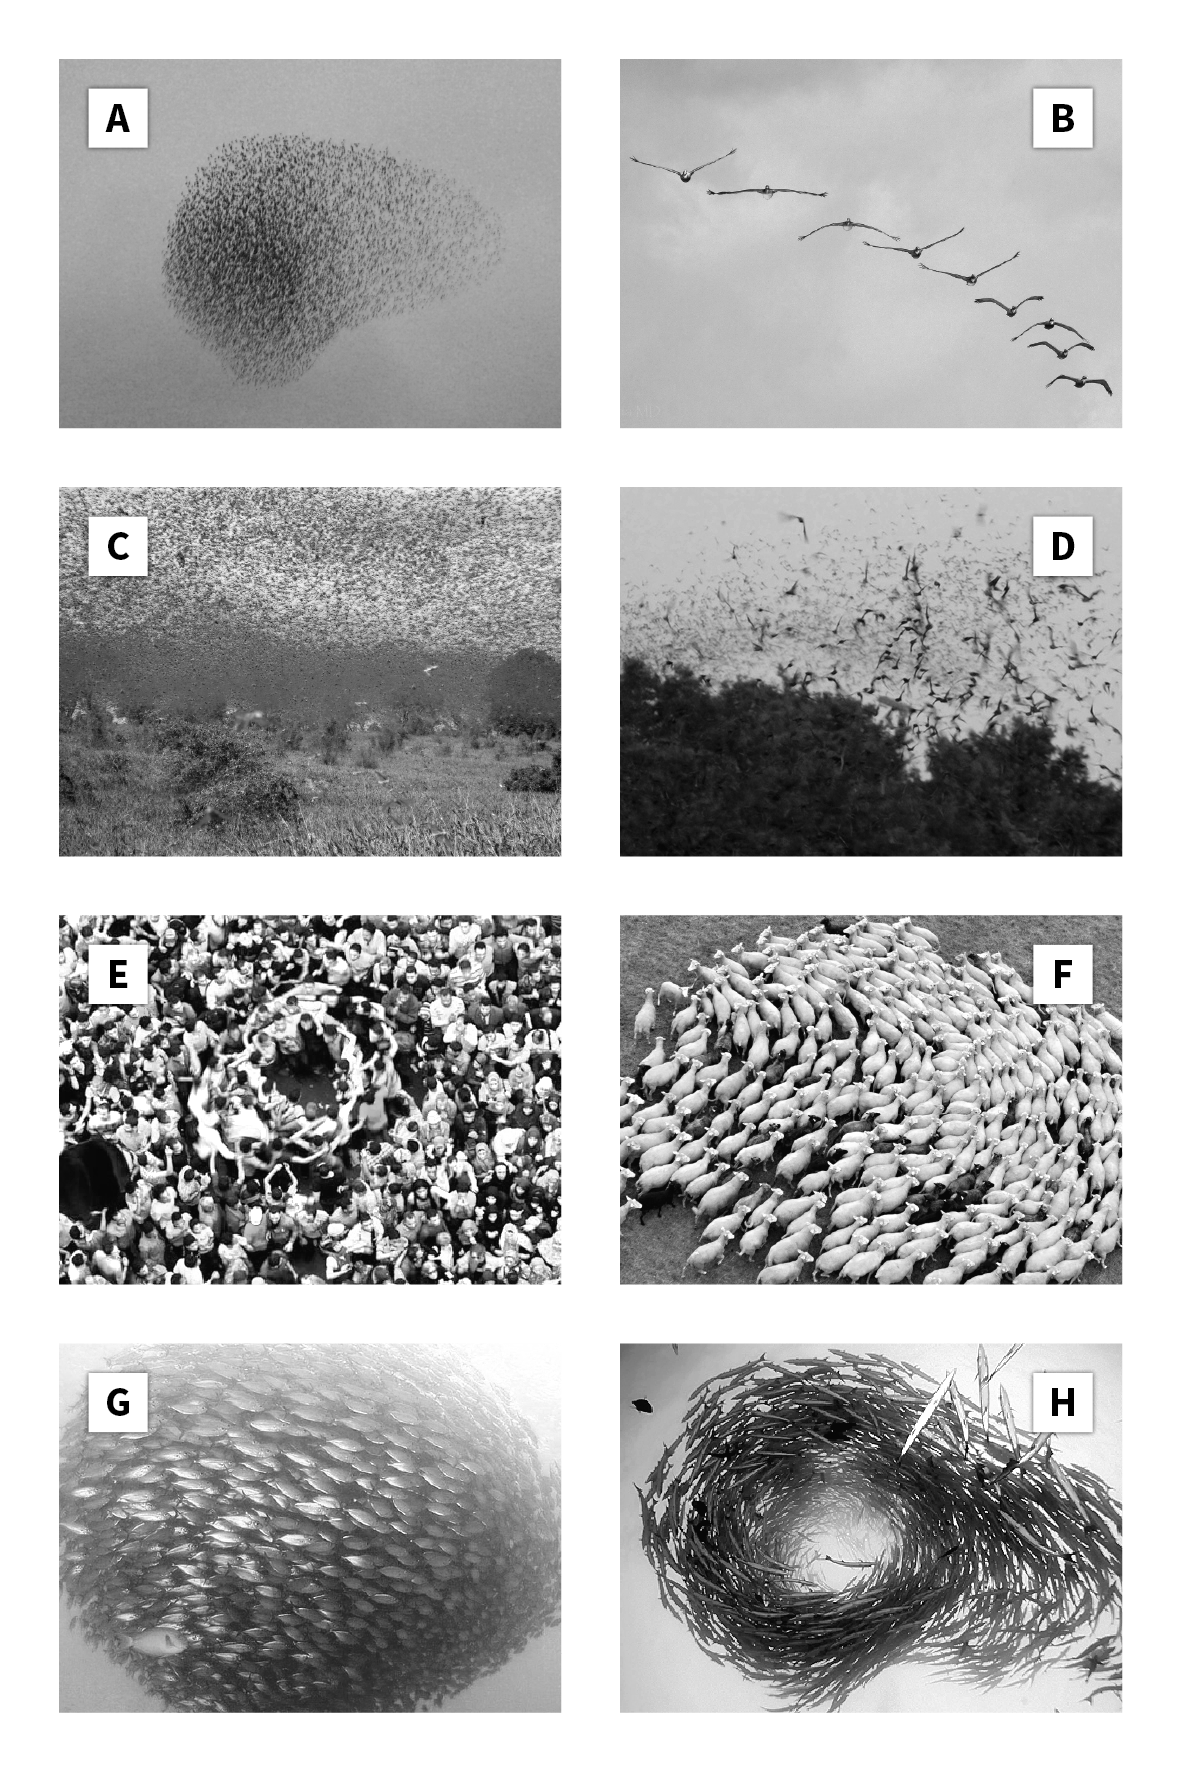
\includegraphics[width=\figurewidth]{figCB_BW.png}
	\caption{Primeri različnih režimov skupinskega vedenja, ki jih lahko opazimo v naravi. A) jata škorcev (© Tim Regan, \href{www.flickr.com}{flickr.com}). B) pelikani, ki letijo v formaciji (© Daniel D'Auria, \href{www.flickr.com}{flickr.com}). C) roj kobilic (© FAO emergencies, \href{www.flickr.com}{flickr.com}). D) roj netopirjev (© Amanda, \href{www.flickr.com}{flickr.com}). E) ljudje na koncertu (© Amanda Mustard, \href{http://www.amandamustard.com/}{amandamustard.com/}). F) čreda ovc (© Dariusz Paciorek, \href{http://www.aeroart.com.pl/}{aeroart.com.pl/}). G) ribe v jati, ki ima obliko krogle (© Bo Pardau, \href{www.flickr.com}{flickr.com}). H) kroženje rib okoli praznega jedra (© Robin Hughes, \href{www.flickr.com}{flickr.com}).}
	\label{fig:CB_si}
\end{figure}

Področje skupinskega vedenja (\angl{collective behaviour, collective animal behaviour, swarming behaviour}) je tako zelo aktualno, saj kljub temu, da gre za pojav, ki ga lahko praktično vsak dan srečamo v naravi, mnoga raziskovalna vprašanja ostajajo nerešena \cite{krause2002living,lebarbajec2009organized,sumpter2006principles}. Tako še vedno nismo povsem prepričani, zakaj se nekatere skupine živali (predvsem tiste, kjer se živali gibajo močno usklajeno) pravzaprav sploh tvorijo \cite{lebarbajec2009organized}. Zakaj v naravi obstaja toliko različnih oblik skupinskega vedenja? Zakaj zgolj nekaj vrst ptic, ki letijo v skupinah, to počne v močno usklajenih oblikah? Zakaj so si ptice, ki pripadajo sorodnim vrstam \cite{jarvis2014wholegenome}, po obliki skupinskega vedenja tako različne \cite{lebarbajec2009organized}? V literaturi o skupinskem vedenju lahko najdemo vrsto različnih, tudi nasprotujočih si hipotez o tem, zakaj se živali združujejo v skupine. Nekatere pravijo, da živali tako povečajo učinkovitost pri razmnoževanju in iskanju hrane \cite{krebs1994behavioural}, druge trdijo, da ribe in ptice z usklajenim gibanjem varčujejo z energijo \cite{hemelrijk2014increased,marras2015fish,portugal2014upwash}.

Verjetno najbolj pogosta hipoteza o skupinskem vedenju trdi, da pri živalih združevanje v skupine služi kot učinkovit obrambni mehanizem pred plenilci \cite{cresswell2011predicting,hart2005predator,krause2002living,larsson2012why,lebarbajec2009organized,nishimura2002predator,pavlov2000patterns}. Hipoteza o sebični čredi (\angl{the selfish-herd hypothesis}) trdi, da posamezne živali z združevanjem v skupine zmanjšujejo svoje območje ogroženosti \cite{hamilton1971geometry,viscido2001response}. Hipoteza o zmanjševanju tveganja (\angl{the dilution of risk hypothesis}) razlaga, da ima posameznik manjšo verjetnost, da bo izbran kot tarča plenilca v večjih skupinah \cite{tosh2011conditions}. Hipoteza mnogih oči (\angl{the many eyes hypothesis}) pravi, da se z velikostjo skupine zmanjšuje čas, ki ga mora za odkrivanje nevarnosti vsak posameznik nameniti opazovanju okolice \cite{elgar1989predator,haley2014exploring,ruxton2008application,sadedin1998influence} ter da se z večanjem skupine povečuje verjetnost pravočasne zaznave plenilca \cite{galton1871gregariousness}. Hipoteza o zmedljivosti (\angl{the confusability hypothesis}) predvideva, da ima plenilec težave pri izbiri in sledenju tarče, če se ta nahaja v skupini, ki si je medsebojno vizualno podobna \cite{demsar2015simulating,kunz2006prey,nishimura2002predator,olson2013predator,olson2016evolution,zheng2005behavior}.

Številčnost nekaterih primerkov skupin (na primer jate rib in ptic) je zelo velika in jih težko zapremo v nadzorovano okolje, kjer bi nato znanstveniki lahko preiskovali različne hipoteze o njihovem obnašanju \cite{lebarbajec2009organized}. Obenem v naravi živali prebivajo v različnih okoljih in so podvržene pritiskom različnih plenilcev, ki uporabljalo različne taktike napada. To pomeni, da težko analiziramo zgolj vpliv plenilcev na skupinsko vedenje živali brez posrednega vpliva okolja, v katerem se le-te gibljejo. Računalniški pristopi nam po drugi strani omogočajo razvoj modelov, ki so sposobni reproducirati opazovano vedenje in hkrati odstraniti nezaželene vplive okolja, ki otežujejo empirične raziskave. Prav računalniški pristopi so v zadnjem obdobju vedno bolj pogosti pri raziskovanju raznih hipotez o skupinskem vedenju \cite{vicsek1995novel,couzin2002collective,hildenbrandt2010selforganized}. Ker imajo pri računalniških pristopih znanstveniki popoln nadzor nad vsemi parametri modela, zaključki običajno ne veljajo zgolj za eno samo živalsko vrsto, ampak so lahko tudi bolj splošni.

%-----
\section{Animat}

Eden izmed računalniških pristopov k obravnavi skupinskega vedenja je gradnja modelov, zasnovanih na nivoju posameznika (\angl{individual-based models}). Pri tem pristopu raziskovalci modelirajo lokalni program, ki definira vedenje posamezne simulirane živali (animata, \angl{animat} \cite{cliff1993adding,fine2013unifying,lebarbajec2005fuzzy,watts1998animats,wilson1985knowledge}, slika~\ref{fig:animat_si}), nato pa opazujejo dogajanje pri medsebojni interakciji velikega števila animatov. Običajno je lokalni program, ki definira vedenje posameznika, načrtovan povsem ročno ter se nato skozi čas ne spreminja. To naredi programer/znanstvenik, ki nato v nadaljnjih korakih s spreminjanjem parametrov animata njegovo vedenje priredi do te mere, da slednje čim bolje ponazarja vedenje živali v naravi \cite{couzin2002collective,demsar2014simulated,demsar2015simulating,lebarbajec2005fuzzy,lebarbajec2005simulating,hildenbrandt2010selforganized,vicsek1995novel}. Pri tem si pomaga z različnimi metrikami, ki so jih raziskovalci zabeležili pri empiričnih študijah. Tako načrtovan in pripravljen model se potem s pomočjo izvajanja simulacij nad animati v nadzorovanem umetnem okolju uporabi za različne raziskave skupinskega vedenja. 

\begin{figure}
	\vskip.2in
	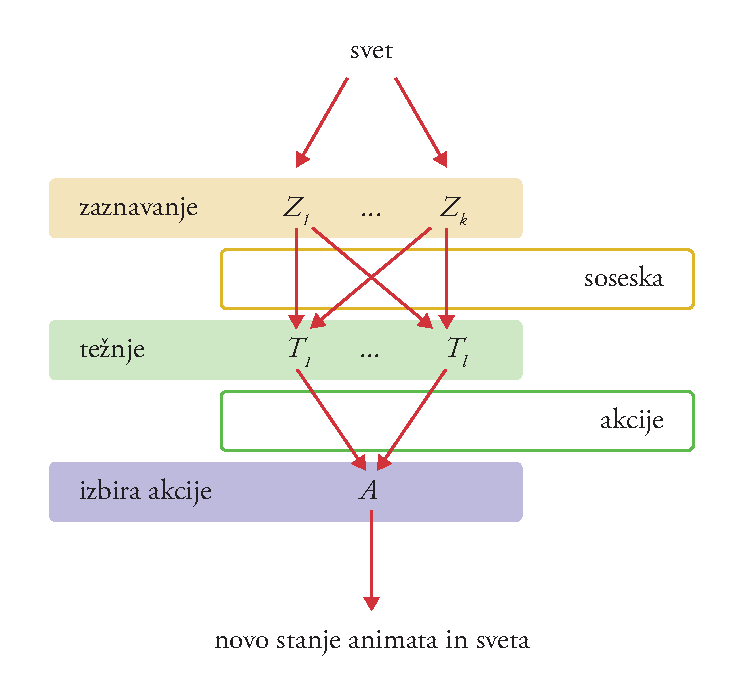
\includegraphics[width=.6\figurewidth]{fig_animat_si}
	\vskip.2in
	\caption{Vizualizacija procesov in terminologije povezanih z animatom.}
	\label{fig:animat_si}
\end{figure}

Animat torej povzema osnovne lastnosti pravih živali \cite{lebarbajec2005fuzzy}. Prav tako kot prave živali obstaja v prostoru in času, obkrožajo pa ga živi in neživi objekti, kar pomeni, da animat prebiva v nekem prostoru Animat se zaveda svojega trenutnega stanja in je sposoben zaznavanja stanja bližnje okolice. Ima težnje, ki jih preko izvajanja akcij poskuša zadovoljiti. Tako lahko preko akcij vpliva na svoje stanje ter na stanje prostora.

S pomočjo modelov, zasnovanih na nivoju posameznika, je bilo pokazano, da lahko do zapletenih dinamik skupinskega vedenja pridemo že, če posamezniki sledijo dokaj preprostim težnjam. Prvi poskusi modeliranja skupinskega vedenja s pomočjo modelov zasnovanih na nivoju posameznika segajo v osemdeseta leta prejšnjega stoletja. Aoki \cite{aoki1982simulation} je predlagal pristop od spodaj navzgor za simuliranje jat rib. Reynolds \cite{reynolds1987flocks} je razvil prvi računalniški model za proceduralno animiranje jat ptic. Podobno kot Reynolds sta tudi Heppner in Grenander \cite{heppner1990stochastic} modelirala jate ptic, a s pomočjo stohastičnih nelinearnih diferencialnih enačb. Poleg naštetih modelov se tudi večina novejših \cite{couzin2002collective,demsar2013family,demsar2014simulated,demsar2015simulating,demsar2016balanced,demsar2017evolution,helbing1995social,hildenbrandt2010selforganized,lebarbajec2009organized,parrish2002schools,schellinck2011review,sumpter2006principles,vicsek2012collective} razlikuje zgolj v implementaciji določenega segmenta animata, glavni del, ki definira vedenje, pa je v večini modelov zelo podoben. Vedenje animatov v večini primerov temelji na treh težnjah (Slika~\ref{fig:drives_si}), ki se imenujejo razmik (\angl{separation}), poravnava (\angl{alignment}) in kohezija (\angl{cohesion}). S kohezijo modeliramo težnjo biti blizu drug drugemu. Tako se animat, če nima bližnjih sosedov, želi približati tistim, ki so bolj oddaljeni. S pomočjo težnje razmika animati ohranjajo osebni prostor ter preprečujejo trke. S pomočjo poravnave usklajujejo smer in hitrost gibanja s sosedi. Ker se lahko že zgolj s poravnavo smeri gibanja prepreči razpadanje skupin ter medsebojne trke, nekateri modeli uporabljajo izključno to težnjo \cite{vicsek1995novel}.

\begin{figure*}
	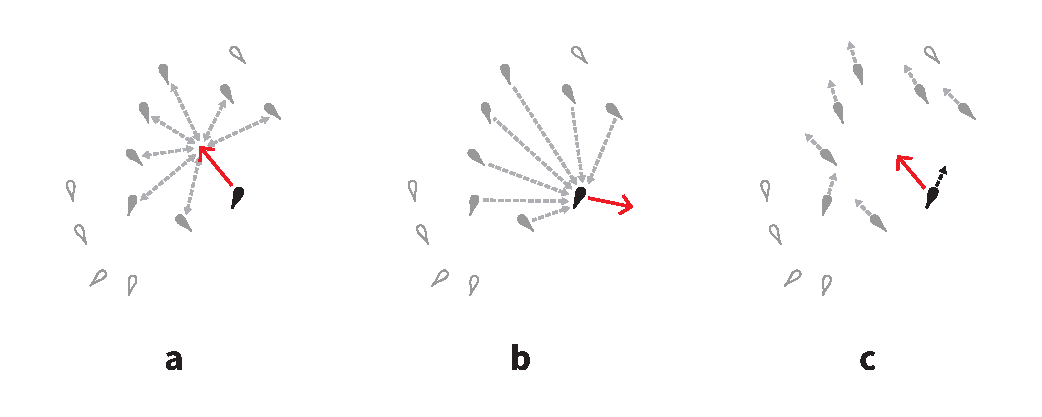
\includegraphics[width=\figurewidth]{figDrives}
	\caption{Vizualizacije treh osnovnih teženj: (a) kohezija, (b) razmik in (c) poravnava. Črni animat je opazovani posameznik. Sivi animati so sosedi, ki neposredno vplivajo na vedenje opazovanega posameznika. Beli animati s sivo obrobo so sosedi, ki nimajo neposrednega vpliva na vedenje opazovanega posameznika.}
	\label{fig:drives_si}
\end{figure*}

%-----
\section{Evolucijski animat}

Nekoliko drugačen pristop predstavljajo modeli, kjer vedenje animatov ni načrtovano povsem ročno, ampak lahko animati svoje vedenje skozi čas spreminjajo samodejno (pri ročno načrtovanih modelih se obnašanje animatov skozi čas ne spreminja). Spremembe vedenja izvajajo za dosego čimbolj učinkovitega zadovoljevanja teženj v danem okolju oziroma prostoru. Običajno so taki modeli osnovani na genetskih algoritmih, ki s pomočjo selekcije, križanja in mutacije posnemajo naravno evolucijo in tako iščejo rešitve za razne kompleksne probleme \cite{goldberg1989genetic,goldberg2002design,holland1992adaptation}. Selekcija zagotavlja, da imajo boljše rešitve oziroma boljši osebki večjo možnost za reprodukcijo. S tem se zagotovi prenos dobrega genetskega materiala v naslednje generacije. Kvaliteta posamezne rešitve se ocenjuje s pomočjo ocenjevalne funkcije. Križanje posnema izmenjavo genetskega materiala pri reprodukciji. Pri formiranju novega osebka se tako kromosomi staršev združijo v en kromosom, ki opredeljuje otroka. S tem se lastnosti staršev prenesejo na otroke. V naravi razne anomalije v reprodukcijskem procesu povzročijo spremembe v genetskem materialu, kar vodi v mutacije, zato genetski algoritmi v zadnjem koraku opravljajo še mutacije -- redke naključne spremembe otrokovega kromosoma. 

Pri najbolj pogosti uporabi genetskih algoritmov so generacije osebkov med seboj običajno povsem ločene. Pred generiranjem nove generacije se najprej oceni kvaliteta vseh rešitev v trenutni generaciji, nato pa se preko izvajanja operacij selekcije, križanja in mutacije ustvari nova enako velika generacija.

V zadnjem času je bilo obljavljenih več pomembnih člankov \cite{kunz2006prey,olson2013predator,olson2016evolution,biswas2014causes,demsar2015simulating,demsar2016balanced,demsar2017evolution,hein2015evolution}, ki so uporabili genetske algoritme za analizo različnih hipotez o evoluciji skupinskega vedenja. Nekateri izmed teh \cite{sayers2009evolved,spector2003emergence,wood2007evolving} so genetske algoritme uporabili predvsem za prilagajanje parametrov v diferencialnih enačbah, ki definirajo znane težnje (težnje izhajajoče iz ne-evolucijskih modelov). Glavna težava pristopa je, da uporaba znanih teženj verjetno usmerja tok evolucije proti razvoju znanega (skupinskega vedenja). Reynolds je bil prvi, ki je uporabil kombinacijo genetskih algoritmov in genetskega programiranja \cite{koza1992genetic} za simuliranje evolucije skupinskega vedenja, ne da bi uporabil vnaprej definirane težnje \cite{reynolds1993evolved}. Vedenje, ki se je v njegovem primeru razvilo, težko primerjamo s kompleksnimi pojavi skupinskega vedenja v naravi. Glavni razlog verjetno tiči v tem, da je bil Reynoldsov model pretirano poenostavljen. Zaera in sod. so pri poskusu simuliranja evolucije skupinskega vedenja uporabili kombinacijo umetnih nevronskih mrež in genetskih algoritmov. Njihov poskus se ni končal najbolje, saj jim ni uspelo razviti vedenja, ki bi bilo podobno primerom iz narave. Po prepričanju avtorjev je glavni razlog za spodletel poskus v ocenjevalni funkciji. Ugotovili so, da je težko definirati ocenjevalno funkcijo, ki dobro opiše pojav skupinskega vedenja s stališča posameznika. Ocenjevalna funkcija je ključni element pri genetskih algoritmih, saj določa, katere rešitve bodo v procesu evolucije vplivale na prihodnje rodove, katere pa bodo izumrle.

Ocenjevanje skupinskega vedenja s stališča posameznika je problematično vsaj z dveh stališč. Definicija stopnje oziroma kvalitete skupinskega vedenja ni najbolj jasna, tako s stališča posameznika kot skupine. V naravi namreč obstaja mnogo različnih režimov skupinskega vedenja. Vsak izmed njih je čudovit in spektakularen na svoj način. Neposredno ocenjevanje stopnje skupinskega vedenja obenem eksplicitno usmerja evolucijo proti razvoju skupinskega vedenja -- posameznike sili k izvajanju akcij, ki povečajo stopnjo skupinskega vedenja. Pri tradicionalni rabi genetskih algoritmov (ko gre za iskanje čim bolj optimalnih rešitev pri kompleksnih nalogah) takšno usmerjanje sicer ni problematično, se pa izkaže kot problematično, ko želimo uporabiti genetske algoritme za raziskovanje možnih vzrokov za razvoj skupinskega vedenja. Pri tovrstnih raziskavah nas bolj kot optimalna znana rešitev zanima, če se bo med animati skupinsko vedenje razvilo samodejno (brez eksplicitnega siljenja s strani ocenjevalne funkcije), kot odgovor na razne zunanje pritiske, ki so prisotni med simulirano evolucijo. 

Vrsta novejših raziskav \cite{biswas2014causes,hein2015evolution,olson2013predator,olson2015exploring,olson2016evolution,witkowski2016emergence} je pokazala, da se skupinsko vedenje razvije tudi z uporabo bolj prikrite ocenjevalne funkcije, in sicer takšne, ki ne usmerja evolucije k razvoju skupinskega vedenja eksplicitno. V omenjenih raziskavah je bila ocenjevalna funkcija zasnovana na sposobnosti preživetja v raznih neugodnih umetnih okoljih. Za preživetje v teh okoljih so animati morali izvajati akcije podobne tistim, ki jih izvajajo živali v naravi -- izmikanje plenilcem, iskanje hrane, itd. Animati, ki so bili pri tem bolj uspešni, so imeli več priložnosti za reprodukcijo. Na ta način so se skozi evolucijo ohranjali zgolj tisti animati, ki so izvajali akcije, s katerimi so uspeli čim več časa preživeti v danem neugodnem okolju. Skupinska vedenja, ki so se v omenjenih raziskavah razvila \cite{biswas2014causes,hein2015evolution,olson2013predator,olson2015exploring,olson2016evolution,witkowski2016emergence}, lahko uvrstimo v dva režima vedenja -- gručenje (\angl{clumping}) in rojenje (\angl{swarming}). V nobeni izmed omenjenih študij se niso razvile usklajene oblike gibanja, ki jih v naravi lahko občudujemo pri jatah rib in ptic -- kroženje okrog praznega jedra (\angl{milling}) oziroma dinamično usklajeno gibanje (\angl{dynamic parallel movement}) \cite{couzin2002collective,sumpter2006principles}.

%-----
\section{Mehki animat}

Najbolj pogosta pristopa za implementacijo animatov sta uporaba diferencialnih enačb \cite{couzin2002collective,hildenbrandt2010selforganized,reynolds1987flocks,vicsek2012collective} ali umetnih nevronskih mrež \cite{kunz2006prey,witkowski2016emergence,zaera1996not}. Umetne nevronske mreže so univerzalni funkcijski aproksimator, ki deluje po vzoru človeških oziroma živalskih možganov. Pristopa sta bila osnova številnih raziskav, ki so pripomogle k večjemu poznavanju skupinskega vedenja. Toda vsak izmed njiju ima določene pomanjkljivosti, ki zavirajo morebiten nadaljnji napredek. Pri diferencialnih enačbah je potrebno podrobno poznavanje vrednosti vseh parametrov modela, za prilagajanje in nadgrajevanje pa potrebujemo dobro matematično znanje. Glavna hiba pristopov, ki uporabljajo umetne nevronske mreže, je težavnost izluščevanja logike delovanja. Hiba je splošno znana in nekateri raziskovalci umetne nevronske mreže posledično označujejo kot pristop s »črno škatlo« \cite{paruelo1997prediction,lek1999artificial,ozesmi1999artificial}.

Lebar Bajec in sod. \cite{lebarbajec2005fuzzy,lebarbajec2005simulating} so za reševanje nekaterih od naštetih težav predlagali uporabo mehke logike (\angl{fuzzy logic}) \cite{zadeh1965fuzzy}. Mehka logika je univerzalni funkcijski aproksimator, tako kot umetne nevronske mreže. Ena izmed glavnih prednosti mehke logike je njena moč, ko operiramo s parametri modela, ki niso povsem natančno znani (so pomanjkljivi, dvoumni, oziroma dvomni). Druga prednost mehke logike je ta, da pri modeliranju uporablja lingvistične opise (če-potem pravila), ki so zelo podobni stavkom, ki jih ljudje tvorimo pri vsakodnevni komunikaciji \cite{kosko1994fuzzy,lebarbajec2005fuzzy,lebarbajec2005simulating,mamdani1975experiment,mendel2001uncertain,zadeh1965fuzzy}. Uporabnost mehke logike za razmeroma preprost prenos opažanj iz narave v modele ter učinkovito modeliranje naravnih pojavov so potrdile že številne raziskave \cite{dasilva2008predator,demsar2013family,demsar2014simulated,demsar2016balanced,demsar2017evolution,lebarbajec2005fuzzy,lebarbajec2005simulating,tron2004mathematical}.

Leta 2005 so Lebar Bajec in sod. predstavili definicijo mehkega animata (\angl{fuzzy animat}) \cite{lebarbajec2005fuzzy,lebarbajec2005simulating}, umetnega živega bitja, zasnovanega s pomočjo mehke logike. Glavna razlika med klasičnim animatom in mehkim animatom je v definiciji pristopa k implementaciji teženj. V primeru klasičnega animata so težnje običajno zapisane v obliki diferencialnih enačb, pri mehkih animatih pa so težnje zapisane v obliki mehkega odločitvenega sistema (\angl{fuzzy rule-based system}). Mehki odločitveni sistem je opredeljen z mehko bazo znanja (\angl{fuzzy knowledge base}), ki je sestavljena iz mehke baze podatkov (\angl{fuzzy data base}) in mehke baze pravil (\angl{fuzzy rule base}). V prvi so deklarirane mehke spremenljivke, mehke vrednosti in interpretacija logičnih povezav. Mehka baza pravil podaja opis obnašanja sistema. V ta namen uporablja lingvistični opis, če-potem pravila v katerih nastopajo logične povezave, mehke spremenljivke in vrednosti. Primer enostavne mehke baze znanja pri sistemu za gretje prostora je predstavljen na sliki~\ref{fig:knowledgebase_si}.

\begin{figure}
	\includegraphics[width=\figurewidth]{figKnowledgebase_si}
	\caption{Primer enostavne mehke baze znanja. Primer prikazuje mehki sistem za gretje prostora. Zgornji del vizualizira mehko bazo podatkov, definirani imamo dve mehki spremenljivki -- eno vhodno in eno izhodno. Vhodna spremenljivka je trenutna temperatura v prostoru, ki jo sistem pridobi s pomočjo senzorja za temperaturo. Mehka baza pravil (spodnji del) opisuje, kako se vhodne spremenljivke pretvorijo v akcije (izhodne spremenljivke) preko če-potem pravil. V našem primeru je akcija sistema za gretje sprememba v temperaturi prostora.}
	\label{fig:knowledgebase_si}
\end{figure}

V primeru animatov mehka baza podatkov definira, kako animati interpretirajo svojo okolico oziroma informacije, ki jih dobijo iz okolice s pomočjo zaznavanja (na primer razdaljo do najbližjega soseda, smer gibanja plenilca, položaj ovire, itd.) ter definira akcije, ki jih lahko izvajajo za spremembo lastnega stanja in/ali stanja prostora (na primer spremembo hitrosti, spremembo smeri gibanjam itd.). Kako mehki animat pretvori pridobljene informacije v akcije je definirano v mehki bazi pravil.

%-----
\section{Cilj: evolucijski mehki animat}

Glavni cilj pričujoče disertacije je bil razvoj umetnega genetskega sistema, primernega za simuliranje evolucije pojavov skupinskega vedenja s pomočjo mehke logike. Ker najbolj pogosta hipoteza o nastankih skupinskega vedenja trdi, da se je pojav morda razvil kot zaščita pred plenilci \cite{cresswell2011predicting,hart2005predator,krause2002living,larsson2012why,lebarbajec2009organized,nishimura2002predator,pavlov2000patterns}, lahko predpostavimo, da je boj za preživetje med plenilci in plenom verjetno smiseln del evolucijskega modela. Da bi pri konstrukciji in validaciji evolucijskega modela naleteli na čim manj težav, smo se odločili, da bomo najprej preučili dinamiko med plenilci in plenom v ročno načrtovanem modelu. S pomočjo analize taktik napada v ročno načrtovanem modelu \cite{demsar2014simulated} smo pridobili tako znanje o taktikah napada, ki jih uporabljajo plenilci, kot tudi vpogled v reakcije plena ob napadu plenilca. Med študijo smo spoznali, da plenilci v računalniških modelih večinoma uporabljajo zgolj osnovne taktike napada. Po drugi strani pa plenilci, ki v naravi napadajo plen, ki se zadržuje v skupinah, uporabljajo različne in pogostokrat zelo izdelane taktike napada. Zato smo v naslednjem koraku razvili evolucijski model, v katerem plenilci prilagajajo taktike napada s ciljem doseganja čim višje uspešnosti pri lovu. Z raziskavo smo skušali dobiti odgovor na vprašanje o optimalni taktiki napada v odvisnosti od režima skupinskega vedenja oziroma odziva plena \cite{demsar2015simulating}.

S pomočjo znanja, pridobljenega v okviru teh dveh raziskav, smo nato razvili umetni genetski mehki sistem (\angl{genetic fuzzy system}), ki je primeren za simuliranje evolucije skupinskega vedenja. Genetski mehki sistemi \cite{cordon2001genetic,cordon2004ten,fernandez2015revisiting,herrera1996genetic,herrera2008genetic,pedrycz1996fuzzy,sanchez1997genetic} izkoriščajo genetske algoritme za optimizacijo ali konstrukcijo mehkih baz znanja. Večina genetskih mehkih sistemov se ukvarja z optimizacijo ročno načrtovanih mehkih sistemov \cite{cordon2004ten,fernandez2015revisiting,herrera2008genetic}. Zahtevnejši pristop je genetsko učenje mehkih sistemov (\angl{genetic learning of fuzzy systems}), pri katerem se genetski algoritmi ne uporabljajo zgolj za optimizacijo obstoječih mehkih sistemov, ampak se komponente sistema (mehko bazo znanja, mehko bazo podatkov, ali mehko bazo pravil) ustvari kar s pomočjo genetskih algoritmov. V tej disertaciji se osredotočamo na ustvarjanje mehkih baz pravil (tudi genetsko učenje pravil) animatov. Pri animatih je mehka baza pravil verjetno najbolj pomemben del mehkega sistema, saj je v njej zapisano kako animat zaznane informacije pretvori v akcije.

V literaturi lahko najdemo dva prevladujoča pristopa k genetskemu učenju pravil -- michiganski pristop \cite{holland1977cognitive} in pittsburški \cite{smith1980learning} pristop. Pri prvem kromosom v genetskem algoritmu predstavlja posamezno pravilo, kar pomeni, da celotna generacija predstavlja eno samo mehko bazo pravil. Kvaliteta (ocena) mehke baze pravil (ustreznost za reševanje danega problema) torej narašča skozi povsem ločene generacije. V našem primeru bi to pomenilo, da je vsem animatom dodeljena identična baza pravil. Ker tega nismo želeli, smo se odločili za uporabo pittsburškega pristopa. Pri tem posamezen kromosom predstavlja celotno mehko bazo pravil. Na tak način smo lahko vsak animat obravnavali kot posameznika (vsak animat je definiran s svojim kromosomom). S tem smo se tudi odmaknili od klasične uporabe genetskih algoritmov, kjer so generacije med seboj povsem ločene in se približali simuliranju umetnega življenja (\angl{artificial life}), kjer ni povsem jasnih medgeneracijskih mej -- selekcija, križanje in mutacija so del odvijajoče se evolucije. Ker je v našem sistemu vsak animat definiran s svojim kromosomom, je rezultat heterogena populacija animatov (heterogena po obnašanju in ne po fiziologiji). Tako bi lahko rekli, da se animati, preko svojih mehkih baz pravil, borijo za preživetje v okolju, ki je tekmovalno iz dveh pogledov. Prvi del boja za preživetje animati bijejo s plenilci, drugi del pa med seboj, ko si poskušajo izboriti večjo možnost za reprodukcijo. S tem pristopom ter z uporabo različnih taktik napada pri plenilcih nam je uspelo razviti mehki genetski sistem, ki je sposoben generirati večji nabor režimov skupinskega vedenja \cite{demsar2017evolution}, kot so jih sposobne reproducirati obstoječe raziskave \cite{biswas2014causes,hein2015evolution,olson2013predator,olson2015exploring,olson2016evolution,reynolds1993evolved,sayers2009evolved,spector2003emergence,wood2007evolving}. Sistem smo nato v nadaljevanju uporabili za analizo vpliva različnih sočasnih pritiskov na obliko skupinskega vedenja, ki nastane ob evoluciji \cite{demsar2016balanced}.

%-----
\section{Rezultati}

V prvi fazi raziskav smo razvili nov mehki model \cite{demsar2014simulated} za simulacijo letenja ptic v jati, ko so te izpostavljene napadom plenilca. Interakcija v modelu in taktike napada temeljijo na vizualni zaznavi. Pri tem upoštevajo prekrivanje oddaljenih predmetov s strani bližnjih \cite{kunz2012simulations} in omejitve delovnega spomina \cite{ballerini2008interaction,engle1999individual,sherry1989hippocampus}. Taktike napada plenilca so bile tri -- napad najbližjega izmed vidnih animatov, napad najbolj vizualno ločenega izmed vidnih animatov in sredine skupine vidnih animatov. V raziskavi smo obravnavali dva režima vedenja plena, in sicer socialno, kjer se animati z upoštevanjem nagonov kohezije in poravnave aktivno združujejo v jate in individualno, kjer tega ne počnejo (izogibajo se zgolj trkom). Rezultati kažejo, da je najbolj uspešen plenilec tisti, ki lovi vizualno ločene osebke, a to predvsem v primerih, ko je vedenje plena socialno. Ko je vedenje plena individualno, je s stališča plenilca najboljša taktika napad najbližjega. S stališča plena je socialno vedenje boljše, saj ne glede na taktiko napada plenilca podaljša čas, ki ga slednji potrebuje za ulov. To krepi hipotezo, da se je združevanje v skupine lahko razvilo kot zaščita pred plenilci. Obenem pa nakazuje, da je najboljša taktika plenilca močno odvisna od vedenja plena.

V drugi fazi smo nato razvili evolucijski model \cite{demsar2015simulating}, v katerem smo s pomočjo genetskih algoritmov prilagajali parametre, s katerimi so bile definirane ročno načrtovane taktike napada. S pomočjo prilagajanja parametrov taktik se je plenilcem skozi čas povečala uspešnost pri lovu. Z namenom lažje primerljivosti z ostalimi raziskavami smo se osredotočili na znane osnovne taktike napada (napad najbližjega, napad najbolj izoliranega in napad najbolj središčnega animata, ki predstavlja plen), a tem dodali še napredno dvofazno taktiko. S to taktiko, ki smo jo poimenovali razpršilna (\angl{dispersing}), se plenilec najprej usmeri v središče jate, da bi v njej povzročil kaos in njen razkroj, nato pa se osredotoči na najbolj izolirane posameznike. Taktiko uporablja več vrst plenilcev v naravi \cite{larsson2012why,pavlov2000patterns}. V raziskavi smo nato obravnavali tako vpliv zmedljivosti plenilca, kot tudi kaj se zgodi, če plen, ki se združuje v jate, kot obrambni mehanizem izvaja manever zakasnjenega odziva, kjer se na napad ne odzove ob prvi zaznavi plenilca, ampak odziv zakasni. Rezultati kažejo, da je razpršilna taktika najuspešnejša in edina sposobna vsaj v določeni meri izničiti uspešnost zakasnjenega odziva kot obrambne taktike plena. Ker je uspešnost plenilca s prilagajanjem razpršilne taktike bistveno upadla, če ta ni bil zmedljiv, slednje nakazuje, da je zmedljivost lahko igrala pomembno vlogo v evoluciji naprednih taktik napada.

Glede na znanje pridobljeno s predhodnimi fazami raziskave smo z namenom evolucije skupinskega vedenja v tretji fazi razvili genetski mehki sistem \cite{demsar2017evolution}, ki temelji na umetnem življenju. Animati, ki predstavljajo plen, so se razvijali pod sočasnimi pritiski plenilcev, ki uporabljajo več ročno načrtovanih taktik napada (napad najbližjega posameznika, napad najbolj izoliranega posameznika, napad najbolj središčnega posameznika in napad najgostejšega predela skupine). S prvimi tremi taktikami plenilec lovi in ujame zgolj enega samega posameznika, pri zadnji pa plenilec lahko lovi in ujame več posameznikov hkrati (kot to v naravi počno nekatere vrste morskih kitov \cite{domenici2001scaling,goldbogen2011mechanics,nottestad1999herring,nottestad2002whales}). Ker so animati, ki predstavljajo plen, sobivali v okolju s plenilci, pri čemer je bil cilj prvih preživeti, drugih pa ujeti čim več posameznikov, je nastanek skupinskega vedenja pogojen zgolj s tem, da animatom v tem okolju pomaga preživeti čim dlje. Rezultati kažejo, da model razvije večje število režimov skupinskega vedenja, kot obstoječe raziskave \cite{biswas2014causes,hein2015evolution,olson2013predator,olson2015exploring,olson2016evolution,reynolds1993evolved,sayers2009evolved,spector2003emergence,wood2007evolving}. Analiza mehkih pravil je pokazala, da se režimi vedenja statistično značilno razlikujejo po deležu pravil, ki upoštevajo plenilca.

V četrti fazi raziskav smo zato izvedli kontroliran eksperiment evolucije, kjer smo sistematično izbirali taktike napada, katerim so bili animati med evolucijo izpostavljeni \cite{demsar2016balanced}. Osredotočili smo se na to, kako različni pritiski vplivajo na režim skupinskega vedenja, ki se razvije. Rezultati potrjujejo dotedanje raziskave \cite{biswas2014causes,olson2013predator,olson2016evolution,wood2007evolving}, da se a) v primeru taktik napada na najbližjega oz. najbolj izoliranega posameznika razvije združevanje v skupine, ter da se b) v primeru taktik napada na najbolj središčnega posameznika oz. najgostejši del jate razvije razprševanje. V teh primerih so se razvile oblike gibanja, ki so najbolj podobne rojenju oziroma kroženju okrog praznega jedra. Najbolj zanimivi rezultati so nastali v primerih, ko so bili animati izpostavljeni taktikam, od katerih nekatere usmerjajo evolucijo plena k združevanju v skupine, nekatere pa k razpršitvi. Zgolj v teh primerih so se namreč razvile usklajene oblike gibanja, ki jih v naravi občudujemo v jatah ptic in rib (dinamično usklajeno gibanje in močno usklajeno gibanje).

Vsaka izmed faz predstavlja lasten izviren doprinos k znanosti in vsaka je bila predstavljena v svojem izvirnem znanstvenem prispevku \cite{demsar2014simulated,demsar2015simulating,demsar2017evolution,demsar2016balanced}.

%-----
\section{Nadaljne raziskave}

V procesu raziskav, predstavljenih v pričujoči disertaciji, se nam je porodilo več idej, ki bi lahko bile potencialno zanimive za nadaljnje raziskave skupinskega vedenja. Pri uporabi evolucijskih modelov za iskanje odgovora na biološka vprašanja so verjetno trenutno največja hiba poenostavitve modelov, ki se jih raziskovalci poslužujejo zaradi velike računske zahtevnosti tako genetskih algoritmov, kot že samih računalniških modelov skupinskega vedenja. Za zvišanje biološke relevantnosti evolucijskih modelov bi bilo dobro odstraniti čim več poenostavitev. Med najbolj pogoste sodijo omejitev gibanja animatov na dve dimenziji, nerealistični sistemi zaznavanja, gibanje s konstanto hitrostjo, itd. Če na primer hočemo animatom v evolucijskih modelih omogočiti spreminjanje hitrosti, bo verjetno potrebno najprej implementirati porabo energije, ki bo posledično vodila v to, da se animati lahko tudi utrudijo. S tem se animati, prav tako kot živa bitja v naravi \cite{norin2016measurement,roche2013finding}, ne bi mogli ves čas premikati z maksimalno hitrostjo, ki jo lahko dosežejo. 

Ena izmed možnih smeri nadaljnih raziskav bi lahko bila tudi analiza vpliva heterogenosti v fiziologiji na evolucijo skupinskega vedenja. Nekatere aktualne raziskave namigujejo, da heterogene skupine v evolucijskem modelu razvijejo drugačno vedenje, kot homogene \cite{olson2015exploring}. Druge nakazujejo, da je heterogenost morda pomembna za dosego bolj ``naravnega'' vedenja \cite{demsar2013family} in da so morda razlike med posamezniki pomembne za koordinacijo skupine \cite{marras2012information,marras2013schooling}. V naravi je heterogenost (tako v vedenju kot v fiziologiji) vedno prisotna. Na primer ptice se v jatah pogosto razlikujejo v velikosti, spolu, starosti in včasih celo v vrsti \cite{lebarbajec2009organized,jolles2013heterogeneous}. Tako pogosto vidimo, da se močnejši posamezniki nahajajo v najbolj varnih predelih skupine \cite{hamilton1971geometry}, posledično pa so šibkejši posamezniki bolj izpostavljeni napadom plenilcev. Nekateri plenilci v naravi celo namenoma napadajo šibkejše posameznike \cite{domenici2014howsailfish,marras2015notsofast}. Z razvojem modela, v katerem bi bili animati heterogeni tudi po fiziologiji, bi lahko, poleg vpliva heterogenosti na evolucijo skupinskega vedenja, analizirali tudi to, kako plenilci prilagodijo svoje taktike napada pri napadu heterogenih skupin.

V večini obstoječih modelov \cite{demsar2014simulated,demsar2015simulating,demsar2016balanced,demsar2017evolution,nishimura2002predator,zheng2005behavior} plenilec za sledenje izbrani tarči uporablja tehniko klasičnega zasledovanja (\angl{classical pursuit}) \cite{nahin2012chases}. V naravi najdemo tudi plenilce, ki uporabljajo bolj napredne tehnike sledenja tarči. Nekatere vrste sokolov uporabljajo tehnike sledenja, s katerimi zakrivajo svojo smer gibanja (\angl{motion camouflage}) \cite{kane2014falcons}. To dosežejo na več načinov. Tarčo lahko pretentajo s pomočjo objektov v ozadju, ali pa se ji približujejo pod takim kotom, da tarča tega približevanja ne opazi \cite{justh2006steering}. Tako bi lahko s pomočjo genetskih algoritmov poleg taktik napada razvijali tudi taktike sledenja, ali pa bi celo sočasno razvijali skupinsko vedenje in taktike sledenja plenilcev. Na njihovo soodvisnost so opozorile že naše uvodne raziskave.

V naravi pogosto lahko opazimo tudi pojav skupinskega lova \cite{creel1995communal,escobedo2014groupsize,fanshawe1993factors,lett2004continuous,muro2011wolfpack,packer1988evolution,scheel1991group}. Pri skupinskem lovu več plenilcev sodeluje med sabo in si s tem izboljša možnosti za uspešen ulov. Čeprav je v naših modelih lahko sočasno aktivnih več plenilcev, le-ti ne sodelujejo med sabo. Analiza evolucije sodelovanja plenilcev med lovom bi verjetno privedla do zanimive raziskave in rezultatov.

Nenazadnje, eno izmed pomembnih vprašanj je, kdaj se bo plen po zaznavi napada odločil začeti bežati. V naravi nekatere vrste rib kot obrambni mehanizem namensko zakasnijo odziv \cite{partridge1982structure}. Naše raziskave so že nakazale, da je omenjeni manever pri določenih taktikah napada uspešen. Evolucijski model pa omogoča pridobiti odgovore na vprašanje pod kakšnimi pogoji se tak zakasnjen odziv razvije. Raziskave v tej smeri že izvajamo in trenutni rezultati nakazujejo, da se odgovor morda navezuje na razmerja v hitrostih med plenilcem in plenom.

S pomočjo evolucijskih modelov smo razvozlali že marsikatero uganko glede skupinskega vedenja, glede na trenutne smernice pa verjamemo, da najzanimivejši odgovori šele prihajajo.

\end{razsirjeniPovzetek}

\end{document}
